%% REGISTRY: Definition n | Lemma n | Theorem n | source | eq. numbers
%%  Def 1  Binomial tree, risk-neutral price | Tree.ipynb cells 17, 19, 33, 37-38; coding cell 8 | eq:VN
%%  Def 2  Balanced tree                     | Tree.ipynb cell 56; coding cells 12-14             | eq:bal
%%  Def 3  Flat interest rate                | coding cell 20                                     | eq:flat
%%  Thm 1  Vega of the BS call               | Homework 1 (HW 2/2); Lesson 3 cell 49               | eq:vega
%%  Lem 1  Balanced down step                | part 1 (from Def 1, Def 2)                         | eq:down
%%  Lem 2  Mean and spread of one step       | part 1 (from Def 1, Lem 1)                         | eq:vol
%%  Stm    Professor's statement (1-1)       | Tree.ipynb cell 57 (Background); part 1 (C2), (C3) | --
%%  (this file is generated by agentA/build.py: code listings are exact copies of the .py/.out files)
\RequirePackage{fix-cm}
\documentclass[11pt,a4paper]{article}
\usepackage[utf8]{inputenc}
\usepackage[margin=2cm]{geometry}
\usepackage{amsmath,amssymb,mathtools}
\usepackage{booktabs,array,multirow}
\usepackage[most]{tcolorbox}
\usepackage{enumitem}
\setlist[itemize]{itemsep=1pt, topsep=2pt, label=$\bullet$}
\setlist[enumerate]{itemsep=1pt, topsep=2pt}
\usepackage{listings}
\usepackage{tikz}
\usetikzlibrary{arrows.meta,positioning,shapes.geometric,calc,fit}
\usepackage{pgfplots}
\pgfplotsset{compat=1.18}
% ---- matplotlib look for the plots drawn by LaTeX (no image files needed)
\definecolor{tabblue}{HTML}{1F77B4}\definecolor{taborange}{HTML}{FF7F0E}
\definecolor{tabgreen}{HTML}{2CA02C}\definecolor{tabred}{HTML}{D62728}
\pgfplotsset{mpl/.style={scale only axis, axis line style={black,line width=0.8pt},
  tick style={black,line width=0.8pt}, tick align=outside, xtick pos=bottom, ytick pos=left,
  major tick length=3.5pt, tick label style={font=\fontsize{10}{12}\selectfont\sffamily},
  legend cell align=left, legend style={draw=black!20, rounded corners=2pt, fill=white, fill opacity=0.8, text opacity=1},
  legend image code/.code={\draw[#1] (0pt,0pt) -- (22pt,0pt);}},
  mplgrid/.style={grid=major, major grid style={black!30, line width=0.8pt, dash pattern=on 2.96pt off 1.28pt}},
  mplmark/.style={legend image code/.code={\draw[mark repeat=2,mark phase=2,##1] plot coordinates {(0pt,0pt) (11pt,0pt) (22pt,0pt)};}}}
\tikzset{mpldash/.style={dash pattern=on 3.7pt off 1.6pt}, mpldot/.style={dash pattern=on 1pt off 1.65pt}}
% ---- flowcharts
\tikzset{
  fcbox/.style={rectangle, draw=DefBlue, line width=0.8pt, fill=DefBlue!4, align=flush center, font=\small, inner sep=3pt, minimum height=8mm},
  fcdec/.style={diamond, aspect=2.2, draw=LemRed, line width=0.8pt, fill=LemRed!4, align=flush center, font=\small, inner sep=2pt},
  fcterm/.style={rectangle, rounded corners=3mm, draw=AnsGreen, line width=0.8pt, fill=AnsGreen!8, align=flush center, font=\small, inner sep=3pt, minimum height=7mm},
  fcerr/.style={rectangle, rounded corners=3mm, draw=tabred, line width=0.8pt, fill=tabred!6, align=flush center, font=\small, inner sep=3pt, minimum height=7mm},
  fcplot/.style={rectangle, draw=taborange, line width=0.8pt, fill=taborange!7, align=flush center, font=\small, inner sep=3pt, minimum height=8mm},
  fcarr/.style={-{Stealth[length=2.2mm,width=1.8mm]}, line width=0.8pt},
  fcloop/.style={draw=CodeGray, line width=0.6pt, dashed, rounded corners=2mm, inner sep=2.5mm},
  fclab/.style={font=\footnotesize, text=CodeGray},
}
\usepackage{caption}
\usepackage{hyperref}
\hypersetup{colorlinks=true,linkcolor=black,citecolor=black,urlcolor=black,
  pdftitle={Financial Processes -- Homework 2: calibrator for Tree, consolidated (part 1 and part 2)},pdfauthor={Carlos Chipantiza}}
\usepackage{needspace}
\captionsetup{hypcap=false}
\frenchspacing
\emergencystretch=3em

\definecolor{DefBlue}{RGB}{16,64,120}
\definecolor{LemRed}{RGB}{170,30,40}
\definecolor{ThmPurple}{RGB}{95,40,130}
\definecolor{AnsGreen}{RGB}{20,120,70}
\definecolor{CodeGray}{RGB}{110,110,110}
\definecolor{FIX}{RGB}{20,120,70}

\newcounter{defn}\newcounter{lemn}\newcounter{thmn}\newcounter{corn}
\newtcolorbox{defbox}[1]{enhanced,colback=white,colframe=DefBlue,boxrule=0.8pt,arc=1mm,left=2mm,right=2mm,top=1.5mm,bottom=1.5mm,
  before upper={\refstepcounter{defn}\noindent\textbf{Definition \thedefn} (#1).\par\smallskip}}
\newtcolorbox{lembox}[1]{enhanced,colback=white,colframe=LemRed,boxrule=0.8pt,arc=1mm,left=2mm,right=2mm,top=1.5mm,bottom=1.5mm,
  before upper={\refstepcounter{lemn}\noindent\textbf{Lemma \thelemn} (#1).\par\smallskip}}
\newtcolorbox{corbox}[1]{enhanced,colback=white,colframe=LemRed,boxrule=0.8pt,arc=1mm,left=2mm,right=2mm,top=1.5mm,bottom=1.5mm,
  before upper={\refstepcounter{corn}\noindent\textbf{Corollary \thecorn} (#1).\par\smallskip}}
\newtcolorbox{thmbox}[1]{enhanced,colback=white,colframe=ThmPurple,boxrule=0.8pt,arc=1mm,left=2mm,right=2mm,top=1.5mm,bottom=1.5mm,
  before upper={\refstepcounter{thmn}\noindent\textbf{Theorem \thethmn} (#1).\par\smallskip}}
\newtcolorbox{stmbox}[1]{enhanced,colback=white,colframe=CodeGray,boxrule=0.8pt,arc=1mm,left=2mm,right=2mm,top=1.5mm,bottom=1.5mm,
  before upper={\noindent\textbf{Statement of the professor} (#1).\par\smallskip}}
\newtcolorbox{ansboxenv}{enhanced,colback=AnsGreen!6,colframe=AnsGreen,boxrule=0.8pt,arc=1mm,left=2mm,right=2mm,top=1.5mm,bottom=1.5mm}
\newcommand{\ansbox}[1]{\begin{ansboxenv}#1\end{ansboxenv}}
\newcommand{\subhead}[1]{\par\medskip\noindent{\large\bfseries #1}\par\smallskip\noindent\ignorespaces}
\newcommand{\step}[1]{\par\smallskip\noindent\textbf{#1}\enspace\ignorespaces}

% ---- code that can be copied from the PDF and pasted into Python:
% every space is a real character (an invisible glyph mapped to U+0020), no line
% numbers, no line breaks inside a line, straight quotes.
\input{glyphtounicode}
\pdfglyphtounicode{visiblespace}{0020}
\pdfgentounicode=1
\makeatletter
\def\lst@visiblespace{{\color{white}\char32}}
\makeatother
\lstdefinestyle{py}{language=Python,basicstyle=\ttfamily\footnotesize,keywordstyle=\color{DefBlue},
  commentstyle=\color{CodeGray},stringstyle=\color{black},showspaces=true,showstringspaces=false,
  frame=single,rulecolor=\color{CodeGray},numbers=none,
  breaklines=false,columns=fixed,basewidth=0.5em,keepspaces=true,tabsize=4,xleftmargin=0.4em,framexleftmargin=0.4em,
  captionpos=t,literate={\$}{{\char36}}1 {'}{{\char13}}1 {`}{{\char18}}1}
\lstdefinestyle{prof}{style=py,basicstyle=\ttfamily\fontsize{6.6}{7.8}\selectfont}
\lstdefinestyle{pysmall}{style=py,basicstyle=\ttfamily\fontsize{7.6}{9}\selectfont}
\lstdefinestyle{out}{basicstyle=\ttfamily\footnotesize,columns=fixed,basewidth=0.5em,showspaces=true,
  frame=leftline,framerule=1.2pt,rulecolor=\color{FIX},numbers=none,xleftmargin=0.8em,framexleftmargin=0.4em,
  breaklines=false,captionpos=t}
\captionsetup[lstlisting]{labelformat=empty,font={footnotesize,sf},justification=raggedright,singlelinecheck=false,skip=2pt}
\captionsetup[figure]{font=small}
\newcommand{\Et}{\tilde{E}}
\newcommand{\ul}{u_{\text{left}}}
\newcommand{\ur}{u_{\text{right}}}

\usepackage{needspace}\let\oldsubhead\subhead\renewcommand{\subhead}[1]{\needspace{6\baselineskip}\oldsubhead{#1}}
\newcommand{\parthead}[1]{\par\bigskip\noindent{\LARGE\bfseries #1}\par\noindent\rule{\textwidth}{0.8pt}\par\smallskip}
\begin{document}
\noindent Name: Carlos Chipantiza \hfill Neptun code: EACN90\\
\noindent Financial Processes (BMETE95MM14), BME, Fall 2026 \hfill course id: 54932fw\\[2pt]
{\large\textbf{Homework 2: Implement calibrator for Tree (Parts 1 and 2, consolidated)}}\\[2pt]
\noindent\rule{\textwidth}{0.4pt}

\noindent\textbf{About this version.} Both parts of the homework in one document. \textbf{Part~1: Background} (page~\pageref{part1}) is reproduced as submitted, unchanged. \textbf{Part~2: Task} (page~\pageref{part2}) builds on it and cites its results by number: Definitions 1--3, Theorem~1 and Lemmas~1--2 (Lemma~3 of Part~1 is not needed in Part~2). Equations, figures and tables are numbered through the whole document. Code and notebooks: \texttt{2\_HW\_EXE\_1} (Part~1) and \texttt{2\_HW\_EXE\_2}--\texttt{2\_HW\_EXE\_5} (Part~2), with the \texttt{.py} files of the project folder.

\parthead{Part 1: Background}\label{part1}

\noindent\textbf{Remark.} The results used are stated in boxes and cited by number together with the displayed equation. Each one is a result of the lecture on the binomial tree (notebooks \texttt{Tree.ipynb} and \texttt{Binomial\_tree\_coding.ipynb}; the cell is given in the box), a result of Homework~1, or it is proved right after its box. The code of the lecture is used unchanged; the new code is short and marked as such. All the code of this part is in the notebook \texttt{2\_HW\_EXE\_1} (same order as here), and in the files \texttt{prof\_tree.py} (lecture code), \texttt{bg\_functions.py} (new code) and \texttt{plotter.py} (Homework~1). The running example is the one of the lecture: $S_0=K=1$, $T=1$ year, one-year discount factor $0.95$.

\vspace{0.5 cm}
\subhead{The assignment.}
\emph{Background: In the Black--Scholes model volatility is a key parameter that determines option price. In a Balanced Binomial Tree (i.e.\ risk-neutral up step probability $=0.5$, risk-neutral down step probability $=0.5$) the same role is played by step size: higher step is like higher volatility, it results in higher option prices. Also, there is a 1-1 correspondence between step size and price if all other parameters are fixed.}

\noindent This part checks the background, which is what makes the calibration of the Task possible. It contains three claims:
\begin{itemize}
\item \textbf{(C1)} in a balanced tree the step size plays the role of the volatility;
\item \textbf{(C2)} a higher step gives a higher call price;
\item \textbf{(C3)} with all other parameters fixed, step size and price determine each other (1--1).
\end{itemize}
The Task (the \texttt{calibrate} method) will be part 2.

% ============================================================================ results
\subhead{Results used.}

\begin{defbox}{Binomial tree and risk-neutral price; \texttt{Tree.ipynb}, cells 17, 19, 33, 37--38}
In one step the stock goes from $S_0$ to $S_1(U)=uS_0$ or $S_1(D)=dS_0$, and money in the money market grows by the factor $1+r$, with
\[
d<1+r<u .
\]
The risk-neutral probabilities are
\begin{equation}\label{eq:pq}
\tilde p=\frac{1+r-d}{u-d},\qquad \tilde q=1-\tilde p ,
\end{equation}
the price of an option with payoff $V_1$ is
\begin{equation}\label{eq:V0}
V_0=\frac{1}{1+r}\,\Et(V_1)=\frac{1}{1+r}\bigl(\tilde p\,V_1(U)+\tilde q\,V_1(D)\bigr),
\end{equation}
and in a tree with $N$ steps (spot tree $S_{t,i}$, $t=0,\dots,N$, $i=0,\dots,t$)
\begin{equation}\label{eq:VN}
V_0=\frac{1}{(1+r)^N}\,\Et(V_N).
\end{equation}
In the code of \texttt{Binomial\_tree\_coding.ipynb} (cell 8) the parameter is the discount factor of one step, $DF=1/(1+r)$; the leaves are multiplied by $DF^N$ and the backward steps use $\tilde p$ and $\tilde q$.
\end{defbox}

\begin{defbox}{Balanced tree; \texttt{Tree.ipynb}, cell 56; \texttt{Binomial\_tree\_coding.ipynb}, cells 12--14}
A binomial tree is \emph{balanced} if
\begin{equation}\label{eq:bal}
\tilde p=\tilde q=\tfrac12 .
\end{equation}
The \emph{up step} is the factor $u$ (\texttt{spot\_mult\_up}); in the balanced tree the down step $d$ (\texttt{spot\_mult\_down}) is computed from $u$ by \texttt{calcBalancedDownStep}.
\end{defbox}

\begin{defbox}{Flat interest rate; \texttt{Binomial\_tree\_coding.ipynb}, cell 20}
For a maturity of $T$ years and $N$ steps, each step is $\Delta t=T/N$ years long, and the discount factor of one step is the one-year discount factor $DF_1$ to the power $\Delta t$:
\begin{equation}\label{eq:flat}
DF=DF_1^{\,\Delta t},\qquad \Delta t=\frac{T}{N}.
\end{equation}
Then $DF^N=DF_1^{\,T}$ for every $N$: ``discount factors have to be scaled to keep interest rate fixed''.
\end{defbox}

\begin{thmbox}{Vega of the Black--Scholes call; Homework 1, HW 2/2 (Lesson 3, cell 49)}
The Black--Scholes call price $c$ has
\begin{equation}\label{eq:vega}
\mathcal V=\frac{\partial c}{\partial\sigma}=S_0\,N'(d_1)\sqrt T>0 ,
\end{equation}
so $c$ is strictly increasing in the volatility $\sigma$. In Homework 1 the pricer \texttt{black\_scholes\_eur\_call} (HW 2/2, new version) returns $c$ and, with \texttt{return\_greeks=True}, also $\mathcal V$.
\end{thmbox}

\subhead{The code of the lecture.} Cells 3, 5, 8 and 13 of \texttt{Binomial\_tree\_coding.ipynb}, unchanged (with the imports of cell 1):
\par\smallskip\noindent\begin{minipage}{\linewidth}\begin{lstlisting}[style=prof,title={lecture code (\texttt{prof\_tree.py})}]
import numpy as np
from scipy.optimize import minimize
from collections.abc import Callable


def european_call_payoff(S: float, K: float) -> float:
    return max(S-K, 0.0)


def create_spot_tree(spot: float, spot_mult_up: float, spot_mult_down: float, steps: int) -> list[list[float]]:
    previous_level = [spot]
    tree = [previous_level]
    for _ in range(steps):
        new_level = [s * spot_mult_down for s in previous_level]
        new_level += [previous_level[-1] * spot_mult_up]
        tree += [new_level]
        previous_level = new_level
    return tree


def create_discounted_price_tree(spot_tree: list[list[float]], discount_factor: float, K: float, diag: int = 0) -> list[list[float]]:
    spot = spot_tree[0][0]
    spot_mult_up = spot_tree[1][-1]
    spot_mult_down = spot_tree[1][0]
    p_up = ((1 / discount_factor - spot_mult_down) /
                   (spot_mult_up - spot_mult_down))
    p_down = 1 - p_up
    steps = len(spot_tree) - 1
    continuation_value_tree = [[np.nan for _ in level] for level in spot_tree]
    if diag > 0:
        print("risk-neutral measure: ")
        print(('%.3f' % p_up, '%.3f' % p_down))
        # init delta tree
        delta_tree = [[np.nan for _ in level] for level in spot_tree[:-1]] #delta makes no sense for leaves
    # going backwards, payoff is known in leaves
    for i in range(len(spot_tree[-1])):
        spot = spot_tree[-1][i]
        discounted_continuation_value = discount_factor**(steps) * european_call_payoff(spot, K)
        continuation_value_tree[-1][i] = discounted_continuation_value
    for step in range(steps - 1, -1, -1):
        for i in range(len(spot_tree[step])):
            continuation_value_tree[step][i] = p_up * continuation_value_tree[step + 1][i] + \
                                            p_down * continuation_value_tree[step + 1][i + 1]
            if diag > 0:
                delta_tree[step][i] = ((continuation_value_tree[step + 1][i] - continuation_value_tree[step + 1][i + 1]) 
                                       / (spot_tree[step + 1][i] - spot_tree[step + 1][i + 1]))
    if diag > 0:
        print("delta: ")
        delta_tree_readable = [['%.3f' % e for e in n] for n in delta_tree]
        print(delta_tree_readable)
    return continuation_value_tree


def calcBalancedDownStep(spot_mult_up: float, discount_factor: float) -> (float, float):
    return spot_mult_up - 2 * (spot_mult_up - 1 / discount_factor)
\end{lstlisting}\end{minipage}\par\smallskip

\begin{lembox}{Balanced down step; from Definitions~1 and 2}
The tree is balanced, \eqref{eq:bal}, exactly when
\begin{equation}\label{eq:down}
d=\frac{2}{DF}-u ,
\end{equation}
which is what \texttt{calcBalancedDownStep} returns: $u-2\,(u-1/DF)=2/DF-u$. The condition $d<1+r<u$ of Definition~1 then means $u>1/DF$, and $d>0$ means $u<2/DF$; so the up step can be any
\[
u\in\Bigl(\frac1{DF},\ \frac2{DF}\Bigr).
\]
\end{lembox}

\noindent\textit{Proof.} With $1+r=1/DF$, we set $\tilde p$ of \eqref{eq:pq} equal to $\tfrac12$ and solve for $d$ by levels:
\begin{align*}
\frac{1/DF-d}{u-d} &= \frac12 && \text{(Definition~1, \eqref{eq:pq}; Definition~2, \eqref{eq:bal})}\\
2\Bigl(\frac1{DF}-d\Bigr) &= u-d && \text{(multiply by $2(u-d)>0$)}\\
d &= \frac2{DF}-u. && \text{(collect $d$)}
\end{align*}
Then $d<1/DF$ is $2/DF-u<1/DF$, that is $u>1/DF$; and $d>0$ is $u<2/DF$. \hfill$\square$



\vspace{0.8 cm}
\subhead{New code.} One function prices the call in a balanced tree with the lecture code; the second one gives the up step for a chosen \emph{tree volatility} (introduced in (C1) below):
\par\smallskip\noindent\begin{minipage}{\linewidth}\begin{lstlisting}[style=py,title={new code (\texttt{bg\_functions.py})}]
def balanced_tree_call_price(spot: float, strike: float, maturity: float, steps: int,
                             df_annual: float, spot_mult_up: float) -> float:
    """Price of a European call in a Balanced Binomial Tree (p_up = p_down = 0.5)."""
    discount_factor = df_annual ** (maturity / steps)     # per step: keeps the rate flat
    spot_mult_down = calcBalancedDownStep(spot_mult_up, discount_factor)
    spot_tree = create_spot_tree(spot, spot_mult_up, spot_mult_down, steps)
    price_tree = create_discounted_price_tree(spot_tree, discount_factor, strike)
    return price_tree[0][0]


def up_step_from_tree_vol(sigma_tree: float, maturity: float, steps: int,
                          df_annual: float) -> float:
    """Up step u with step size u - 1/DF = sigma_tree * sqrt(dt)."""
    dt = maturity / steps
    discount_factor = df_annual ** dt
    return 1 / discount_factor + sigma_tree * np.sqrt(dt)
\end{lstlisting}\end{minipage}\par\smallskip

% ============================================================================ C1
\subhead{(C1) The step size plays the role of the volatility.}

\begin{lembox}{Mean and spread of one step of a balanced tree; from Definition~1 and Lemma~1}
In one step of a balanced tree the stock is multiplied by $X=S_{t+1}/S_t$, which is $u$ or $d$ with risk-neutral probability $\tfrac12$ each. Then
\begin{equation}\label{eq:mean}
\Et(X)=\frac1{DF},
\end{equation}
\begin{equation}\label{eq:std}
\sqrt{\Et\bigl((X-\Et X)^2\bigr)}=u-\frac1{DF}.
\end{equation}
\end{lembox}

\noindent\textit{Proof.} By Lemma~1, \eqref{eq:down}, $d=2/DF-u$, so
\begin{align*}
\Et(X) &= \tfrac12\,u+\tfrac12\,d\\
&= \tfrac12\Bigl(u+\frac2{DF}-u\Bigr)\\
&= \frac1{DF}.
\end{align*}
Hence $u-\Et X=u-1/DF$ and $d-\Et X=1/DF-u=-(u-1/DF)$: both values are at the same distance $u-1/DF$ from the mean, and
\begin{align*}
\Et\bigl((X-\Et X)^2\bigr) &= \tfrac12\Bigl(u-\frac1{DF}\Bigr)^2+\tfrac12\Bigl(u-\frac1{DF}\Bigr)^2\\
&= \Bigl(u-\frac1{DF}\Bigr)^2 .
\end{align*}
Since $u>1/DF$ (Lemma~1), the square root is $u-1/DF$. \hfill$\square$

\noindent So in a balanced tree the mean of a step is fixed by the interest rate, \eqref{eq:mean}, and the up step only changes the spread around it, \eqref{eq:std}. We call
\[
h=u-\frac1{DF}
\]
the \emph{step size}: it is the standard deviation of one step, which in the Black--Scholes model is about $\sigma\sqrt{\Delta t}$. To compare trees with different numbers of steps with each other and with $\sigma$, we use the \emph{tree volatility}
\[
\sigma_{\text{tree}}=\frac{h}{\sqrt{\Delta t}}=\frac{u-1/DF}{\sqrt{\Delta t}},
\qquad\text{that is,}\qquad u=\frac1{DF}+\sigma_{\text{tree}}\sqrt{\Delta t}
\]
(function \texttt{up\_step\_from\_tree\_vol}). The lecture (cell 20) chooses the up step from a volatility $\sigma$ as $u=\exp\bigl((r-\sigma^2/2)\Delta t+\sigma\sqrt{\Delta t}\bigr)$; for $\sigma=0.1$ and $7$ steps per year this gives $\sigma_{\text{tree}}\approx0.1002$, almost the same number. The check:
\par\smallskip\noindent\begin{minipage}{\linewidth}\begin{lstlisting}[style=py,title={check of (C1)}]
# (C1) one step of a balanced tree: mean and standard deviation of the factor S_{n+1}/S_n
discount_factor = 0.95
for spot_mult_up in [1.10, 1.20, 1.40]:
    spot_mult_down = calcBalancedDownStep(spot_mult_up, discount_factor)
    p_up = (1 / discount_factor - spot_mult_down) / (spot_mult_up - spot_mult_down)
    mean = p_up * spot_mult_up + (1 - p_up) * spot_mult_down
    std = np.sqrt(p_up * (spot_mult_up - mean)**2 + (1 - p_up) * (spot_mult_down - mean)**2)
    print(f"u = {spot_mult_up:.2f}  d = {spot_mult_down:.4f}  p_up = {p_up:.2f}  "
          f"mean = {mean:.4f}  std = {std:.4f}  u - 1/DF = {spot_mult_up - 1/discount_factor:.4f}")

# the up step of the lecture (cell 20): sigma = 0.1, 7 steps per year
steps_per_year = 7
dt = 1 / steps_per_year
discount_factor = 0.95 ** dt
spot_mult_up = np.exp((0.05 - 0.5 * 0.1 ** 2) * dt + 0.1 * np.sqrt(dt))
print(f"lecture: u = {spot_mult_up:.6f}  step size u - 1/DF = {spot_mult_up - 1/discount_factor:.6f}"
      f"  sigma_tree = {(spot_mult_up - 1/discount_factor) / np.sqrt(dt):.4f}")
\end{lstlisting}
\begin{lstlisting}[style=out,title={output}]
u = 1.10  d = 1.0053  p_up = 0.50  mean = 1.0526  std = 0.0474  u - 1/DF = 0.0474
u = 1.20  d = 0.9053  p_up = 0.50  mean = 1.0526  std = 0.1474  u - 1/DF = 0.1474
u = 1.40  d = 0.7053  p_up = 0.50  mean = 1.0526  std = 0.3474  u - 1/DF = 0.3474
lecture: u = 1.045218  step size u - 1/DF = 0.037863  sigma_tree = 0.1002
\end{lstlisting}\end{minipage}\par\smallskip
In every case $\tilde p=0.5$, the mean is $1/DF\approx1.0526$ and the standard deviation equals $u-1/DF$, as Lemma~2 says.

% ============================================================================ C2, C3 one step
\subhead{(C2) and (C3) for a one-step tree.}

\begin{lembox}{Price of a call in a one-step balanced tree; from Definition~1 and Lemma~1}
Let $N=1$, $u\in(1/DF,2/DF)$, and let the strike satisfy $0<K<2S_0/DF$. Then the call price is
\begin{equation}\label{eq:one}
V_0(u)=\frac{DF}{2}\Bigl((uS_0-K)^+ +\bigl((\tfrac2{DF}-u)S_0-K\bigr)^+\Bigr).
\end{equation}
With $u^*=\max\{K/S_0,\ 2/DF-K/S_0\}$, the price is constant, equal to $(S_0-DF\,K)^+$, for $u\le u^*$, and
\[
V_0(u)=\frac{DF}{2}\,(uS_0-K)\qquad\text{for } u^*\le u<\frac2{DF},
\]
which is strictly increasing in $u$. Hence $u\mapsto V_0(u)$ is a bijection
\begin{equation}\label{eq:range}
\Bigl[u^*,\ \frac2{DF}\Bigr)\ \longrightarrow\ \Bigl[(S_0-DF\,K)^+,\ S_0-\frac{DF\,K}{2}\Bigr).
\end{equation}
\end{lembox}

\noindent\textit{Proof.} By Definition~1, \eqref{eq:V0}, with $\tilde p=\tilde q=\tfrac12$, $1/(1+r)=DF$, the call payoffs $V_1(U)=(uS_0-K)^+$, $V_1(D)=(dS_0-K)^+$ and $d=2/DF-u$ (Lemma~1, \eqref{eq:down}) we get \eqref{eq:one}. Now $uS_0>K$ exactly when $u>K/S_0$, and $dS_0<K$ exactly when $u>2/DF-K/S_0$.
\begin{itemize}
\item If $u\ge u^*$: the up leaf is at or above $K$ and the down leaf at or below $K$, so $V_0=\frac{DF}{2}(uS_0-K)$, a line with slope $DF\,S_0/2>0$.
\item If $u\le u^*$: then $uS_0\le K$ or $dS_0\ge K$, and since $dS_0<uS_0$, both leaves are on the same side of $K$. If both are at or above $K$, so is their mean $\frac{u+d}{2}S_0=S_0/DF$, hence $S_0-DF\,K\ge0$, and by $u+d=2/DF$
\[
V_0=\tfrac{DF}2(uS_0+dS_0-2K)=\tfrac{DF}{2}\bigl(\tfrac{2S_0}{DF}-2K\bigr)=S_0-DF\,K .
\]
If both are at or below $K$, then $S_0/DF\le K$ and $V_0=0$. In both cases $V_0=(S_0-DF\,K)^+$, which does not depend on $u$.
\end{itemize}
The value at $u^*$ is $(S_0-DF\,K)^+$ from both formulas, and the line tends to $\frac{DF}2\bigl(\frac{2S_0}{DF}-K\bigr)=S_0-\frac{DF\,K}2$ as $u\to2/DF$. A continuous, strictly increasing function on an interval is a bijection onto the interval between its end values, which gives \eqref{eq:range}. \hfill$\square$

\noindent The check computes the price with the lecture code for $400$ up steps $u$ and three strikes (in the money, at the money forward $K=S_0/DF$ as in cell 16 of the lecture, out of the money), compares it with \eqref{eq:one}, and draws Figure~\ref{fig:one} with the plotter of Homework~1 (HW 2/1, \texttt{plotter.py}):
\par\smallskip\noindent\begin{minipage}{\linewidth}\begin{lstlisting}[style=pysmall,title={check of (C2) and (C3), one step}]
# (C2), (C3) one-step tree: price against the up step u, for three strikes
spot, maturity, df_annual = 1.0, 1.0, 0.95
u_grid = np.linspace(1 / df_annual + 1e-6, 2 / df_annual - 1e-6, 400)
strikes = [0.9, spot / df_annual, 1.2]                  # in the money, ATM forward, out of the money
prices = [[balanced_tree_call_price(spot, K, maturity, 1, df_annual, u) for u in u_grid]
          for K in strikes]

# the formula of Lemma 3 gives the same prices
for K, p in zip(strikes, prices):
    d_grid = 2 / df_annual - u_grid
    formula = df_annual / 2 * (np.maximum(u_grid * spot - K, 0) + np.maximum(d_grid * spot - K, 0))
    u_star = max(K / spot, 2 / df_annual - K / spot)
    print(f"K = {K:.4f}: max |tree - formula| = {np.max(np.abs(np.array(p) - formula)):.1e},"
          f"  u* = {u_star:.4f},  price range [{p[0]:.4f}, {p[-1]:.4f}]")

fig, ax = my_plotter(u_grid, prices,
                     layout={"title": "One-step balanced tree: call price against the up step",
                             "x_label": "up step $u$", "y_label": "call price", "hline": None,
                             "grid": True, "figsize": (8, 4), "title_fontsize": 13,
                             "label_fontsize": 11, "legend_fontsize": 10, "linewidth": 2},
                     names=["K = 0.9", "K = 1/0.95 (ATM forward)", "K = 1.2"])
\end{lstlisting}
\begin{lstlisting}[style=out,title={output}]
K = 0.9000: max |tree - formula| = 2.8e-17,  u* = 1.2053,  price range [0.1450, 0.5725]
K = 1.0526: max |tree - formula| = 0.0e+00,  u* = 1.0526,  price range [0.0000, 0.5000]
K = 1.2000: max |tree - formula| = 0.0e+00,  u* = 1.2000,  price range [0.0000, 0.4300]
\end{lstlisting}\end{minipage}\par\smallskip
The lecture code and \eqref{eq:one} agree to rounding; $u^*$ and the price range are the ones of Lemma~3: for $K=0.9$, $u^*=2/0.95-0.9\approx1.2053$ and the range is $[1-0.95\cdot0.9,\ 1-0.95\cdot0.45)=[0.1450,\ 0.5725)$.

\begin{figure}[!ht]
\centering
\resizebox{0.72\textwidth}{!}{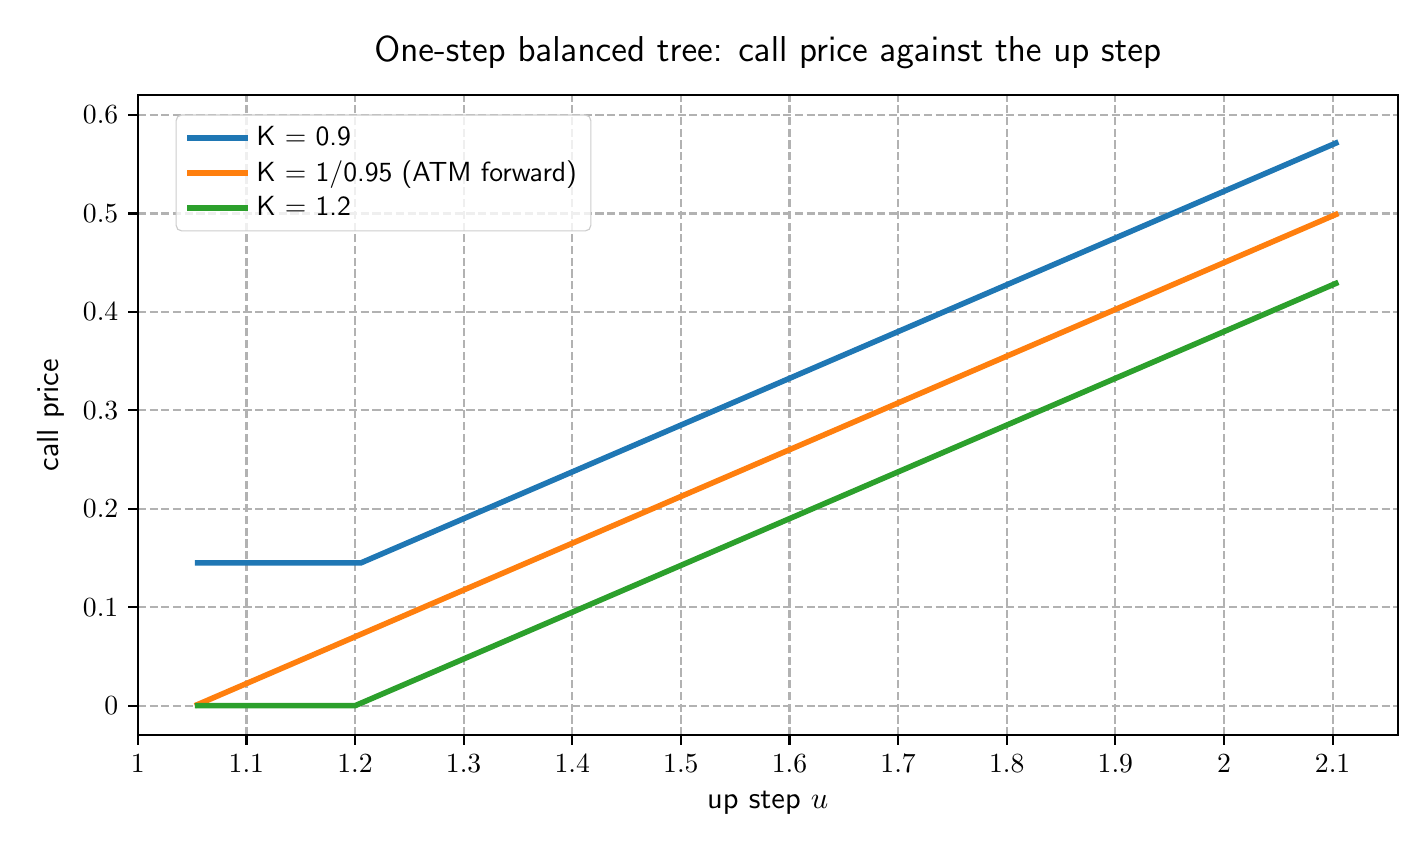
\begin{tikzpicture}
\begin{axis}[mpl, mplgrid, width=6.3in, height=3.2in, xmin=1.0, xmax=2.16, ymin=-0.03, ymax=0.62,
  title={\fontsize{13}{15}\selectfont\sffamily One-step balanced tree: call price against the up step},
  xlabel={\fontsize{11}{13}\selectfont\sffamily up step $u$}, ylabel={\fontsize{11}{13}\selectfont\sffamily call price},
  legend pos=north west, legend style={font=\fontsize{10}{12}\selectfont\sffamily}]
\addplot[tabblue, line width=2pt] coordinates {(1.0526,0.1450) (1.2053,0.1450) (2.1053,0.5725)};
\addlegendentry{K = 0.9}
\addplot[taborange, line width=2pt] coordinates {(1.0526,0.0000) (2.1053,0.5000)};
\addlegendentry{K = 1/0.95 (ATM forward)}
\addplot[tabgreen, line width=2pt] coordinates {(1.0526,0.0000) (1.2000,0.0000) (2.1053,0.4300)};
\addlegendentry{K = 1.2}
\end{axis}
\end{tikzpicture}}
\caption{Output of the one-step check ($S_0=1$, $T=1$, $DF=0.95$). Each price is flat up to $u^*$ and then increases linearly; for the at-the-money-forward strike $u^*=1/DF$, so it increases on the whole range.}
\label{fig:one}
\end{figure}

% ============================================================================ C2, C3 N steps
\subhead{(C2) and (C3) for several steps, and the comparison with Black--Scholes.}
For $N=1,2,5,50$ steps we price the call $S_0=K=1$, $T=1$ with the flat rate of Definition~3 (one-year discount factor $0.95$), for tree volatilities from $0.005$ to $0.6$. Next to it, the Black--Scholes price of Homework~1 with the same rate, $r=-\ln0.95$, and $\sigma=\sigma_{\text{tree}}$:
\par\smallskip\noindent\begin{minipage}{\linewidth}\begin{lstlisting}[style=pysmall,title={check of (C2) and (C3), several steps}]
# (C2), (C3) N-step trees against the tree volatility, and the Black-Scholes price of Homework 1
spot, strike, maturity, df_annual = 1.0, 1.0, 1.0, 0.95
r = -np.log(df_annual)                                   # the same flat interest rate
sigma_grid = np.linspace(0.005, 0.6, 120)
curves, names = [], []
for steps in [1, 2, 5, 50]:
    curves.append([balanced_tree_call_price(spot, strike, maturity, steps, df_annual,
                                            up_step_from_tree_vol(s, maturity, steps, df_annual))
                   for s in sigma_grid])
    names.append(f"tree, N = {steps}")
curves.append([black_scholes_eur_call(r=r, T=maturity, S0=spot, sigma=s, K=strike)[0]
               for s in sigma_grid])         # one sigma at a time (assert sigma > 0)
names.append("Black-Scholes (Homework 1)")

for s in [0.1, 0.2, 0.3]:
    i = np.argmin(np.abs(sigma_grid - s))
    print(f"sigma = {sigma_grid[i]:.3f}: " + "  ".join(f"{c[i]:.4f}" for c in curves))
print("increasing:", [bool(np.all(np.diff(c) >= -1e-12)) for c in curves])

fig, ax = my_plotter(sigma_grid, curves,
                     layout={"title": "Call price against the tree volatility (S0 = K = 1, T = 1)",
                             "x_label": "tree volatility $(u - 1/DF)/\\sqrt{\\Delta t}$, or $\\sigma$",
                             "y_label": "call price", "hline": None, "grid": True, "figsize": (8, 4),
                             "title_fontsize": 13, "label_fontsize": 11, "legend_fontsize": 10,
                             "linewidth": 2, "linestyles": ["-", "-", "-", "-", "--"],
                             "colors": ["tab:blue", "tab:orange", "tab:green", "tab:red", "black"]},
                     names=names)
\end{lstlisting}
\begin{lstlisting}[style=out,title={output (columns: N = 1, 2, 5, 50, Black-Scholes)}]
sigma = 0.100: 0.0725  0.0708  0.0671  0.0690  0.0689
sigma = 0.200: 0.1200  0.1017  0.1076  0.1055  0.1052
sigma = 0.300: 0.1675  0.1302  0.1480  0.1426  0.1429
increasing: [True, True, True, True, True]
\end{lstlisting}\end{minipage}\par\smallskip
All five curves of Figure~\ref{fig:multi} are increasing (the line \texttt{increasing}), and the tree with $50$ steps is already close to the Black--Scholes price: $0.0690$ against $0.0689$ at $\sigma=0.1$, $0.1055$ against $0.1052$ at $\sigma=0.2$. The Black--Scholes price is strictly increasing in $\sigma$ by Theorem~1, \eqref{eq:vega}; the tree prices behave in the same way in the step size, which is the meaning of (C1)--(C3).

\begin{figure}[!ht]
\centering
\resizebox{0.72\textwidth}{!}{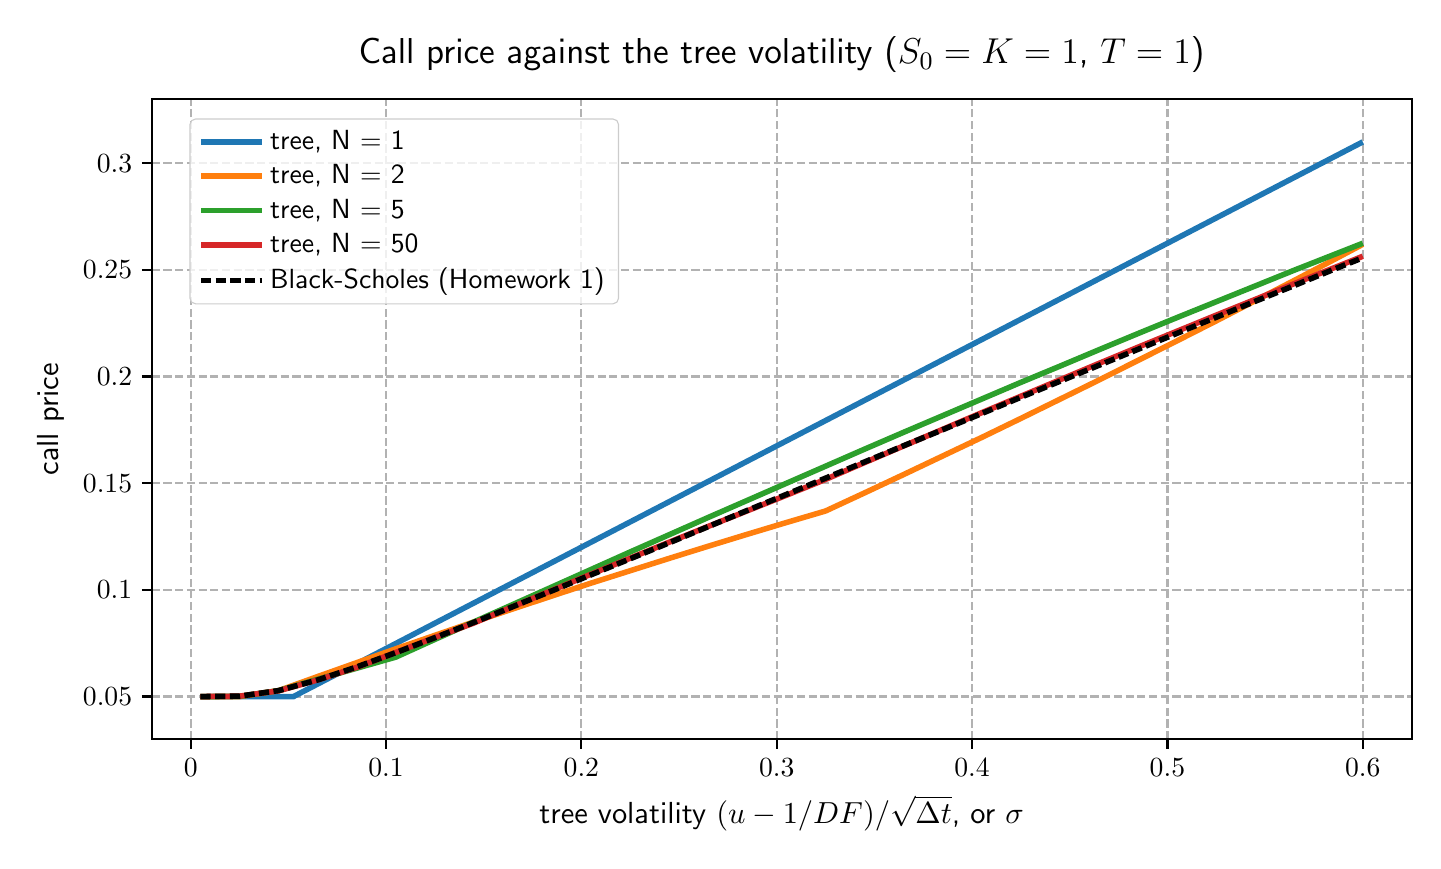
\begin{tikzpicture}
\begin{axis}[mpl, mplgrid, width=6.3in, height=3.2in, xmin=-0.02, xmax=0.625, ymin=0.03, ymax=0.33,
  xtick={0,0.1,0.2,0.3,0.4,0.5,0.6}, ytick={0.05,0.1,0.15,0.2,0.25,0.3},
  xticklabel style={/pgf/number format/fixed}, yticklabel style={/pgf/number format/fixed, /pgf/number format/precision=2},
  title={\fontsize{13}{15}\selectfont\sffamily Call price against the tree volatility ($S_0 = K = 1$, $T = 1$)},
  xlabel={\fontsize{11}{13}\selectfont\sffamily tree volatility $(u - 1/DF)/\sqrt{\Delta t}$, or $\sigma$}, ylabel={\fontsize{11}{13}\selectfont\sffamily call price},
  legend pos=north west, legend style={font=\fontsize{10}{12}\selectfont\sffamily}]
\addplot[tabblue, line width=2pt] coordinates {(0.0050,0.0500) (0.0526,0.0500) (0.6000,0.3100)};
\addlegendentry{tree, N = 1}
\addplot[taborange, line width=2pt] coordinates {(0.0050,0.0500) (0.0250,0.0500) (0.0450,0.0528) (0.0650,0.0594) (0.0850,0.0659) (0.1050,0.0724) (0.1250,0.0787) (0.1450,0.0850) (0.1650,0.0911) (0.1850,0.0972) (0.2050,0.1032) (0.2250,0.1090) (0.2450,0.1148) (0.2650,0.1205) (0.2850,0.1261) (0.3050,0.1316) (0.3250,0.1370) (0.3450,0.1455) (0.3650,0.1541) (0.3850,0.1628) (0.4050,0.1715) (0.4250,0.1804) (0.4450,0.1894) (0.4650,0.1984) (0.4850,0.2076) (0.5050,0.2168) (0.5250,0.2261) (0.5450,0.2356) (0.5650,0.2451) (0.5850,0.2547) (0.6000,0.2620)};
\addlegendentry{tree, N = 2}
\addplot[tabgreen, line width=2pt] coordinates {(0.0050,0.0500) (0.0250,0.0501) (0.0450,0.0528) (0.0650,0.0581) (0.0850,0.0633) (0.1050,0.0685) (0.1250,0.0768) (0.1450,0.0850) (0.1650,0.0932) (0.1850,0.1014) (0.2050,0.1096) (0.2250,0.1178) (0.2450,0.1259) (0.2650,0.1340) (0.2850,0.1420) (0.3050,0.1500) (0.3250,0.1580) (0.3450,0.1660) (0.3650,0.1739) (0.3850,0.1817) (0.4050,0.1895) (0.4250,0.1973) (0.4450,0.2049) (0.4650,0.2126) (0.4850,0.2202) (0.5050,0.2277) (0.5250,0.2351) (0.5450,0.2425) (0.5650,0.2499) (0.5850,0.2571) (0.6000,0.2625)};
\addlegendentry{tree, N = 5}
\addplot[tabred, line width=2pt] coordinates {(0.0050,0.0500) (0.0250,0.0502) (0.0450,0.0527) (0.0650,0.0578) (0.0850,0.0637) (0.1050,0.0707) (0.1250,0.0777) (0.1450,0.0845) (0.1650,0.0922) (0.1850,0.0998) (0.2050,0.1074) (0.2250,0.1149) (0.2450,0.1224) (0.2650,0.1298) (0.2850,0.1371) (0.3050,0.1444) (0.3250,0.1518) (0.3450,0.1597) (0.3650,0.1675) (0.3850,0.1753) (0.4050,0.1831) (0.4250,0.1908) (0.4450,0.1985) (0.4650,0.2062) (0.4850,0.2138) (0.5050,0.2213) (0.5250,0.2288) (0.5450,0.2362) (0.5650,0.2436) (0.5850,0.2509) (0.6000,0.2564)};
\addlegendentry{tree, N = 50}
\addplot[black, line width=2pt, mpldash] coordinates {(0.0050,0.0500) (0.0250,0.0502) (0.0450,0.0528) (0.0650,0.0578) (0.0850,0.0639) (0.1050,0.0706) (0.1250,0.0776) (0.1450,0.0848) (0.1650,0.0922) (0.1850,0.0996) (0.2050,0.1071) (0.2250,0.1146) (0.2450,0.1221) (0.2650,0.1297) (0.2850,0.1373) (0.3050,0.1448) (0.3250,0.1524) (0.3450,0.1600) (0.3650,0.1676) (0.3850,0.1751) (0.4050,0.1827) (0.4250,0.1903) (0.4450,0.1978) (0.4650,0.2053) (0.4850,0.2128) (0.5050,0.2203) (0.5250,0.2278) (0.5450,0.2353) (0.5650,0.2427) (0.5850,0.2502) (0.6000,0.2557)};
\addlegendentry{Black-Scholes (Homework 1)}
\end{axis}
\end{tikzpicture}}
\caption{Output of the check with several steps. The tree prices increase with the step size like the Black--Scholes price increases with $\sigma$, and approach it as $N$ grows.}
\label{fig:multi}
\end{figure}

\ansbox{Hence the background holds, with the step size $h=u-1/DF$ in the role of the volatility:
\begin{itemize}
\item \textbf{(C1)} in a balanced tree $d=2/DF-u$ (Lemma~1); one step has mean $1/DF$, fixed by the interest rate, and standard deviation $u-1/DF$ (Lemma~2), like $\sigma\sqrt{\Delta t}$ in Black--Scholes;
\item \textbf{(C2)} the call price does not decrease when the up step increases (Lemma~3 for one step, Figures~\ref{fig:one} and~\ref{fig:multi}), as the Black--Scholes price increases with $\sigma$ (Theorem~1);
\item \textbf{(C3)} once the strike lies between the leaves, the price is strictly increasing and continuous in $u$, so each attainable price comes from exactly one up step; for one step, \eqref{eq:range}: $u\in[u^*,2/DF)$ and $V_0\in[(S_0-DF\,K)^+,\ S_0-DF\,K/2)$.
\end{itemize}}

\noindent\emph{Comment (to keep in mind for the Task).} The 1--1 correspondence needs two conditions. First, the price is flat for small steps, as long as all leaves are on the same side of the strike (for one step, $u\le u^*$); there the price is the lower bound $(S_0-DF^N K)^+$, and every $u$ in the flat part gives it. Second, not every price can be reached: $d>0$ bounds the up step by $2/DF$, so for one step the price stays below $S_0-DF\,K/2$. So the calibration of part 2 must check that the given price lies in the attainable range and must look for $u$ above the flat part; with more steps the flat part is very short (Figure~\ref{fig:multi}).


\newpage
\parthead{Part 2: Task}\label{part2}

\noindent\textbf{Remark.} The results used are those of Part~1, cited by number; no new result is needed: everything comes from the lecture, Homework~1 and Lemmas~1--2 of Part~1 (sources in the References at the end). The code shown is an exact copy of the files, can be copied from this PDF into Python, and every number is printed by it (files \texttt{*.out}; the extra columns of Tables~\ref{tab:A} and~\ref{tab:Bp} in \texttt{outputs.txt}, printed by \texttt{run\_all.py}). Files: \texttt{calibrator.py} (new), \texttt{bg\_functions.py} (part 1, one short change), \texttt{prof\_tree.py} (lecture), \texttt{hw1\_call.py}, \texttt{plotter.py} (Homework~1), the runs \texttt{q1\_calibrate\_test.py}, \texttt{demo\_A.py}, \texttt{demo\_B.py}, the pictures \texttt{tree\_plot.py}, \texttt{trees\_demo.py}, and the notebooks \texttt{2\_HW\_EXE\_2} (Q1), \texttt{2\_HW\_EXE\_3} (Q2), \texttt{2\_HW\_EXE\_4} (Q3), \texttt{2\_HW\_EXE\_5} (Q4 trees) with the same code.

% ============================================================================ assignment + plan
\subhead{The assignment.}
\emph{Task: Write a calibrate method which, for a given number of steps parameter, computes the up step size for which a Balanced Binomial Tree model returns the specified price for a given European call. (In practice option prices can be observed in the market, so it makes sense to assume it is given). Demonstrate the calibrate method for various input parameters (same contract with a few different number of steps (dont forget to scale the discount factor to keep interest rates flat); calibrate one step tree for various contracts (different expiries and strike levels, flat interest rate)). Make simple plots to illustrate results.}

\noindent\emph{Hint: To do it you will need to use a root solver, I recommend using scipy.optimize.minimize.}

\subhead{What will be done (plan).}
Notation: $V(u)$ is the call price of the balanced tree with up step $u$, all other parameters fixed (\texttt{balanced\_tree\_call\_price} of part 1). The given (``market'') price $V^*$ is the Black--Scholes price of Homework~1 with $\sigma=0.2$ and the flat rate of the tree, $r=-\ln0.95$. Running example: $S_0=K=1$, $T=1$, $DF_1=0.95$, $V^*=0.105195$.
\begin{itemize}
\item \textbf{Q1.} Write \texttt{calibrate}: from $V^*,S_0,K,T,N,DF_1$ return the $u$ with $V(u)=V^*$, in five steps (Figure~\ref{fig:cal}); test it.
\item \textbf{Q2 (Demo A).} Same contract, $N=1,2,3,5,10,20,50,100$ steps, discount factor scaled (Definition~3).
\item \textbf{Q3 (Demo B).} One-step tree, $T\in\{0.25,0.5,1,2\}$, $K\in\{0.8,0.9,1.0,1.1,1.2\}$, flat rate.
\item \textbf{Q4 (plots).} Inside Q1--Q3: $V(u)$ against $u$; $u$ and tree volatility against $N$ and against $K$; and pictures of the calibrated trees (spot tree and price tree of the lecture code) for $N=2,5,50$.
\end{itemize}

\begin{center}
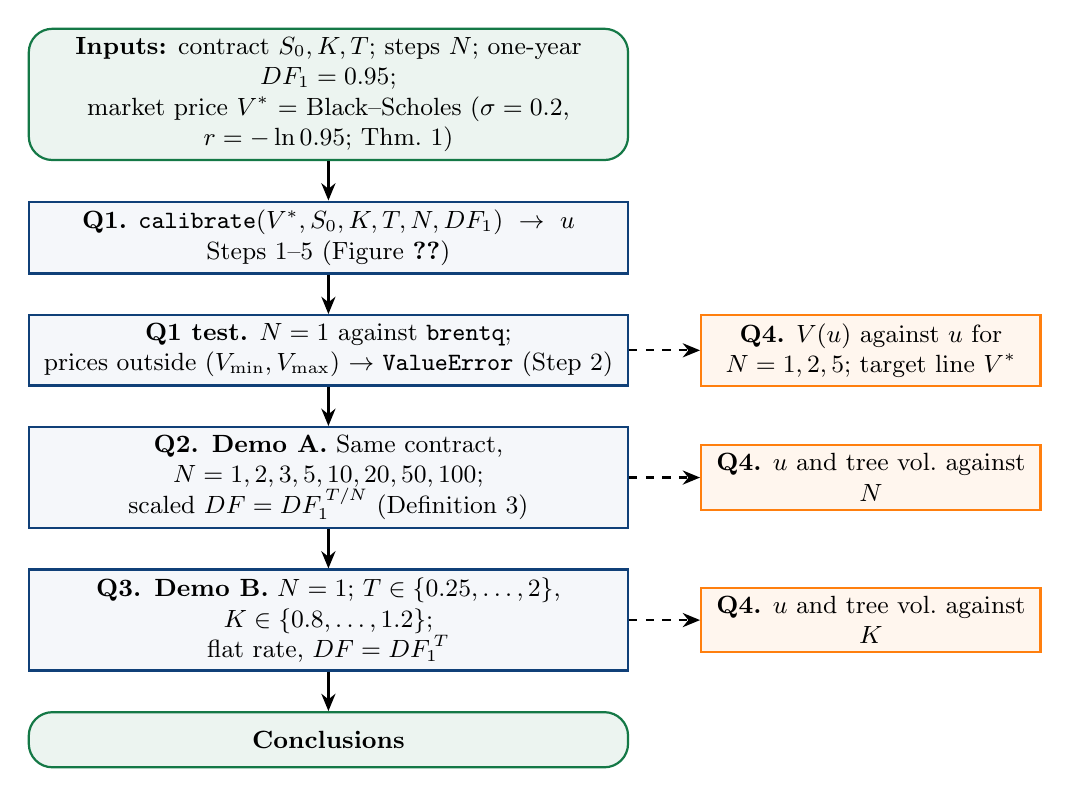
\begin{tikzpicture}[node distance=5mm and 9mm]
\node[fcterm, text width=7.4cm] (in) {\textbf{Inputs:} contract $S_0,K,T$; steps $N$; one-year $DF_1=0.95$;\\ market price $V^*$ = Black--Scholes ($\sigma=0.2$, $r=-\ln0.95$; Thm.~1)};
\node[fcbox, text width=7.4cm, below=of in] (q1) {\textbf{Q1.} \texttt{calibrate}$(V^*,S_0,K,T,N,DF_1)\ \to\ u$\\ Steps 1--5 (Figure~\ref{fig:cal})};
\node[fcbox, text width=7.4cm, below=of q1] (t1) {\textbf{Q1 test.} $N=1$ against \texttt{brentq};\\ prices outside $(V_{\min},V_{\max})$ $\to$ \texttt{ValueError} (Step 2)};
\node[fcbox, text width=7.4cm, below=of t1] (qa) {\textbf{Q2. Demo A.} Same contract, $N=1,2,3,5,10,20,50,100$;\\ scaled $DF=DF_1^{\,T/N}$ (Definition~3)};
\node[fcbox, text width=7.4cm, below=of qa] (qb) {\textbf{Q3. Demo B.} $N=1$; $T\in\{0.25,\dots,2\}$, $K\in\{0.8,\dots,1.2\}$;\\ flat rate, $DF=DF_1^{\,T}$};
\node[fcterm, text width=7.4cm, below=of qb] (end) {\textbf{Conclusions}};
\node[fcplot, text width=4.1cm, right=of t1] (p1) {\textbf{Q4.} $V(u)$ against $u$ for $N=1,2,5$; target line $V^*$};
\node[fcplot, text width=4.1cm, right=of qa] (p2) {\textbf{Q4.} $u$ and tree vol.\ against $N$};
\node[fcplot, text width=4.1cm, right=of qb] (p3) {\textbf{Q4.} $u$ and tree vol.\ against $K$};
\foreach \a/\b in {in/q1, q1/t1, t1/qa, qa/qb, qb/end} \draw[fcarr] (\a) -- (\b);
\foreach \a/\b in {t1/p1, qa/p2, qb/p3} \draw[fcarr, dashed] (\a) -- (\b);
\end{tikzpicture}
\captionof{figure}{Master flowchart: what is done in this part.}\label{fig:plan}
\end{center}

% ============================================================================ results

\subhead{Results used.}
The results of Part~1, cited by number: Definition~1 (risk-neutral price, \eqref{eq:VN}), Definition~2 (balanced tree, \eqref{eq:bal}), Definition~3 (flat rate, $DF=DF_1^{\,T/N}$, \eqref{eq:flat}), Theorem~1 (vega of the Black--Scholes call, \eqref{eq:vega}), Lemma~1 (balanced down step $d=2/DF-u$, \eqref{eq:down}, with $u\in(\frac1{DF},\frac2{DF})$) and Lemma~2 (one step has mean $\frac1{DF}$ and standard deviation $h=u-\frac1{DF}$). Theorem~1 is used only to fix the market price: $V^*=c$ with $\sigma=0.2$ and $r=-\ln DF_1$, a price that ``contains'' the volatility $0.2$. From Lemma~2, as in (C1) of Part~1, the \emph{tree volatility} is
\begin{equation}\label{eq:vol}
\sigma_{\text{tree}}=\frac{u-1/DF}{\sqrt{\Delta t}}
\end{equation}
(\texttt{tree\_vol} below; it is the inverse of \texttt{up\_step\_from\_tree\_vol} of Part~1).

\noindent\emph{Sources of Lemmas 1--2.} \emph{Lemma~1:} put $\tilde p=\frac12$ (Definition~2) in $\tilde p$ of Definition~1, with $1+r=1/DF$, and solve for $d$ (proof in Part~1); this is the professor's \texttt{calcBalancedDownStep}, $u-2(u-1/DF)$ (\texttt{Binomial\_tree\_coding.ipynb}, cell 13). The interval comes from the no-arbitrage condition $d<1+r<u$ of the lecture (\texttt{Tree.ipynb}, cell 17) and $d>0$. Book: Shreve~[3], Chapter~1. \emph{Lemma~2:} the mean is $\frac12(u+d)=\frac1{DF}$ by Lemma~1 and both outcomes differ from it by $\pm(u-\frac1{DF})$; a mean growth of $1+r=1/DF$ is the risk-neutral property of the lecture (\texttt{Tree.ipynb}, cell 36; Shreve~[3], Chapter~1). The division by $\sqrt{\Delta t}$ follows the professor's up step in \texttt{Binomial\_tree\_coding.ipynb}, cell 20, $u=\exp\bigl((r-\sigma^2/2)\Delta t+\sigma\sqrt{\Delta t}\bigr)$: ``step sizes are scaled as well''.

\begin{stmbox}{assignment, Background; \texttt{Tree.ipynb}, cell 57}
\emph{``higher step is like higher volatility, it results in higher option prices. Also, there is a 1-1 correspondence between step size and price if all other parameters are fixed.''}\\
In Part~1 this is (C2): $V(u)$ does not decrease when $u$ grows; and (C3): above the flat part $V(u)$ is strictly increasing, so price and $u$ determine each other. Checked in Part~1 by figures for $N=1,2,5,50$.
\end{stmbox}

\subhead{The lecture code used (\texttt{Binomial\_tree\_coding.ipynb}).}
The calibrator prices every tree with the professor's functions, unchanged (file \texttt{prof\_tree.py}; the code is printed in Part~1):
\begin{center}\small
\begin{tabular}{@{}lll@{}}
\toprule
Cell & Function & Role in part 2\\
\midrule
1 & imports (\texttt{numpy}, \texttt{scipy.optimize.minimize}) & \texttt{minimize} is the solver of Step 4 (hint)\\
3 & \texttt{european\_call\_payoff} & call payoff at the leaves\\
5 & \texttt{create\_spot\_tree} & spot tree for $u$ and $d$\\
8 & \texttt{create\_discounted\_price\_tree} & price $V(u)$ = root of the price tree (Def.~1)\\
13 & \texttt{calcBalancedDownStep} & $d=2/DF-u$ (Def.~2, Lemma~1)\\
20 & (scaled discount factor) & $DF=DF_1^{\,T/N}$ (Def.~3; Step 1, Demo A)\\
\bottomrule
\end{tabular}
\end{center}
\begin{center}
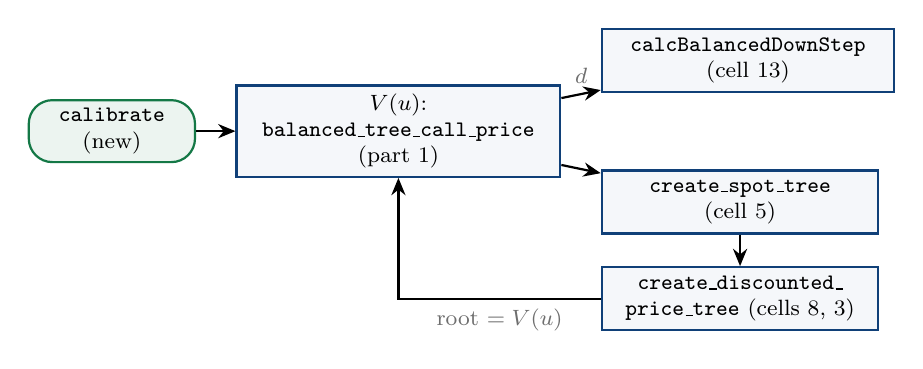
\begin{tikzpicture}[node distance=4mm and 5mm]
\node[fcterm, text width=1.9cm, font=\footnotesize] (c) {\texttt{calibrate}\\(new)};
\node[fcbox, text width=3.9cm, font=\footnotesize, right=of c] (v) {$V(u)$:\\ \texttt{balanced\_tree\_call\_price}\\ (part 1)};
\node[fcbox, text width=3.5cm, font=\footnotesize, right=of v, yshift=9mm] (d) {\texttt{calcBalancedDownStep}\\ (cell 13)};
\node[fcbox, text width=3.3cm, font=\footnotesize, right=of v, yshift=-9mm] (t) {\texttt{create\_spot\_tree}\\ (cell 5)};
\node[fcbox, text width=3.3cm, font=\footnotesize, below=of t] (pt) {\texttt{create\_discounted\_}\\\texttt{price\_tree} (cells 8, 3)};
\draw[fcarr] (c) -- (v);
\draw[fcarr] (v) -- node[above, fclab] {$d$} (d);
\draw[fcarr] (v) -- (t);
\draw[fcarr] (t) -- (pt);
\draw[fcarr] (pt.west) -| node[pos=0.25, below, fclab] {root $=V(u)$} (v.south);
\end{tikzpicture}
\end{center}
\noindent Test of the lecture code (cells 6 and 14; first cells of \texttt{2\_HW\_EXE\_2}): balanced 2-step tree, $u=1.2$, $DF=0.95$, $K=1$ gives the lecture's price tree \texttt{[['0.138'], ['0.039', '0.237'], ['0.000', '0.078', '0.397']]}. Not used: the barrier cells 17--21.

\noindent Which prices can be calibrated is decided numerically in Step~2 (tree prices at the two ends of the interval of $u$), with the statement of the professor; no new result is needed.

% ============================================================================ Q1
\subhead{Q1 --- the \texttt{calibrate} method.}
\textbf{Idea.} By the statement of the professor ((C2), (C3) of Part~1), $V(u)$ does not decrease on $(1/DF,2/DF)$; near $1/DF$ it can be constant (the flat part of Figure~\ref{fig:q1}), above it is strictly increasing. So \texttt{calibrate} checks that $V^*$ is attainable, brackets the solution above the flat part, minimizes the squared error there (the hint) and checks the result:

\begin{center}
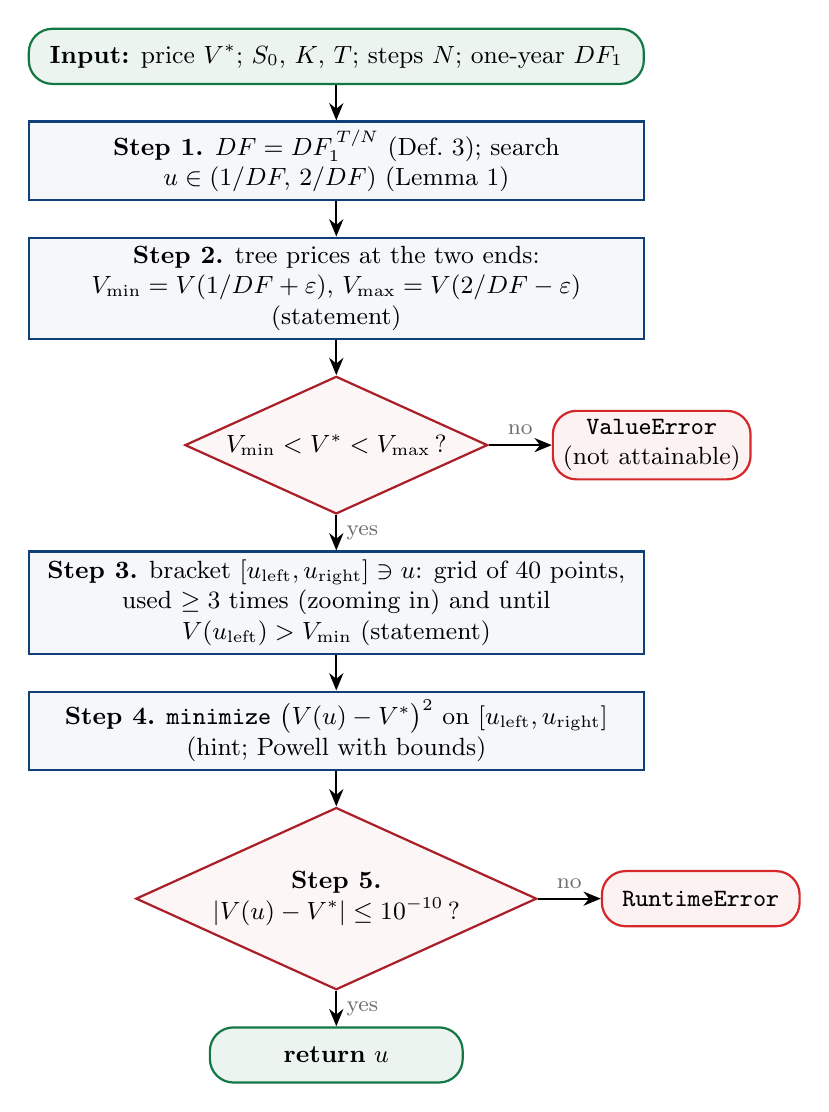
\begin{tikzpicture}[node distance=4.5mm and 8mm]
\node[fcterm, text width=7.6cm] (in) {\textbf{Input:} price $V^*$; $S_0$, $K$, $T$; steps $N$; one-year $DF_1$};
\node[fcbox, text width=7.6cm, below=of in] (s1) {\textbf{Step 1.} $DF=DF_1^{\,T/N}$ (Def.~3); search $u\in(1/DF,\,2/DF)$ (Lemma~1)};
\node[fcbox, text width=7.6cm, below=of s1] (s2) {\textbf{Step 2.} tree prices at the two ends: $V_{\min}=V(1/DF+\varepsilon)$, $V_{\max}=V(2/DF-\varepsilon)$ (statement)};
\node[fcdec, below=of s2] (d2) {$V_{\min}<V^*<V_{\max}$\,?};
\node[fcerr, text width=2.3cm, right=of d2] (e2) {\texttt{ValueError}\\(not attainable)};
\node[fcbox, text width=7.6cm, below=of d2] (s3) {\textbf{Step 3.} bracket $[\ul,\ur]\ni u$: grid of 40 points, used $\ge3$ times (zooming in) and until $V(\ul)>V_{\min}$ (statement)};
\node[fcbox, text width=7.6cm, below=of s3] (s4) {\textbf{Step 4.} \texttt{minimize} $\bigl(V(u)-V^*\bigr)^2$ on $[\ul,\ur]$ (hint; Powell with bounds)};
\node[fcdec, below=of s4] (d5) {\textbf{Step 5.}\\ $|V(u)-V^*|\le10^{-10}$\,?};
\node[fcerr, text width=2.3cm, right=of d5] (e5) {\texttt{RuntimeError}};
\node[fcterm, text width=3cm, below=of d5] (out) {\textbf{return} $u$};
\foreach \a/\b in {in/s1, s1/s2, s2/d2, s3/s4, s4/d5} \draw[fcarr] (\a) -- (\b);
\draw[fcarr] (d2) -- node[right, fclab] {yes} (s3);
\draw[fcarr] (d2) -- node[above, fclab] {no} (e2);
\draw[fcarr] (d5) -- node[right, fclab] {yes} (out);
\draw[fcarr] (d5) -- node[above, fclab] {no} (e5);
\end{tikzpicture}
\captionof{figure}{Flowchart of \texttt{calibrate} (file \texttt{calibrator.py}).}\label{fig:cal}
\end{center}

\step{Step 1 (one-step $DF$ and the interval of $u$).} \texttt{df\_annual ** (maturity / steps)} is $DF=DF_1^{\,T/N}$, which keeps the rate flat (Definition~3, \eqref{eq:flat}). A balanced tree needs $1/DF<u<2/DF$ (Lemma~1, \eqref{eq:down}): these are \texttt{u\_low}, \texttt{u\_high}.

\step{Step 2 (is $V^*$ attainable?).} The function \texttt{price\_range} prices the tree at the two ends of the interval: $V_{\min}=V(1/DF+\varepsilon)$, $V_{\max}=V(2/DF-\varepsilon)$, $\varepsilon=10^{-10}/DF$. Since $V$ does not decrease (statement), every $u$ gives a price in $[V_{\min},V_{\max}]$; if $V^*\notin(V_{\min},V_{\max})$, \texttt{calibrate} raises \texttt{ValueError}.

\begin{center}
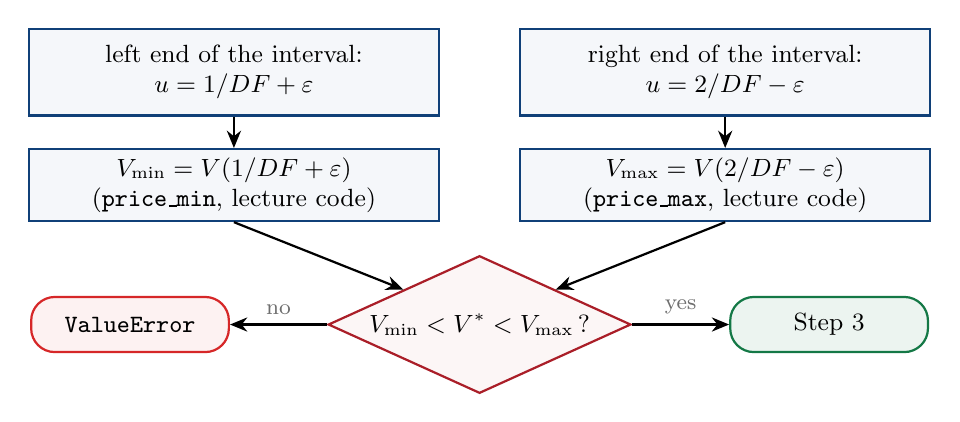
\begin{tikzpicture}[node distance=4mm and 10mm]
\node[fcbox, text width=5cm, minimum height=11mm] (l1) {left end of the interval:\\ $u=1/DF+\varepsilon$};
\node[fcbox, text width=5cm, minimum height=11mm, right=of l1] (l2) {right end of the interval:\\ $u=2/DF-\varepsilon$};
\node[fcbox, text width=5cm, below=of l1] (v1) {$V_{\min}=V(1/DF+\varepsilon)$\\ (\texttt{price\_min}, lecture code)};
\node[fcbox, text width=5cm, below=of l2] (v2) {$V_{\max}=V(2/DF-\varepsilon)$\\ (\texttt{price\_max}, lecture code)};
\node[fcdec] (d) at ($(v1.south)!0.5!(v2.south)+(0,-1.3)$) {$V_{\min}<V^*<V_{\max}$\,?};
\node[fcerr, text width=2.3cm] (e) at ($(v1.south west)+(1.3,-1.3)$) {\texttt{ValueError}};
\node[fcterm, text width=2.3cm] (go) at ($(v2.south east)+(-1.3,-1.3)$) {Step 3};
\draw[fcarr] (l1) -- (v1); \draw[fcarr] (l2) -- (v2);
\draw[fcarr] (v1.south) -- (d.north west);
\draw[fcarr] (v2.south) -- (d.north east);
\draw[fcarr] (d) -- node[above, fclab] {no} (e);
\draw[fcarr] (d) -- node[above, fclab] {yes} (go);
\end{tikzpicture}
\captionof{figure}{Step 2: the tree prices at the two ends of the interval and the test.}\label{fig:s2}
\end{center}

\step{Step 3 (bracket).} On a grid of $40$ points of $(u_{\text{low}},u_{\text{high}})$ (moved inside by $\varepsilon=10^{-10}u_{\text{low}}$), take the first point $u_k$ with $V(u_k)\ge V^*$. Since $V$ does not decrease (statement), the solution lies in $[u_{k-1},u_k]$.
\begin{itemize}
\item Zoom: the same grid on $[u_{k-1},u_k]$ ($39$ times shorter). Grids: at least $3$ (\texttt{n\_zoom}: whole interval, then $2$ zooms; at most $30$) and until $V(\ul)>V_{\min}$ (code: $V_{\min}+10^{-12}$). Then the bracket is above the flat part, where $V$ is strictly increasing: unique solution (statement).
\end{itemize}

\begin{center}
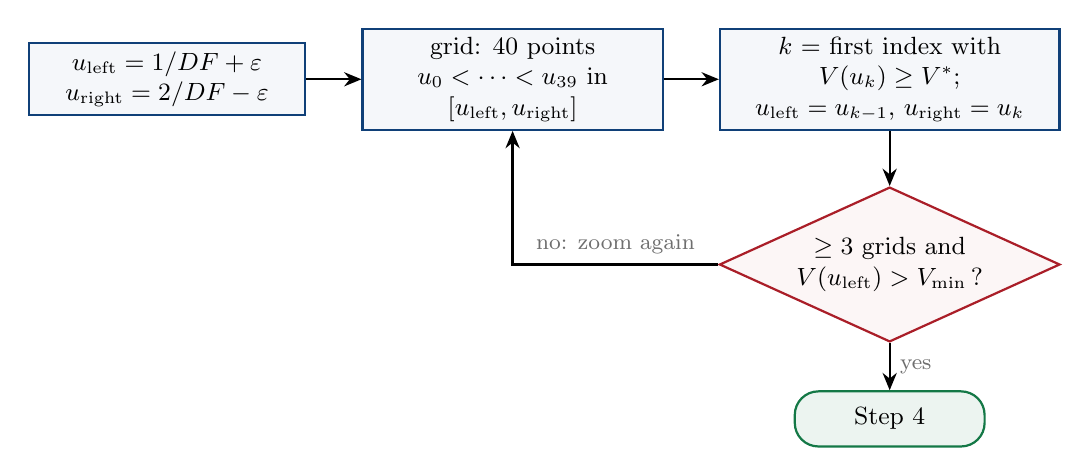
\begin{tikzpicture}[node distance=5mm and 7mm]
\node[fcbox, text width=3.3cm] (a) {$\ul=1/DF+\varepsilon$\\ $\ur=2/DF-\varepsilon$};
\node[fcbox, text width=3.6cm, right=of a] (b) {grid: $40$ points\\ $u_0<\dots<u_{39}$ in $[\ul,\ur]$};
\node[fcbox, text width=4.1cm, right=of b] (c) {$k$ = first index with $V(u_k)\ge V^*$;\\ $\ul=u_{k-1}$, $\ur=u_k$};
\node[fcdec, below=7mm of c] (d) {$\ge3$ grids and\\ $V(\ul)>V_{\min}$\,?};
\node[fcterm, text width=2.2cm, below=6mm of d] (go) {Step 4};
\draw[fcarr] (a) -- (b); \draw[fcarr] (b) -- (c); \draw[fcarr] (c) -- (d);
\draw[fcarr] (d) -- node[right, fclab] {yes} (go);
\draw[fcarr] (d.west) -| node[pos=0.25, above, fclab] {no: zoom again} (b.south);
\end{tikzpicture}
\captionof{figure}{Step 3: bracketing by zooming in.}\label{fig:s3}
\end{center}

\step{Step 4 (minimize).} As the hint says, \texttt{scipy.optimize.minimize} is applied to $f(u)=\bigl(V(u)-V^*\bigr)^2$ on the bracket: $f\ge0$, and $f=0$ only at the calibrated $u$ (unique in the bracket by Step 3). Method \texttt{"Powell"} (no derivatives, accepts bounds), start at the middle of the bracket.

\begin{center}
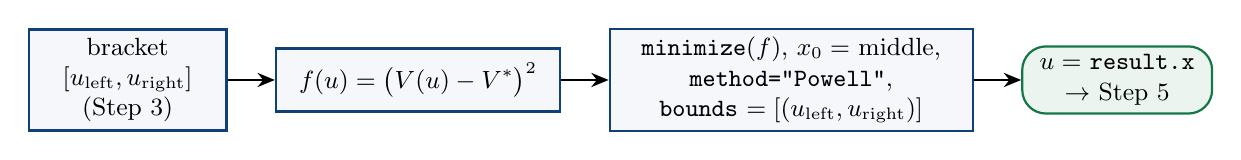
\begin{tikzpicture}[node distance=5mm and 6mm]
\node[fcbox, text width=2.3cm] (a) {bracket $[\ul,\ur]$\\ (Step 3)};
\node[fcbox, text width=3.4cm, right=of a] (b) {$f(u)=\bigl(V(u)-V^*\bigr)^2$};
\node[fcbox, text width=4.4cm, right=of b] (c) {\texttt{minimize}$(f)$, $x_0=$ middle,\\ \texttt{method="Powell"},\\ \texttt{bounds} $=[(\ul,\ur)]$};
\node[fcterm, text width=2.2cm, right=of c] (d) {$u=$ \texttt{result.x}\\ $\to$ Step 5};
\draw[fcarr] (a) -- (b); \draw[fcarr] (b) -- (c); \draw[fcarr] (c) -- (d);
\end{tikzpicture}
\captionof{figure}{Step 4: the minimization of the hint.}\label{fig:s4}
\end{center}

\step{Step 5 (check).} The error $V(u)-V^*$ is computed with the tree again; if $|V(u)-V^*|>10^{-10}$ \texttt{calibrate} raises \texttt{RuntimeError}, otherwise it returns $u$. So the returned $u$ really gives ``the specified price''.

\needspace{0.8\textheight}
\subhead{Q1 --- the code.} The new file (Steps 1--5 are marked in the comments):
\par\smallskip\noindent\begin{minipage}{\linewidth}\begin{lstlisting}[style=pysmall,title={new code (\texttt{calibrator.py})}]
"""Homework 2, part 2 (Task): calibrator for the Balanced Binomial Tree.

calibrate(...) returns the up step u for which the balanced tree (p_up = p_down = 0.5)
prices a given European call at a given price. Steps 1-5 follow the flowchart of the report.
"""
import numpy as np
from scipy.optimize import minimize

from bg_functions import balanced_tree_call_price


def price_range(spot: float, strike: float, maturity: float, steps: int,
                df_annual: float) -> tuple[float, float]:
    """Tree prices at the two ends of the interval of u (Lemma 1): u_low + eps, u_high - eps.
    The price does not decrease in u (statement of the professor), so every u gives a price
    between these two values."""
    discount_factor = df_annual ** (maturity / steps)
    u_low, u_high = 1 / discount_factor, 2 / discount_factor
    eps = 1e-10 * u_low
    price_min = balanced_tree_call_price(spot, strike, maturity, steps, df_annual, u_low + eps)
    price_max = balanced_tree_call_price(spot, strike, maturity, steps, df_annual, u_high - eps)
    return price_min, price_max


def tree_vol(spot_mult_up: float, maturity: float, steps: int, df_annual: float) -> float:
    """Tree volatility (u - 1/DF) / sqrt(dt) of part 1 (inverse of up_step_from_tree_vol)."""
    dt = maturity / steps
    return (spot_mult_up - 1 / df_annual ** dt) / np.sqrt(dt)


def calibrate(price: float, spot: float, strike: float, maturity: float, steps: int,
              df_annual: float, n_grid: int = 40, n_zoom: int = 3,
              tol: float = 1e-10) -> float:
    """Up step u such that balanced_tree_call_price(..., u) = price."""
    # Step 1: discount factor of one step (flat rate, Definition 3) and the interval of u
    discount_factor = df_annual ** (maturity / steps)
    u_low, u_high = 1 / discount_factor, 2 / discount_factor      # d < 1/DF < u and d > 0
    # Step 2: is the price attainable? (tree prices at the two ends of the interval)
    price_min, price_max = price_range(spot, strike, maturity, steps, df_annual)
    if not price_min < price < price_max:
        raise ValueError(f"price {price:.6f} not attainable: it must lie in "
                         f"({price_min:.6f}, {price_max:.6f})")
    # Step 3: bracket the solution. The price is non-decreasing in u (C2), so on a grid of u
    #         the target lies between the last point with price < target and the first point
    #         with price >= target. Zoom in (new grid inside the bracket): use at least n_zoom
    #         grids, and stop when the left end is out of the flat part (price > price_min;
    #         near 1/DF the price can be constant).
    def tree_price(u: float) -> float:
        return balanced_tree_call_price(spot, strike, maturity, steps, df_annual, u)
    eps = 1e-10 * u_low
    u_left, u_right = u_low + eps, u_high - eps
    for zoom in range(30):
        grid = np.linspace(u_left, u_right, n_grid)
        k = next(i for i, u in enumerate(grid) if tree_price(u) >= price)
        u_left, u_right = grid[max(k - 1, 0)], grid[k]
        if zoom + 1 >= n_zoom and tree_price(u_left) > price_min + 1e-12:
            break
    # Step 4: minimize the squared pricing error inside the bracket (hint of the assignment)
    result = minimize(lambda x: (tree_price(x[0]) - price) ** 2, x0=[(u_left + u_right) / 2],
                      method="Powell", bounds=[(u_left, u_right)],
                      options={"xtol": 1e-14, "ftol": 1e-30})
    spot_mult_up = float(np.atleast_1d(result.x)[0])
    # Step 5: check the result
    error = tree_price(spot_mult_up) - price
    if abs(error) > tol:
        raise RuntimeError(f"calibration failed: pricing error {error:.2e}")
    return spot_mult_up
\end{lstlisting}\end{minipage}\par\smallskip
\noindent The part 1 file \texttt{bg\_functions.py} had no imports (they were in the notebook); one change adds them, so that \texttt{calibrator.py} can import it:
\par\smallskip\noindent\begin{minipage}{\linewidth}\begin{lstlisting}[style=py,title={change in \texttt{bg\_functions.py} (top of the file; the rest is the code of part 1)}]
# change # 1  (part 2: imports added so that this file can be imported as a module)
import numpy as np
from prof_tree import create_spot_tree, create_discounted_price_tree, calcBalancedDownStep
# end change # 1
\end{lstlisting}\end{minipage}\par\smallskip

\subhead{Q1 --- test.} (a) $N=1$ against \texttt{scipy.optimize.brentq} (another root solver); (b) two prices outside the range of Step 2; (c) the picture (Q4).
\par\smallskip\noindent\begin{minipage}{\linewidth}\begin{lstlisting}[style=pysmall,title={test (\texttt{q1\_calibrate\_test.py})}]
# Q1: test of calibrate (N = 1 against another root solver, prices out of range, picture)
import numpy as np
from scipy.optimize import brentq
from plotter import my_plotter
from hw1_call import black_scholes_eur_call
from bg_functions import balanced_tree_call_price
from calibrator import calibrate, price_range

spot, strike, maturity, df_annual = 1.0, 1.0, 1.0, 0.95
r = -np.log(df_annual)                                        # the same flat rate
target = black_scholes_eur_call(r=r, T=maturity, S0=spot, sigma=0.2, K=strike)[0]
print(f"target price (Black-Scholes of Homework 1, sigma = 0.2): {target:.6f}")

# (a) one step: calibrate against scipy.optimize.brentq on V(u) - V* (another root solver)
u = calibrate(target, spot, strike, maturity, 1, df_annual)
DF = df_annual ** maturity
u_brentq = brentq(lambda x: balanced_tree_call_price(spot, strike, maturity, 1, df_annual, x)
                  - target, 1 / DF + 1e-10, 2 / DF - 1e-10, xtol=1e-14)
print(f"N = 1: calibrate u = {u:.10f},  brentq u = {u_brentq:.10f}")

# (b) prices that the tree cannot give (Step 2): calibrate raises ValueError
for price in [0.60, 0.04]:
    try:
        calibrate(price, spot, strike, maturity, 1, df_annual)
    except ValueError as error:
        print("ValueError:", error)

# (c) picture: tree price against u for N = 1, 2, 5; the calibrated u is where it meets the target
u_grid = np.linspace(1.0, 1.6, 121)
curves, names, u_cal = [], [], []
for steps in [1, 2, 5]:
    DF = df_annual ** (maturity / steps)
    curves.append([balanced_tree_call_price(spot, strike, maturity, steps, df_annual, x)
                   if 1 / DF < x < 2 / DF else np.nan for x in u_grid])
    u_cal.append(calibrate(target, spot, strike, maturity, steps, df_annual))
    names.append(f"tree, N = {steps}  (u = {u_cal[-1]:.4f})")
fig, ax = my_plotter(u_grid, curves,
                     layout={"title": "Calibration: tree price against the up step u",
                             "x_label": "up step u", "y_label": "call price",
                             "hline": target, "vlines": u_cal, "grid": True,
                             "title_fontsize": 13, "label_fontsize": 11, "legend_fontsize": 10,
                             "linewidth": 2, "colors": ["tab:blue", "tab:orange", "tab:green"],
                             "save_path": "figures/q1_calibration.pdf", "show": False},
                     names=names)
\end{lstlisting}
\begin{lstlisting}[style=out,title={output (\texttt{q1\_calibrate\_test.out})}]
target price (Black-Scholes of Homework 1, sigma = 0.2): 0.105195
N = 1: calibrate u = 1.2214640224,  brentq u = 1.2214640224
ValueError: price 0.600000 not attainable: it must lie in (0.050000, 0.525000)
ValueError: price 0.040000 not attainable: it must lie in (0.050000, 0.525000)
\end{lstlisting}\end{minipage}\par\smallskip

\noindent\textbf{(a)} The two solvers give the same up step:
\begin{align*}
u_{\texttt{calibrate}} &= 1.2214640224\\
&= u_{\texttt{brentq}} && \checkmark
\end{align*}
\textbf{(b)} Step 2 for $N=1$ prints the tree prices at the two ends of the interval, $V_{\min}=0.05$ and $V_{\max}=0.525$ (output); $0.60\ge V_{\max}$ and $0.04\le V_{\min}$, so both raise \texttt{ValueError}.\\
\textbf{(c)} In Figure~\ref{fig:q1} each curve is flat at $V_{\min}=0.05$ near $1/DF$, then increasing, and meets the dashed line $V^*$ exactly once, at the dotted line of its calibrated $u$.

\begin{center}
\resizebox{0.78\textwidth}{!}{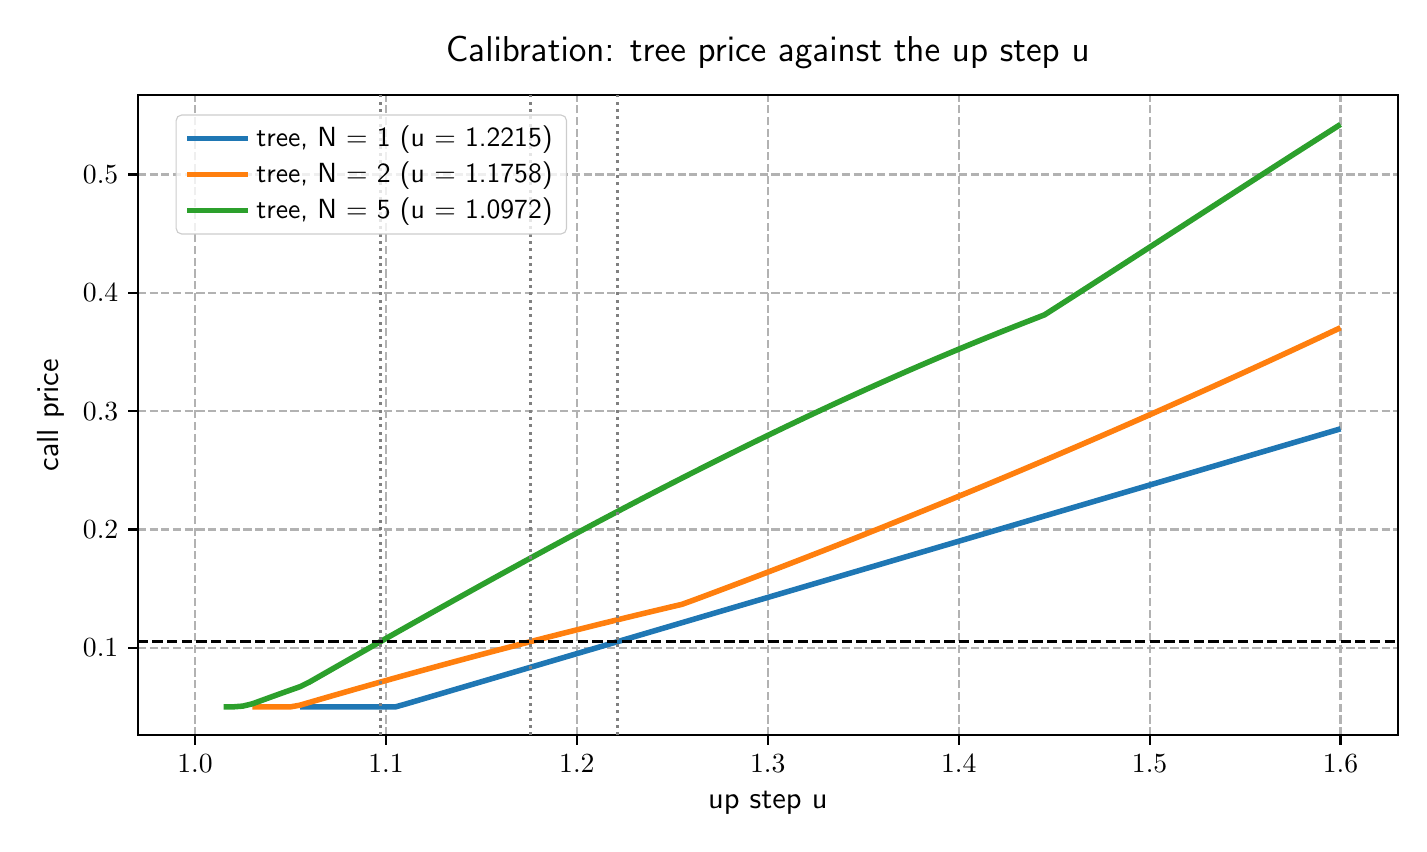
\begin{tikzpicture}
\begin{axis}[mpl, mplgrid, width=6.3in, height=3.2in, xmin=0.97, xmax=1.63, ymin=0.026, ymax=0.567,
  xtick={1.0,1.1,1.2,1.3,1.4,1.5,1.6}, ytick={0.1,0.2,0.3,0.4,0.5},
  xticklabel style={/pgf/number format/fixed, /pgf/number format/precision=1, /pgf/number format/fixed zerofill},
  yticklabel style={/pgf/number format/fixed, /pgf/number format/precision=1},
  title={\fontsize{13}{15}\selectfont\sffamily Calibration: tree price against the up step u},
  xlabel={\fontsize{11}{13}\selectfont\sffamily up step u}, ylabel={\fontsize{11}{13}\selectfont\sffamily call price},
  legend pos=north west, legend style={font=\fontsize{10}{12}\selectfont\sffamily}]
\addplot[tabblue, line width=2pt] coordinates {(1.055,0.05000) (1.060,0.05000) (1.065,0.05000) (1.070,0.05000) (1.075,0.05000) (1.080,0.05000) (1.085,0.05000) (1.090,0.05000) (1.095,0.05000) (1.100,0.05000) (1.105,0.05000) (1.110,0.05225) (1.115,0.05462) (1.120,0.05700) (1.125,0.05937) (1.130,0.06175) (1.135,0.06413) (1.140,0.06650) (1.145,0.06888) (1.150,0.07125) (1.155,0.07363) (1.160,0.07600) (1.165,0.07838) (1.170,0.08075) (1.175,0.08313) (1.180,0.08550) (1.185,0.08788) (1.190,0.09025) (1.195,0.09263) (1.200,0.09500) (1.205,0.09738) (1.210,0.09975) (1.215,0.10213) (1.220,0.10450) (1.225,0.10688) (1.230,0.10925) (1.235,0.11163) (1.240,0.11400) (1.245,0.11638) (1.250,0.11875) (1.255,0.12113) (1.260,0.12350) (1.265,0.12588) (1.270,0.12825) (1.275,0.13063) (1.280,0.13300) (1.285,0.13538) (1.290,0.13775) (1.295,0.14012) (1.300,0.14250) (1.305,0.14488) (1.310,0.14725) (1.315,0.14962) (1.320,0.15200) (1.325,0.15438) (1.330,0.15675) (1.335,0.15912) (1.340,0.16150) (1.345,0.16388) (1.350,0.16625) (1.355,0.16862) (1.360,0.17100) (1.365,0.17338) (1.370,0.17575) (1.375,0.17812) (1.380,0.18050) (1.385,0.18287) (1.390,0.18525) (1.395,0.18762) (1.400,0.19000) (1.405,0.19237) (1.410,0.19475) (1.415,0.19712) (1.420,0.19950) (1.425,0.20187) (1.430,0.20425) (1.435,0.20663) (1.440,0.20900) (1.445,0.21138) (1.450,0.21375) (1.455,0.21613) (1.460,0.21850) (1.465,0.22088) (1.470,0.22325) (1.475,0.22563) (1.480,0.22800) (1.485,0.23038) (1.490,0.23275) (1.495,0.23513) (1.500,0.23750) (1.505,0.23988) (1.510,0.24225) (1.515,0.24463) (1.520,0.24700) (1.525,0.24938) (1.530,0.25175) (1.535,0.25413) (1.540,0.25650) (1.545,0.25888) (1.550,0.26125) (1.555,0.26363) (1.560,0.26600) (1.565,0.26837) (1.570,0.27075) (1.575,0.27313) (1.580,0.27550) (1.585,0.27787) (1.590,0.28025) (1.595,0.28263) (1.600,0.28500)};
\addlegendentry{tree, N = 1  (u = 1.2215)}
\addplot[taborange, line width=2pt] coordinates {(1.030,0.05000) (1.035,0.05000) (1.040,0.05000) (1.045,0.05000) (1.050,0.05000) (1.055,0.05144) (1.060,0.05381) (1.065,0.05616) (1.070,0.05849) (1.075,0.06082) (1.080,0.06313) (1.085,0.06544) (1.090,0.06773) (1.095,0.07001) (1.100,0.07227) (1.105,0.07453) (1.110,0.07677) (1.115,0.07900) (1.120,0.08122) (1.125,0.08343) (1.130,0.08562) (1.135,0.08781) (1.140,0.08998) (1.145,0.09214) (1.150,0.09429) (1.155,0.09642) (1.160,0.09855) (1.165,0.10066) (1.170,0.10276) (1.175,0.10485) (1.180,0.10693) (1.185,0.10899) (1.190,0.11104) (1.195,0.11309) (1.200,0.11512) (1.205,0.11713) (1.210,0.11914) (1.215,0.12113) (1.220,0.12311) (1.225,0.12508) (1.230,0.12704) (1.235,0.12899) (1.240,0.13092) (1.245,0.13284) (1.250,0.13476) (1.255,0.13665) (1.260,0.13956) (1.265,0.14255) (1.270,0.14556) (1.275,0.14859) (1.280,0.15162) (1.285,0.15467) (1.290,0.15772) (1.295,0.16079) (1.300,0.16388) (1.305,0.16697) (1.310,0.17007) (1.315,0.17319) (1.320,0.17632) (1.325,0.17946) (1.330,0.18261) (1.335,0.18578) (1.340,0.18896) (1.345,0.19214) (1.350,0.19534) (1.355,0.19856) (1.360,0.20178) (1.365,0.20502) (1.370,0.20826) (1.375,0.21152) (1.380,0.21480) (1.385,0.21808) (1.390,0.22137) (1.395,0.22468) (1.400,0.22800) (1.405,0.23133) (1.410,0.23467) (1.415,0.23803) (1.420,0.24140) (1.425,0.24477) (1.430,0.24816) (1.435,0.25157) (1.440,0.25498) (1.445,0.25841) (1.450,0.26184) (1.455,0.26529) (1.460,0.26875) (1.465,0.27223) (1.470,0.27571) (1.475,0.27921) (1.480,0.28272) (1.485,0.28624) (1.490,0.28977) (1.495,0.29332) (1.500,0.29687) (1.505,0.30044) (1.510,0.30402) (1.515,0.30762) (1.520,0.31122) (1.525,0.31484) (1.530,0.31846) (1.535,0.32210) (1.540,0.32575) (1.545,0.32942) (1.550,0.33309) (1.555,0.33678) (1.560,0.34048) (1.565,0.34419) (1.570,0.34791) (1.575,0.35165) (1.580,0.35540) (1.585,0.35915) (1.590,0.36292) (1.595,0.36671) (1.600,0.37050)};
\addlegendentry{tree, N = 2  (u = 1.1758)}
\addplot[tabgreen, line width=2pt] coordinates {(1.015,0.05000) (1.020,0.05000) (1.025,0.05064) (1.030,0.05257) (1.035,0.05552) (1.040,0.05845) (1.045,0.06135) (1.050,0.06421) (1.055,0.06705) (1.060,0.07103) (1.065,0.07565) (1.070,0.08026) (1.075,0.08486) (1.080,0.08946) (1.085,0.09405) (1.090,0.09864) (1.095,0.10322) (1.100,0.10779) (1.105,0.11235) (1.110,0.11691) (1.115,0.12145) (1.120,0.12599) (1.125,0.13051) (1.130,0.13503) (1.135,0.13953) (1.140,0.14403) (1.145,0.14851) (1.150,0.15298) (1.155,0.15744) (1.160,0.16188) (1.165,0.16631) (1.170,0.17073) (1.175,0.17513) (1.180,0.17952) (1.185,0.18390) (1.190,0.18826) (1.195,0.19260) (1.200,0.19693) (1.205,0.20124) (1.210,0.20553) (1.215,0.20980) (1.220,0.21406) (1.225,0.21830) (1.230,0.22252) (1.235,0.22672) (1.240,0.23091) (1.245,0.23507) (1.250,0.23921) (1.255,0.24333) (1.260,0.24743) (1.265,0.25151) (1.270,0.25557) (1.275,0.25961) (1.280,0.26362) (1.285,0.26761) (1.290,0.27158) (1.295,0.27552) (1.300,0.27944) (1.305,0.28334) (1.310,0.28721) (1.315,0.29106) (1.320,0.29488) (1.325,0.29867) (1.330,0.30244) (1.335,0.30619) (1.340,0.30990) (1.345,0.31359) (1.350,0.31726) (1.355,0.32089) (1.360,0.32450) (1.365,0.32808) (1.370,0.33164) (1.375,0.33516) (1.380,0.33865) (1.385,0.34212) (1.390,0.34556) (1.395,0.34896) (1.400,0.35234) (1.405,0.35569) (1.410,0.35900) (1.415,0.36229) (1.420,0.36554) (1.425,0.36877) (1.430,0.37196) (1.435,0.37512) (1.440,0.37825) (1.445,0.38143) (1.450,0.38659) (1.455,0.39176) (1.460,0.39693) (1.465,0.40212) (1.470,0.40731) (1.475,0.41250) (1.480,0.41770) (1.485,0.42291) (1.490,0.42812) (1.495,0.43333) (1.500,0.43854) (1.505,0.44376) (1.510,0.44898) (1.515,0.45420) (1.520,0.45942) (1.525,0.46464) (1.530,0.46986) (1.535,0.47507) (1.540,0.48028) (1.545,0.48549) (1.550,0.49070) (1.555,0.49590) (1.560,0.50109) (1.565,0.50628) (1.570,0.51146) (1.575,0.51664) (1.580,0.52180) (1.585,0.52695) (1.590,0.53210) (1.595,0.53723) (1.600,0.54235)};
\addlegendentry{tree, N = 5  (u = 1.0972)}
\addplot[black, line width=1pt, mpldash, forget plot] coordinates {(0.97,0.105195) (1.63,0.105195)};
\addplot[gray, line width=1pt, mpldot, forget plot] coordinates {(1.221464,0.026) (1.221464,0.567)};
\addplot[gray, line width=1pt, mpldot, forget plot] coordinates {(1.175830,0.026) (1.175830,0.567)};
\addplot[gray, line width=1pt, mpldot, forget plot] coordinates {(1.097162,0.026) (1.097162,0.567)};
\end{axis}
\end{tikzpicture}}
\captionof{figure}{Output (c) of the test ($S_0=K=1$, $T=1$, $DF_1=0.95$): tree price $V(u)$ for $N=1,2,5$, the market price $V^*=0.105195$ (dashed) and the calibrated up steps (dotted).}\label{fig:q1}
\end{center}

\ansbox{\textbf{Q1.} \texttt{calibrate(price, spot, strike, maturity, steps, df\_annual)} (file \texttt{calibrator.py}) returns the up step $u$ for which the balanced tree with \texttt{steps} steps returns the given call price, with error at most $10^{-10}$. Running example ($V^*=0.105195$): $u=1.2214640224$ for $N=1$, equal to the \texttt{brentq} solution; $u=1.1758$ for $N=2$ and $u=1.0972$ for $N=5$ (Figure~\ref{fig:q1}). A price outside $(V_{\min},V_{\max})$ of Step 2, here $(0.05,\,0.525)$, raises \texttt{ValueError}.}

% ============================================================================ Q2
\subhead{Q2 --- Demo A: the same contract with several numbers of steps.}
Contract $S_0=K=1$, $T=1$, $V^*=0.105195$; for each $N$ the discount factor is scaled, $DF=0.95^{1/N}$ (Definition~3), so the rate stays flat. After \texttt{calibrate} we compute $d$ (Lemma~1), the error, and the tree volatility (Lemma~2, \eqref{eq:vol}).

\begin{center}
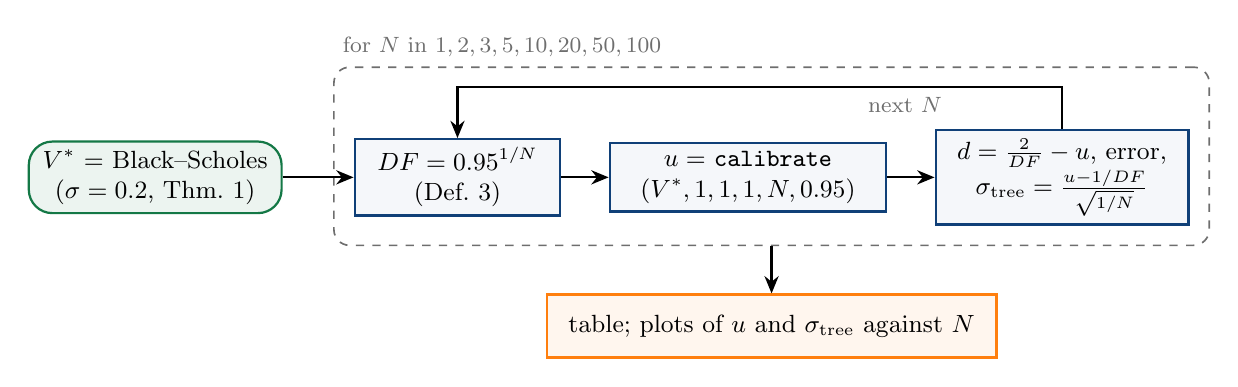
\begin{tikzpicture}[node distance=5mm and 6mm]
\node[fcterm, text width=3.0cm] (v) {$V^*$ = Black--Scholes\\ ($\sigma=0.2$, Thm.~1)};
\node[fcbox, text width=2.4cm, right=9mm of v] (a) {$DF=0.95^{1/N}$\\ (Def.~3)};
\node[fcbox, text width=3.3cm, right=of a] (b) {$u=$ \texttt{calibrate}\\ $(V^*,1,1,1,N,0.95)$};
\node[fcbox, text width=3cm, right=of b] (c) {$d=\frac2{DF}-u$, error,\\ $\sigma_{\text{tree}}=\frac{u-1/DF}{\sqrt{1/N}}$};
\coordinate (top) at ($(b.north)+(0,7mm)$);
\node[fcloop, fit=(a)(b)(c)(top), label={[fclab, anchor=south west]north west:for $N$ in $1,2,3,5,10,20,50,100$}] (L) {};
\node[fcplot, text width=5.5cm, below=6mm of L] (p) {table; plots of $u$ and $\sigma_{\text{tree}}$ against $N$};
\draw[fcarr] (v) -- (a); \draw[fcarr] (a) -- (b); \draw[fcarr] (b) -- (c);
\draw[fcarr] (c.north) |- node[pos=0.75, below, fclab] {next $N$} (top) -| (a.north);
\draw[fcarr] (L) -- (p);
\end{tikzpicture}
\captionof{figure}{Flowchart of Demo A.}\label{fig:fA}
\end{center}

\par\smallskip\noindent\begin{minipage}{\linewidth}\begin{lstlisting}[style=pysmall,title={Demo A (\texttt{demo\_A.py})}]
# Demo A: the same contract (S0 = K = 1, T = 1, yearly DF = 0.95) with several numbers of steps
import numpy as np
from plotter import my_plotter
from hw1_call import black_scholes_eur_call
from bg_functions import balanced_tree_call_price
from calibrator import calibrate, tree_vol

spot, strike, maturity, df_annual, sigma = 1.0, 1.0, 1.0, 0.95, 0.2
r = -np.log(df_annual)
target = black_scholes_eur_call(r=r, T=maturity, S0=spot, sigma=sigma, K=strike)[0]
steps_list = [1, 2, 3, 5, 10, 20, 50, 100]
u_list, vol_list = [], []
for steps in steps_list:
    DF = df_annual ** (maturity / steps)                     # scaled DF: flat rate (Def. 3)
    u = calibrate(target, spot, strike, maturity, steps, df_annual)
    error = balanced_tree_call_price(spot, strike, maturity, steps, df_annual, u) - target
    u_list.append(u)
    vol_list.append(tree_vol(u, maturity, steps, df_annual))
    print(f"N = {steps:3d}  DF = {DF:.6f}  u = {u:.6f}  d = {2/DF - u:.6f}  "
          f"tree vol = {vol_list[-1]:.4f}  error = {error:.1e}")

common = {"grid": True, "title_fontsize": 13, "label_fontsize": 11, "legend_fontsize": 10,
          "linewidth": 2, "markers": "o", "logx": True, "show": False}
my_plotter(steps_list, u_list, names=["calibrated u"],
           layout={**common, "title": "Demo A: calibrated up step against N",
                   "x_label": "number of steps N", "y_label": "up step u", "hline": 1.0,
                   "save_path": "figures/demoA_u.pdf"})
my_plotter(steps_list, vol_list, names=["tree volatility (u - 1/DF)/sqrt(dt)"],
           layout={**common, "title": "Demo A: tree volatility against N",
                   "x_label": "number of steps N", "y_label": "tree volatility",
                   "hline": sigma, "save_path": "figures/demoA_vol.pdf"})
\end{lstlisting}
\begin{lstlisting}[style=out,title={output (\texttt{demo\_A.out})}]
N =   1  DF = 0.950000  u = 1.221464  d = 0.883799  tree vol = 0.1688  error = -2.8e-17
N =   2  DF = 0.974679  u = 1.175830  d = 0.876127  tree vol = 0.2119  error = -2.8e-17
N =   3  DF = 0.983048  u = 1.126435  d = 0.908054  tree vol = 0.1891  error = -8.3e-17
N =   5  DF = 0.989794  u = 1.097162  d = 0.923461  tree vol = 0.1942  error = 1.5e-16
N =  10  DF = 0.994884  u = 1.067895  d = 0.942390  tree vol = 0.1984  error = 8.3e-17
N =  20  DF = 0.997439  u = 1.046925  d = 0.958211  tree vol = 0.1984  error = 5.0e-16
N =  50  DF = 0.998975  u = 1.029196  d = 0.972857  tree vol = 0.1992  error = -2.2e-16
N = 100  DF = 0.999487  u = 1.020503  d = 0.980523  tree vol = 0.1999  error = 7.1e-16
\end{lstlisting}\end{minipage}\par\smallskip

\begin{center}
\small
\begin{tabular}{rcccccc}
\toprule
$N$ & $DF=0.95^{1/N}$ & $u$ & $d=2/DF-u$ & $h=u-1/DF$ & $\sigma_{\text{tree}}=h/\sqrt{\Delta t}$ & error $V(u)-V^*$\\
\midrule
1 & 0.950000 & 1.221464 & 0.883799 & 0.168832 & 0.1688 & $-2.8\cdot10^{-17}$\\
2 & 0.974679 & 1.175830 & 0.876127 & 0.149851 & 0.2119 & $-2.8\cdot10^{-17}$\\
3 & 0.983048 & 1.126435 & 0.908054 & 0.109191 & 0.1891 & $-8.3\cdot10^{-17}$\\
5 & 0.989794 & 1.097162 & 0.923461 & 0.086851 & 0.1942 & $1.5\cdot10^{-16}$\\
10 & 0.994884 & 1.067895 & 0.942390 & 0.062753 & 0.1984 & $8.3\cdot10^{-17}$\\
20 & 0.997439 & 1.046925 & 0.958211 & 0.044357 & 0.1984 & $5.0\cdot10^{-16}$\\
50 & 0.998975 & 1.029196 & 0.972857 & 0.028169 & 0.1992 & $-2.2\cdot10^{-16}$\\
100 & 0.999487 & 1.020503 & 0.980523 & 0.019990 & 0.1999 & $7.1\cdot10^{-16}$\\
\bottomrule
\end{tabular}
\captionof{table}{Demo A (from \texttt{demo\_A.out}; the column $h$ is printed in \texttt{outputs.txt}).}\label{tab:A}
\end{center}

\noindent\begin{minipage}{\linewidth}
\resizebox{0.495\textwidth}{!}{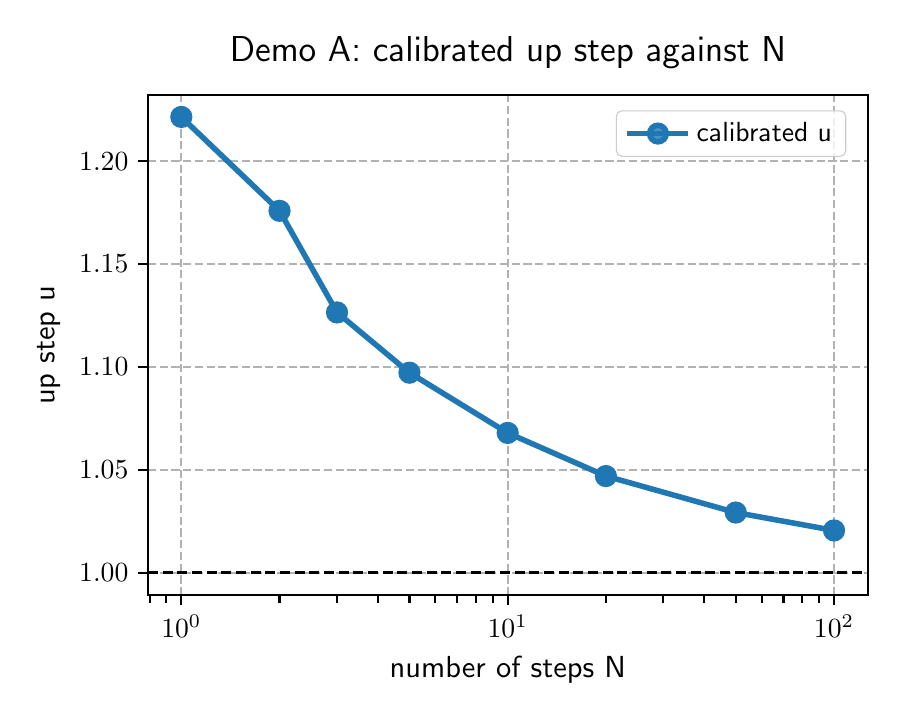
\begin{tikzpicture}
\begin{axis}[mpl, mplgrid, mplmark, width=3.6in, height=2.5in, xmode=log, xmin=0.79, xmax=127, ymin=0.989, ymax=1.232,
  ytick={1.00,1.05,1.10,1.15,1.20}, yticklabel style={/pgf/number format/fixed, /pgf/number format/precision=2, /pgf/number format/fixed zerofill},
  title={\fontsize{13}{15}\selectfont\sffamily Demo A: calibrated up step against N},
  xlabel={\fontsize{11}{13}\selectfont\sffamily number of steps N}, ylabel={\fontsize{11}{13}\selectfont\sffamily up step u},
  legend pos=north east, legend style={font=\fontsize{10}{12}\selectfont\sffamily}]
\addplot[tabblue, line width=2pt, mark=*, mark size=3pt, mark options={solid}] coordinates {(1,1.221464) (2,1.175830) (3,1.126435) (5,1.097162) (10,1.067895) (20,1.046925) (50,1.029196) (100,1.020503)};
\addlegendentry{calibrated u}
\addplot[black, line width=1pt, mpldash, forget plot] coordinates {(0.79,1.0) (127,1.0)};
\end{axis}
\end{tikzpicture}}\hfill
\resizebox{0.495\textwidth}{!}{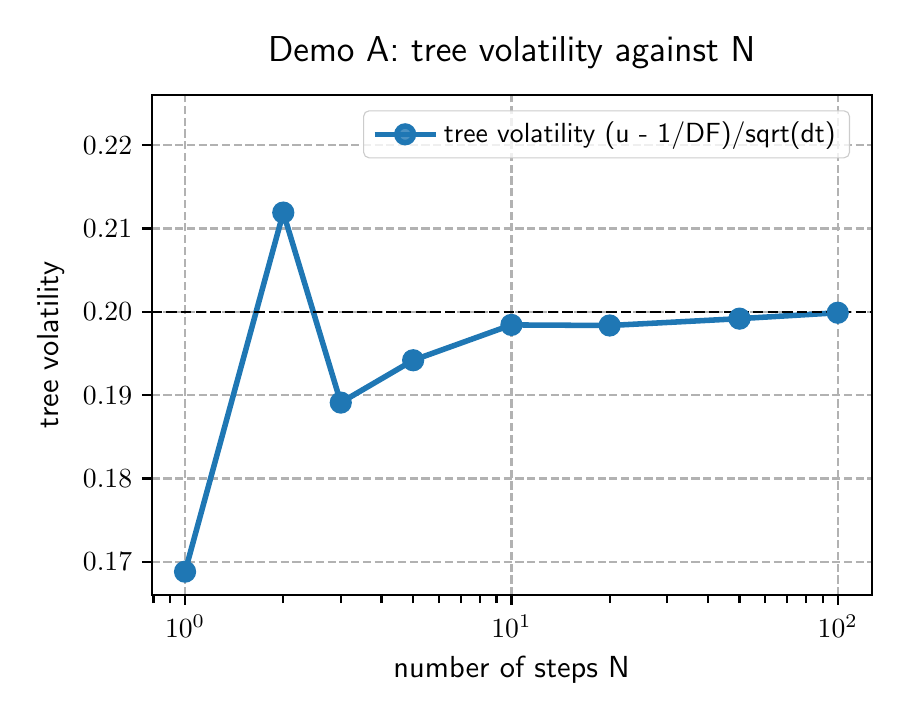
\begin{tikzpicture}
\begin{axis}[mpl, mplgrid, mplmark, width=3.6in, height=2.5in, xmode=log, xmin=0.79, xmax=127, ymin=0.166, ymax=0.226,
  ytick={0.17,0.18,0.19,0.20,0.21,0.22}, yticklabel style={/pgf/number format/fixed, /pgf/number format/precision=2, /pgf/number format/fixed zerofill},
  title={\fontsize{13}{15}\selectfont\sffamily Demo A: tree volatility against N},
  xlabel={\fontsize{11}{13}\selectfont\sffamily number of steps N}, ylabel={\fontsize{11}{13}\selectfont\sffamily tree volatility},
  legend pos=north east, legend style={font=\fontsize{10}{12}\selectfont\sffamily}]
\addplot[tabblue, line width=2pt, mark=*, mark size=3pt, mark options={solid}] coordinates {(1,0.16883) (2,0.21192) (3,0.18912) (5,0.19420) (10,0.19844) (20,0.19837) (50,0.19919) (100,0.19990)};
\addlegendentry{tree volatility (u - 1/DF)/sqrt(dt)}
\addplot[black, line width=1pt, mpldash, forget plot] coordinates {(0.79,0.2) (127,0.2)};
\end{axis}
\end{tikzpicture}}
\captionof{figure}{Demo A plots (Q4): calibrated $u$ (left, dashed line $u=1$) and tree volatility (right, dashed line $\sigma=0.2$) against $N$, logarithmic axis.}\label{fig:A}
\end{minipage}

\par\medskip\noindent\textbf{Reading.}
\begin{itemize}
\item Every calibration passes Step 5: $|V(u)-V^*|\le7.1\cdot10^{-16}$ in the output.
\item $u$ decreases from $1.221464$ ($N=1$) to $1.020503$ ($N=100$), towards $1$: $1/DF=0.95^{-1/N}\to1$ and the step size $h=u-1/DF$ goes from $0.168832$ to $0.019990\approx0.2\sqrt{1/100}$ (Lemma~2: $h$ is the standard deviation of one step, like $\sigma\sqrt{\Delta t}$).
\item The tree volatility tends to $0.2$ ($0.1999$ for $N=100$), the $\sigma$ that produced $V^*$: the calibrated tree recovers the Black--Scholes volatility, as expected from (C1) of Part~1. For small $N$ it oscillates ($0.1688$, $0.2119$, $0.1891$ for $N=1,2,3$).
\end{itemize}

\ansbox{\textbf{Q2 (Demo A).} For the same contract, \texttt{calibrate} works for every $N$ with the scaled $DF=0.95^{1/N}$ (Table~\ref{tab:A}). The calibrated up step decreases to $1$, its step size shrinks like $\sqrt{\Delta t}$, and the tree volatility $(u-1/DF)/\sqrt{\Delta t}$ converges to $\sigma=0.2$ of the market price ($0.1688$ for $N=1$, $0.1999$ for $N=100$; Figure~\ref{fig:A}).}

% ============================================================================ Q3
\subhead{Q3 --- Demo B: one-step tree for several contracts.}
$S_0=1$, flat rate ($DF_1=0.95$, so $DF=0.95^{T}$ for one step), $T\in\{0.25,0.5,1,2\}$, $K\in\{0.8,0.9,1.0,1.1,1.2\}$; each market price is the Black--Scholes price with $\sigma=0.2$. The code also checks every $u$ against \texttt{scipy.optimize.brentq}, another root solver (\texttt{assert}). Calibrating a one-step tree to a single European contract is what the earlier edition of the lecture~[2] describes.

\begin{center}
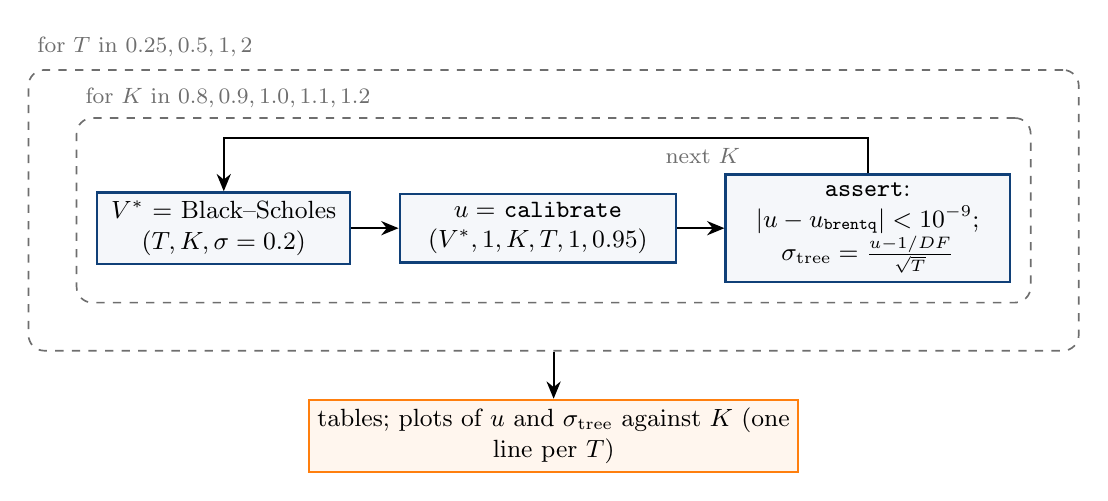
\begin{tikzpicture}[node distance=5mm and 6mm]
\node[fcbox, text width=3.0cm] (a) {$V^*$ = Black--Scholes\\ $(T,K,\sigma=0.2)$};
\node[fcbox, text width=3.3cm, right=of a] (b) {$u=$ \texttt{calibrate}\\ $(V^*,1,K,T,1,0.95)$};
\node[fcbox, text width=3.4cm, right=of b] (c) {\texttt{assert}: $|u-u_{\texttt{brentq}}|<10^{-9}$;\\ $\sigma_{\text{tree}}=\frac{u-1/DF}{\sqrt T}$};
\coordinate (top) at ($(b.north)+(0,7mm)$);
\node[fcloop, fit=(a)(b)(c)(top), label={[fclab, anchor=south west]north west:for $K$ in $0.8,0.9,1.0,1.1,1.2$}] (L1) {};
\node[fcloop, inner sep=6mm, fit=(L1), label={[fclab, anchor=south west, yshift=1pt]north west:for $T$ in $0.25,0.5,1,2$}] (L2) {};
\node[fcplot, text width=6cm, below=6mm of L2] (p) {tables; plots of $u$ and $\sigma_{\text{tree}}$ against $K$ (one line per $T$)};
\draw[fcarr] (a) -- (b); \draw[fcarr] (b) -- (c);
\draw[fcarr] (c.north) |- node[pos=0.75, below, fclab] {next $K$} (top) -| (a.north);
\draw[fcarr] (L2) -- (p);
\end{tikzpicture}
\captionof{figure}{Flowchart of Demo B.}\label{fig:fB}
\end{center}

\par\smallskip\noindent\begin{minipage}{\linewidth}\begin{lstlisting}[style=pysmall,title={Demo B (\texttt{demo\_B.py})}]
# Demo B: one-step tree, several contracts (expiries T, strikes K), flat rate (yearly DF = 0.95)
import numpy as np
from scipy.optimize import brentq
from plotter import my_plotter
from hw1_call import black_scholes_eur_call
from bg_functions import balanced_tree_call_price
from calibrator import calibrate, tree_vol

spot, df_annual, sigma = 1.0, 0.95, 0.2
r = -np.log(df_annual)
expiries = [0.25, 0.5, 1.0, 2.0]
strikes = [0.8, 0.9, 1.0, 1.1, 1.2]
u_table, vol_table = [], []
for T in expiries:
    u_row, vol_row = [], []
    for K in strikes:
        price = black_scholes_eur_call(r=r, T=T, S0=spot, sigma=sigma, K=K)[0]
        u = calibrate(price, spot, K, T, 1, df_annual)       # one step: DF = df_annual**T
        DF = df_annual ** T
        u_brentq = brentq(lambda x: balanced_tree_call_price(spot, K, T, 1, df_annual, x)
                          - price, 1 / DF + 1e-10, 2 / DF - 1e-10, xtol=1e-14)
        assert abs(u - u_brentq) < 1e-9                          # another root solver
        u_row.append(u)
        vol_row.append(tree_vol(u, T, 1, df_annual))
    u_table.append(u_row)
    vol_table.append(vol_row)
    print(f"T = {T:4.2f}  u = " + "  ".join(f"{u:.4f}" for u in u_row)
          + "   tree vol = " + "  ".join(f"{v:.3f}" for v in vol_row))

common = {"grid": True, "title_fontsize": 13, "label_fontsize": 11, "legend_fontsize": 10,
          "linewidth": 2, "markers": "o", "hline": None, "show": False}
names = [f"T = {T}" for T in expiries]
my_plotter(strikes, u_table, names=names,
           layout={**common, "title": "Demo B: one-step tree, calibrated up step",
                   "x_label": "strike K", "y_label": "up step u", "legend_loc": "upper center",
                   "save_path": "figures/demoB_u.pdf"})
my_plotter(strikes, vol_table, names=names,
           layout={**common, "title": "Demo B: one-step tree, tree volatility",
                   "x_label": "strike K", "y_label": "tree volatility",
                   "save_path": "figures/demoB_vol.pdf"})
\end{lstlisting}
\begin{lstlisting}[style=out,title={output (\texttt{demo\_B.out}; per row: $u$ for $K = 0.8, \dots, 1.2$, then the tree volatilities)}]
T = 0.25  u = 1.2264  1.1369  1.0938  1.1243  1.2041   tree vol = 0.427  0.248  0.162  0.223  0.382
T = 0.50  u = 1.2560  1.1779  1.1421  1.1600  1.2212   tree vol = 0.325  0.215  0.164  0.190  0.276
T = 1.00  u = 1.3195  1.2533  1.2215  1.2282  1.2691   tree vol = 0.267  0.201  0.169  0.176  0.216
T = 2.00  u = 1.4488  1.3916  1.3604  1.3564  1.3778   tree vol = 0.241  0.201  0.178  0.176  0.191
\end{lstlisting}\end{minipage}\par\smallskip

\noindent The \texttt{assert} did not stop the run, so \texttt{calibrate} equals the \texttt{brentq} solution to $10^{-9}$ in all $20$ cases. Table~\ref{tab:Bp} shows that every market price is attainable (Step 2); Table~\ref{tab:Bu} collects the output.

\begin{center}
\small
\begin{tabular}{cc*{5}{c}}
\toprule
$T$ & & $K=0.8$ & $K=0.9$ & $K=1.0$ & $K=1.1$ & $K=1.2$\\
\midrule
\multirow{3}{*}{0.25} & $V_{\min}$ & 0.2102 & 0.1115 & 0.0127 & 0.0000 & 0.0000\\
 & $V^*$ & \textbf{0.210466} & \textbf{0.116951} & \textbf{0.046319} & \textbf{0.011978} & \textbf{0.002013}\\
 & $V_{\max}$ & 0.6051 & 0.5557 & 0.5064 & 0.4570 & 0.4076\\
\midrule
\multirow{3}{*}{0.50} & $V_{\min}$ & 0.2203 & 0.1228 & 0.0253 & 0.0000 & 0.0000\\
 & $V^*$ & \textbf{0.222227} & \textbf{0.135441} & \textbf{0.069230} & \textbf{0.029263} & \textbf{0.010316}\\
 & $V_{\max}$ & 0.6101 & 0.5614 & 0.5127 & 0.4639 & 0.4152\\
\midrule
\multirow{3}{*}{1.00} & $V_{\min}$ & 0.2400 & 0.1450 & 0.0500 & 0.0000 & 0.0000\\
 & $V^*$ & \textbf{0.246771} & \textbf{0.167826} & \textbf{0.105195} & \textbf{0.060906} & \textbf{0.032805}\\
 & $V_{\max}$ & 0.6200 & 0.5725 & 0.5250 & 0.4775 & 0.4300\\
\midrule
\multirow{3}{*}{2.00} & $V_{\min}$ & 0.2780 & 0.1878 & 0.0975 & 0.0072 & 0.0000\\
 & $V^*$ & \textbf{0.292778} & \textbf{0.221853} & \textbf{0.162637} & \textbf{0.115717} & \textbf{0.080220}\\
 & $V_{\max}$ & 0.6390 & 0.5939 & 0.5487 & 0.5036 & 0.4585\\
\bottomrule
\end{tabular}
\captionof{table}{Demo B: market price $V^*$ (bold) between $V_{\min}$ and $V_{\max}$ of Step 2 (from \texttt{outputs.txt}).}\label{tab:Bp}
\end{center}

\begin{center}
\small
\begin{tabular}{c*{5}{c}c*{5}{c}}
\toprule
 & \multicolumn{5}{c}{calibrated up step $u$} & & \multicolumn{5}{c}{tree volatility $\sigma_{\text{tree}}=(u-1/DF)/\sqrt T$}\\
\cmidrule(lr){2-6}\cmidrule(lr){8-12}
$T$ & $0.8$ & $0.9$ & $1.0$ & $1.1$ & $1.2$ & & $0.8$ & $0.9$ & $1.0$ & $1.1$ & $1.2$\\
\midrule
0.25 & 1.2264 & 1.1369 & 1.0938 & 1.1243 & 1.2041 & & 0.427 & 0.248 & 0.162 & 0.223 & 0.382\\
0.50 & 1.2560 & 1.1779 & 1.1421 & 1.1600 & 1.2212 & & 0.325 & 0.215 & 0.164 & 0.190 & 0.276\\
1.00 & 1.3195 & 1.2533 & 1.2215 & 1.2282 & 1.2691 & & 0.267 & 0.201 & 0.169 & 0.176 & 0.216\\
2.00 & 1.4488 & 1.3916 & 1.3604 & 1.3564 & 1.3778 & & 0.241 & 0.201 & 0.178 & 0.176 & 0.191\\
\bottomrule
\end{tabular}
\captionof{table}{Demo B: $u$ and $\sigma_{\text{tree}}$ by expiry $T$ (rows) and strike $K$ (columns), from \texttt{demo\_B.out}.}\label{tab:Bu}
\end{center}

\noindent\begin{minipage}{\linewidth}
\resizebox{0.495\textwidth}{!}{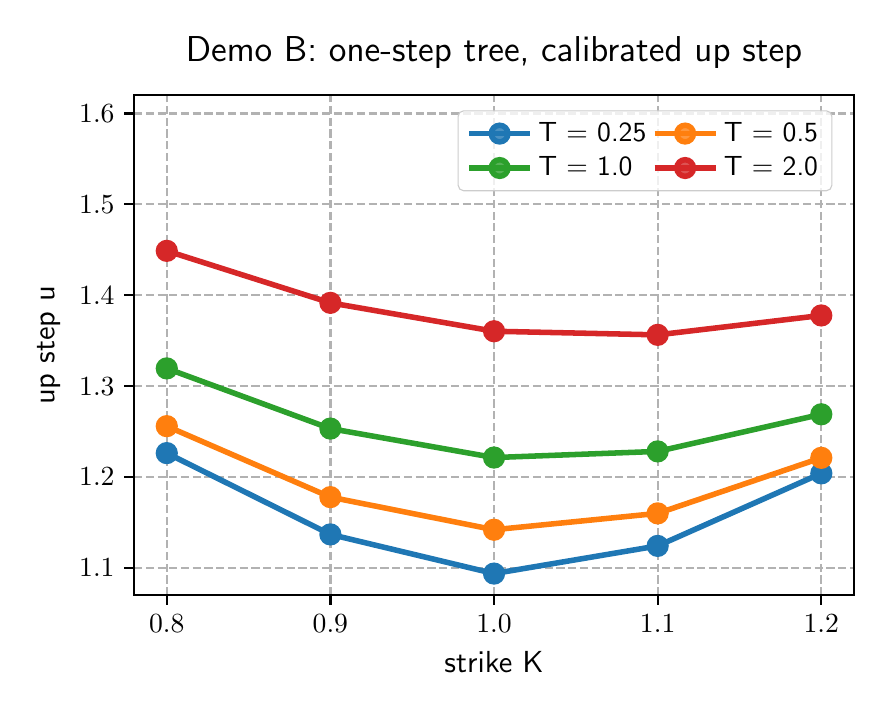
\begin{tikzpicture}
\begin{axis}[mpl, mplgrid, mplmark, width=3.6in, height=2.5in, xmin=0.78, xmax=1.22, ymin=1.07, ymax=1.62,
  xtick={0.8,0.9,1.0,1.1,1.2}, ytick={1.1,1.2,1.3,1.4,1.5,1.6},
  xticklabel style={/pgf/number format/fixed, /pgf/number format/precision=1, /pgf/number format/fixed zerofill},
  yticklabel style={/pgf/number format/fixed, /pgf/number format/precision=1, /pgf/number format/fixed zerofill},
  title={\fontsize{13}{15}\selectfont\sffamily Demo B: one-step tree, calibrated up step},
  xlabel={\fontsize{11}{13}\selectfont\sffamily strike K}, ylabel={\fontsize{11}{13}\selectfont\sffamily up step u},
  legend pos=north east, legend columns=2, legend style={font=\fontsize{10}{12}\selectfont\sffamily}]
\addplot[tabblue, line width=2pt, mark=*, mark size=3pt] coordinates {(0.8,1.22636) (0.9,1.13692) (1.0,1.09383) (1.1,1.12427) (1.2,1.20408)};
\addlegendentry{T = 0.25}
\addplot[taborange, line width=2pt, mark=*, mark size=3pt] coordinates {(0.8,1.25600) (0.9,1.17792) (1.0,1.14206) (1.1,1.16005) (1.2,1.22117)};
\addlegendentry{T = 0.5}
\addplot[tabgreen, line width=2pt, mark=*, mark size=3pt] coordinates {(0.8,1.31952) (0.9,1.25332) (1.0,1.22146) (1.1,1.22822) (1.2,1.26906)};
\addlegendentry{T = 1.0}
\addplot[tabred, line width=2pt, mark=*, mark size=3pt] coordinates {(0.8,1.44882) (0.9,1.39164) (1.0,1.36041) (1.1,1.35644) (1.2,1.37777)};
\addlegendentry{T = 2.0}
\end{axis}
\end{tikzpicture}}\hfill
\resizebox{0.495\textwidth}{!}{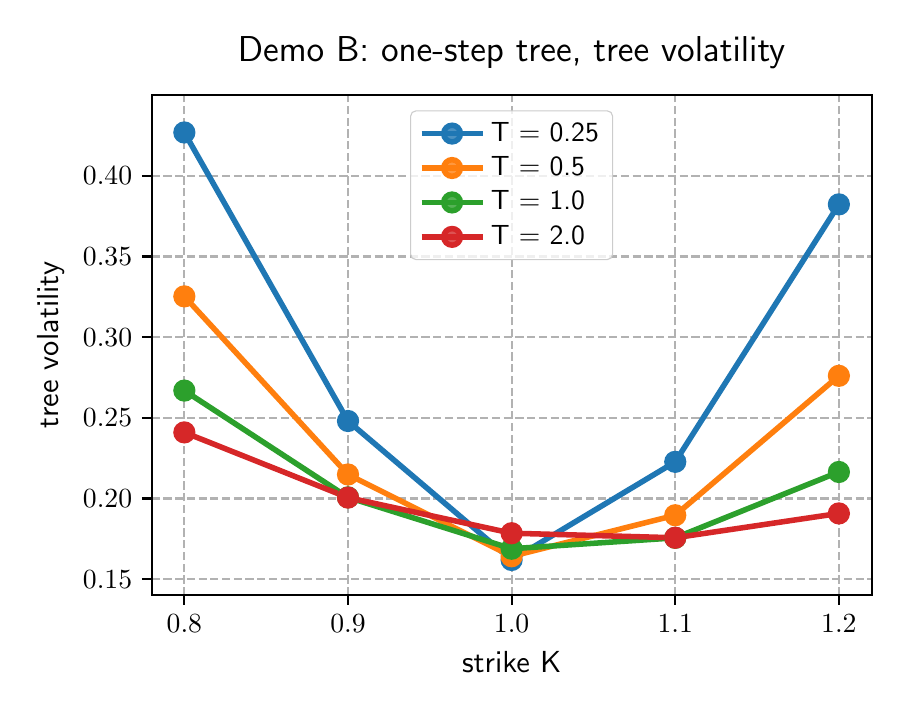
\begin{tikzpicture}
\begin{axis}[mpl, mplgrid, mplmark, width=3.6in, height=2.5in, xmin=0.78, xmax=1.22, ymin=0.14, ymax=0.45,
  xtick={0.8,0.9,1.0,1.1,1.2}, ytick={0.15,0.20,0.25,0.30,0.35,0.40},
  xticklabel style={/pgf/number format/fixed, /pgf/number format/precision=1, /pgf/number format/fixed zerofill},
  yticklabel style={/pgf/number format/fixed, /pgf/number format/precision=2, /pgf/number format/fixed zerofill},
  title={\fontsize{13}{15}\selectfont\sffamily Demo B: one-step tree, tree volatility},
  xlabel={\fontsize{11}{13}\selectfont\sffamily strike K}, ylabel={\fontsize{11}{13}\selectfont\sffamily tree volatility},
  legend style={at={(0.5,0.97)}, anchor=north, font=\fontsize{10}{12}\selectfont\sffamily}]
\addplot[tabblue, line width=2pt, mark=*, mark size=3pt] coordinates {(0.8,0.42692) (0.9,0.24803) (1.0,0.16186) (1.1,0.22272) (1.2,0.38234)};
\addlegendentry{T = 0.25}
\addplot[taborange, line width=2pt, mark=*, mark size=3pt] coordinates {(0.8,0.32530) (0.9,0.21488) (1.0,0.16416) (1.1,0.18960) (1.2,0.27604)};
\addlegendentry{T = 0.5}
\addplot[tabgreen, line width=2pt, mark=*, mark size=3pt] coordinates {(0.8,0.26689) (0.9,0.20069) (1.0,0.16883) (1.1,0.17559) (1.2,0.21643)};
\addlegendentry{T = 1.0}
\addplot[tabred, line width=2pt, mark=*, mark size=3pt] coordinates {(0.8,0.24097) (0.9,0.20054) (1.0,0.17846) (1.1,0.17565) (1.2,0.19073)};
\addlegendentry{T = 2.0}
\end{axis}
\end{tikzpicture}}
\captionof{figure}{Demo B plots (Q4): calibrated $u$ (left) and tree volatility (right) against the strike, one line per expiry.}\label{fig:B}
\end{minipage}

\par\medskip\noindent\textbf{Reading.}
\begin{itemize}
\item Every price is attainable (Table~\ref{tab:Bp}); the closest case is $T=0.25$, $K=0.8$: $V^*=0.210466$ against $V_{\min}=0.2102$.
\item For each strike, $u$ grows with $T$ (e.g.\ $K=1.0$: $1.0938$, $1.1421$, $1.2215$, $1.3604$): one step now lasts $T$ years, and by Lemma~2 $u=1/DF+\sigma_{\text{tree}}\sqrt T$.
\item The tree volatility is not flat in $K$: it is smallest near the money ($0.162$ at $T=0.25$, $K=1.0$; for $T=2$ at $K=1.1$, near the mean $S_0/DF=1/0.95^2\approx1.108$ of the leaves, Lemma~2) and larger in the wings ($0.427$ at $T=0.25$, $K=0.8$). A one-step tree has only two leaves and cannot reproduce the Black--Scholes distribution, so each strike needs its own step.
\end{itemize}

\ansbox{\textbf{Q3 (Demo B).} The one-step tree can be calibrated to all $20$ contracts (flat rate, $DF=0.95^T$), and \texttt{calibrate} agrees with \texttt{brentq} to $10^{-9}$. The calibrated $u$ grows with the expiry (Table~\ref{tab:Bu}); the tree volatility depends on the strike, smallest near the money and larger in the wings (Figure~\ref{fig:B}): one step cannot match Black--Scholes for all strikes with one $u$.}

% ============================================================================ Q4 trees
\subhead{Q4 --- the calibrated trees.}
To see how the calibrated model works, we draw the trees of the lecture code for the contract of Demo A ($S_0=K=1$, $T=1$, $DF_1=0.95$, $V^*=0.105195$): the spot tree (cell 5) and the price tree (cell 8) with the calibrated $u$. $N=2$ and $N=5$: every node; $N=50$: all $1326$ nodes, labels on the first, middle and last level (bottom, middle and top node). $V$ is the value returned by \texttt{create\_discounted\_price\_tree}: discounted to $t=0$ (Definition~1, cell 8), so the root is the price.

\begin{center}
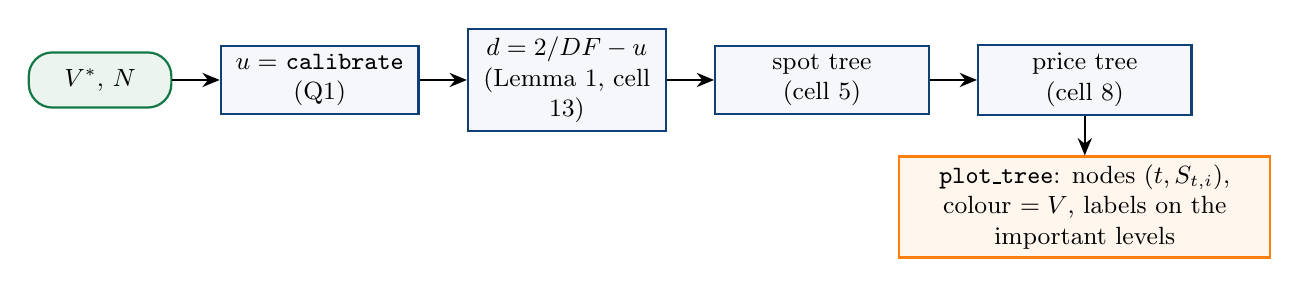
\begin{tikzpicture}[node distance=5mm and 6mm]
\node[fcterm, text width=1.6cm] (a) {$V^*$, $N$};
\node[fcbox, text width=2.3cm, right=of a] (b) {$u=$ \texttt{calibrate} (Q1)};
\node[fcbox, text width=2.3cm, right=of b] (c) {$d=2/DF-u$\\ (Lemma~1, cell 13)};
\node[fcbox, text width=2.5cm, right=of c] (d) {spot tree\\ (cell 5)};
\node[fcbox, text width=2.5cm, right=of d] (e) {price tree\\ (cell 8)};
\node[fcplot, text width=4.5cm, below=of e] (f) {\texttt{plot\_tree}: nodes $(t,S_{t,i})$, colour $=V$, labels on the important levels};
\draw[fcarr] (a) -- (b); \draw[fcarr] (b) -- (c); \draw[fcarr] (c) -- (d); \draw[fcarr] (d) -- (e); \draw[fcarr] (e) -- (f);
\end{tikzpicture}
\captionof{figure}{Flowchart of Q4 (file \texttt{tree\_plot.py}).}\label{fig:fT}
\end{center}

\par\smallskip\noindent\begin{minipage}{\linewidth}\begin{lstlisting}[style=pysmall,title={new code (\texttt{tree\_plot.py})}]
"""Homework 2, part 2 (Q4): pictures of the calibrated balanced trees.

calibrated_trees(...) calibrates u with calibrate (Q1) and builds the two trees of the lecture
code: the spot tree (create_spot_tree) and the price tree (create_discounted_price_tree).
plot_tree(...) draws them: x = time step t, y = spot S_{t,i}, colour = value of the node as
returned by create_discounted_price_tree (discounted to t = 0; the root is the price).
Small trees: every node is labelled. Large trees: all nodes are drawn, labels only on the
important levels (first, second, middle, last) and on the top, middle and bottom node.
"""
import matplotlib.pyplot as plt
import numpy as np
from matplotlib.collections import LineCollection

from calibrator import calibrate
from prof_tree import calcBalancedDownStep, create_discounted_price_tree, create_spot_tree


def calibrated_trees(price: float, spot: float, strike: float, maturity: float, steps: int,
                     df_annual: float):
    """Return (u, d, DF, spot_tree, price_tree) of the balanced tree calibrated to price."""
    u = calibrate(price, spot, strike, maturity, steps, df_annual)
    discount_factor = df_annual ** (maturity / steps)              # flat rate (Definition 3)
    d = calcBalancedDownStep(u, discount_factor)                   # lecture, cell 13
    spot_tree = create_spot_tree(spot, u, d, steps)                # lecture, cell 5
    price_tree = create_discounted_price_tree(spot_tree, discount_factor, strike)   # cell 8
    return u, d, discount_factor, spot_tree, price_tree


def important_nodes(level: int) -> list[int]:
    """Indices i of the nodes of level t to label: all of them if few, else bottom/middle/top."""
    return list(range(level + 1)) if level <= 5 else sorted({0, level // 2, level})


def plot_tree(spot_tree, price_tree, strike=None, label_levels=None, title=None, ax=None,
              fontsize=8, logy=None):
    """Draw a spot tree with its price tree. Returns (fig, ax)."""
    steps = len(spot_tree) - 1
    if label_levels is None:
        label_levels = range(steps + 1) if steps <= 5 else sorted({0, steps // 2, steps})
    if logy is None:
        logy = steps > 5                     # log scale: the large tree looks symmetric
    if ax is None:
        ax = plt.subplots(figsize=(9, 5))[1]
    fig = ax.figure
    # edges: node (t, i) -> down child (t+1, i) and up child (t+1, i+1)
    segments = [[(t, spot_tree[t][i]), (t + 1, spot_tree[t + 1][j])]
                for t in range(steps) for i in range(t + 1) for j in (i, i + 1)]
    ax.add_collection(LineCollection(segments, colors="0.75", linewidths=0.6, zorder=1))
    # nodes, coloured by the value of the price tree
    xs = [t for t in range(steps + 1) for _ in spot_tree[t]]
    ys = [s for level in spot_tree for s in level]
    vs = [v for level in price_tree for v in level]
    size = 60 if steps <= 5 else max(4, 400 / steps)
    points = ax.scatter(xs, ys, c=vs, cmap="viridis", s=size, zorder=2)
    fig.colorbar(points, ax=ax, label="node value (discounted to t = 0)")
    for t in label_levels:
        for i in important_nodes(t):
            ax.annotate(f"S={spot_tree[t][i]:.3f}\nV={price_tree[t][i]:.4f}",
                        (t, spot_tree[t][i]), textcoords="offset points", xytext=(4, 4),
                        fontsize=fontsize, zorder=3,
                        bbox={"boxstyle": "round,pad=0.15", "fc": "white", "alpha": 0.8, "lw": 0})
    if strike is not None:
        ax.axhline(strike, linestyle="--", color="tab:red", linewidth=1, label=f"strike K = {strike}")
        ax.legend(loc="upper left", fontsize=fontsize + 1)
    if logy:
        ax.set_yscale("log")
        ticks = [2.0 ** k for k in range(-6, 7) if min(ys) <= 2.0 ** k <= max(ys)]
        ax.set_yticks(ticks, [f"{x:g}" for x in ticks])
        ax.minorticks_off()
    ax.set_xlabel("time step t")
    ax.set_ylabel("spot S" + (" (log scale)" if logy else ""))
    ax.set_xlim(-0.3, steps + 0.8 + 0.08 * steps)
    if title:
        ax.set_title(title)
    return fig, ax
\end{lstlisting}\end{minipage}\par\smallskip

\par\smallskip\noindent\begin{minipage}{\linewidth}\begin{lstlisting}[style=pysmall,title={run (\texttt{trees\_demo.py})}]
# Q4: the calibrated balanced trees of Demo A (S0 = K = 1, T = 1, yearly DF = 0.95), N = 2, 5, 50
import numpy as np
from hw1_call import black_scholes_eur_call
from tree_plot import calibrated_trees, important_nodes, plot_tree

spot, strike, maturity, df_annual = 1.0, 1.0, 1.0, 0.95
r = -np.log(df_annual)
target = black_scholes_eur_call(r=r, T=maturity, S0=spot, sigma=0.2, K=strike)[0]
print(f"target price: {target:.6f}")

for steps in [2, 5, 50]:
    u, d, DF, spot_tree, price_tree = calibrated_trees(target, spot, strike, maturity, steps,
                                                       df_annual)
    print(f"\nN = {steps}: u = {u:.6f}, d = {d:.6f}, DF = {DF:.6f}, "
          f"root value = {price_tree[0][0]:.6f}")
    for t in sorted({0, 1, steps // 2, steps}):
        nodes = [f"(S={spot_tree[t][i]:.4f}, V={price_tree[t][i]:.6f})" for i in important_nodes(t)]
        for k in range(0, len(nodes), 3):                    # at most 3 nodes per line
            print(f"  t = {t:2d}: " + "  ".join(nodes[k:k + 3]))
    # backward induction check at the root: V_0 = (V_up + V_down) / 2 (p_up = p_down = 1/2)
    print(f"  (V_up + V_down)/2 at t = 1: {(price_tree[1][0] + price_tree[1][1]) / 2:.6f}")
    plot_tree(spot_tree, price_tree, strike=strike,
              title=f"Calibrated balanced tree, N = {steps} (u = {u:.4f})")[0].savefig(
        f"figures/tree_N{steps}.pdf")
\end{lstlisting}
\begin{lstlisting}[style=out,title={output (\texttt{trees\_demo.out})}]
target price: 0.105195

N = 2: u = 1.175830, d = 0.876127, DF = 0.974679, root value = 0.105195
  t =  0: (S=1.0000, V=0.105195)
  t =  1: (S=0.8761, V=0.014334)  (S=1.1758, V=0.196057)
  t =  2: (S=0.7676, V=0.000000)  (S=1.0302, V=0.028667)  (S=1.3826, V=0.363447)
  (V_up + V_down)/2 at t = 1: 0.105195

N = 5: u = 1.097162, d = 0.923461, DF = 0.989794, root value = 0.105195
  t =  0: (S=1.0000, V=0.105195)
  t =  1: (S=0.9235, V=0.050070)  (S=1.0972, V=0.160320)
  t =  2: (S=0.8528, V=0.014997)  (S=1.0132, V=0.085144)  (S=1.2038, V=0.235497)
  t =  5: (S=0.6716, V=0.000000)  (S=0.7979, V=0.000000)  (S=0.9480, V=0.000000)
  t =  5: (S=1.1263, V=0.119973)  (S=1.3381, V=0.321234)  (S=1.5898, V=0.560351)
  (V_up + V_down)/2 at t = 1: 0.105195

N = 50: u = 1.029196, d = 0.972857, DF = 0.998975, root value = 0.105195
  t =  0: (S=1.0000, V=0.105195)
  t =  1: (S=0.9729, V=0.087210)  (S=1.0292, V=0.123180)
  t = 25: (S=0.5026, V=0.000000)  (S=0.9877, V=0.060739)  (S=2.0533, V=1.051299)
  t = 50: (S=0.2526, V=0.000000)  (S=1.0320, V=0.030390)  (S=4.2160, V=3.055198)
  (V_up + V_down)/2 at t = 1: 0.105195
\end{lstlisting}\end{minipage}\par\smallskip

\begin{center}
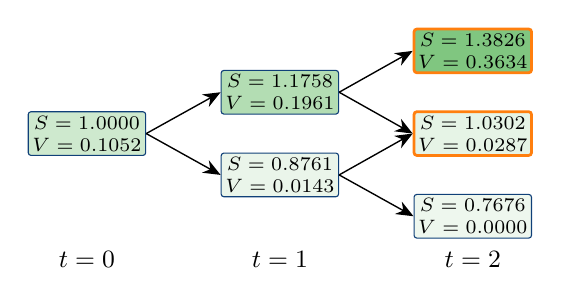
\begin{tikzpicture}
\node[draw=DefBlue, fill=tabgreen!23, rounded corners=1pt, align=center, font=\scriptsize, inner sep=1.5pt] (n0x0) at (0.00,0.000) {$S=1.0000$\\ $V=0.1052$};
\node[draw=DefBlue, fill=tabgreen!10, rounded corners=1pt, align=center, font=\scriptsize, inner sep=1.5pt] (n1x0) at (2.45,-0.525) {$S=0.8761$\\ $V=0.0143$};
\node[draw=DefBlue, fill=tabgreen!36, rounded corners=1pt, align=center, font=\scriptsize, inner sep=1.5pt] (n1x1) at (2.45,0.525) {$S=1.1758$\\ $V=0.1961$};
\node[draw=DefBlue, fill=tabgreen!8, rounded corners=1pt, align=center, font=\scriptsize, inner sep=1.5pt] (n2x0) at (4.90,-1.050) {$S=0.7676$\\ $V=0.0000$};
\node[draw=taborange, line width=1pt, fill=tabgreen!12, rounded corners=1pt, align=center, font=\scriptsize, inner sep=1.5pt] (n2x1) at (4.90,0.000) {$S=1.0302$\\ $V=0.0287$};
\node[draw=taborange, line width=1pt, fill=tabgreen!60, rounded corners=1pt, align=center, font=\scriptsize, inner sep=1.5pt] (n2x2) at (4.90,1.050) {$S=1.3826$\\ $V=0.3634$};
\draw[fcarr, line width=0.5pt] (n0x0.east) -- (n1x0.west);
\draw[fcarr, line width=0.5pt] (n0x0.east) -- (n1x1.west);
\draw[fcarr, line width=0.5pt] (n1x0.east) -- (n2x0.west);
\draw[fcarr, line width=0.5pt] (n1x0.east) -- (n2x1.west);
\draw[fcarr, line width=0.5pt] (n1x1.east) -- (n2x1.west);
\draw[fcarr, line width=0.5pt] (n1x1.east) -- (n2x2.west);
\node[font=\small] at (0,-1.6) {$t=0$}; \node[font=\small] at (2.45,-1.6) {$t=1$}; \node[font=\small] at (4.9,-1.6) {$t=2$};
\end{tikzpicture}
\captionof{figure}{Calibrated tree, $N=2$ ($u=1.175830$, $d=0.876127$, $DF=0.974679$). Up moves go up. Colour: value $V$; orange border: leaf above $K$.}\label{fig:T2}
\end{center}

\begin{center}
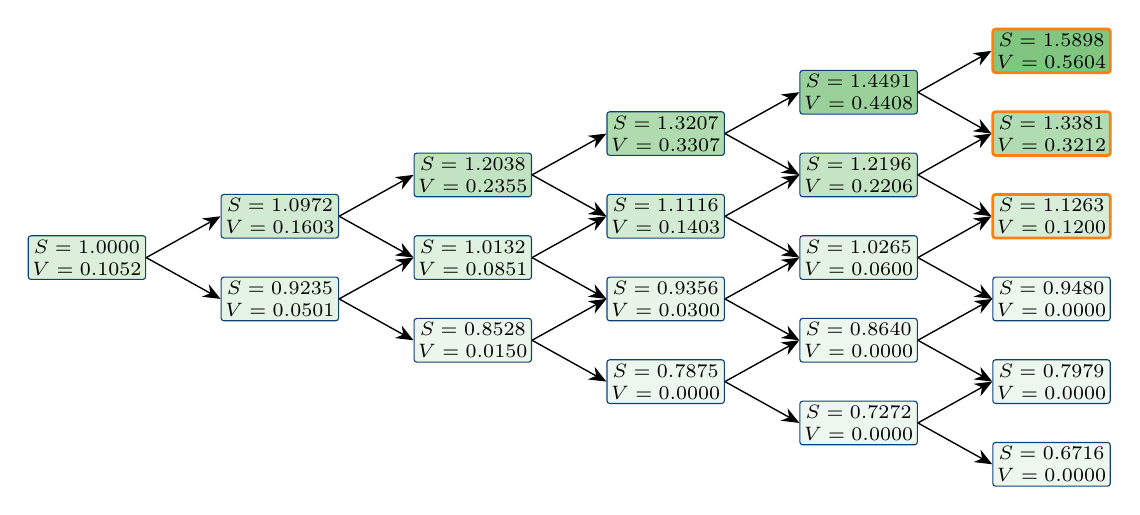
\begin{tikzpicture}
\node[draw=DefBlue, fill=tabgreen!17, rounded corners=1pt, align=center, font=\scriptsize, inner sep=1.5pt] (n0x0) at (0.00,0.000) {$S=1.0000$\\ $V=0.1052$};
\node[draw=DefBlue, fill=tabgreen!12, rounded corners=1pt, align=center, font=\scriptsize, inner sep=1.5pt] (n1x0) at (2.45,-0.525) {$S=0.9235$\\ $V=0.0501$};
\node[draw=DefBlue, fill=tabgreen!22, rounded corners=1pt, align=center, font=\scriptsize, inner sep=1.5pt] (n1x1) at (2.45,0.525) {$S=1.0972$\\ $V=0.1603$};
\node[draw=DefBlue, fill=tabgreen!9, rounded corners=1pt, align=center, font=\scriptsize, inner sep=1.5pt] (n2x0) at (4.90,-1.050) {$S=0.8528$\\ $V=0.0150$};
\node[draw=DefBlue, fill=tabgreen!15, rounded corners=1pt, align=center, font=\scriptsize, inner sep=1.5pt] (n2x1) at (4.90,0.000) {$S=1.0132$\\ $V=0.0851$};
\node[draw=DefBlue, fill=tabgreen!29, rounded corners=1pt, align=center, font=\scriptsize, inner sep=1.5pt] (n2x2) at (4.90,1.050) {$S=1.2038$\\ $V=0.2355$};
\node[draw=DefBlue, fill=tabgreen!8, rounded corners=1pt, align=center, font=\scriptsize, inner sep=1.5pt] (n3x0) at (7.35,-1.575) {$S=0.7875$\\ $V=0.0000$};
\node[draw=DefBlue, fill=tabgreen!10, rounded corners=1pt, align=center, font=\scriptsize, inner sep=1.5pt] (n3x1) at (7.35,-0.525) {$S=0.9356$\\ $V=0.0300$};
\node[draw=DefBlue, fill=tabgreen!21, rounded corners=1pt, align=center, font=\scriptsize, inner sep=1.5pt] (n3x2) at (7.35,0.525) {$S=1.1116$\\ $V=0.1403$};
\node[draw=DefBlue, fill=tabgreen!38, rounded corners=1pt, align=center, font=\scriptsize, inner sep=1.5pt] (n3x3) at (7.35,1.575) {$S=1.3207$\\ $V=0.3307$};
\node[draw=DefBlue, fill=tabgreen!8, rounded corners=1pt, align=center, font=\scriptsize, inner sep=1.5pt] (n4x0) at (9.80,-2.100) {$S=0.7272$\\ $V=0.0000$};
\node[draw=DefBlue, fill=tabgreen!8, rounded corners=1pt, align=center, font=\scriptsize, inner sep=1.5pt] (n4x1) at (9.80,-1.050) {$S=0.8640$\\ $V=0.0000$};
\node[draw=DefBlue, fill=tabgreen!13, rounded corners=1pt, align=center, font=\scriptsize, inner sep=1.5pt] (n4x2) at (9.80,0.000) {$S=1.0265$\\ $V=0.0600$};
\node[draw=DefBlue, fill=tabgreen!28, rounded corners=1pt, align=center, font=\scriptsize, inner sep=1.5pt] (n4x3) at (9.80,1.050) {$S=1.2196$\\ $V=0.2206$};
\node[draw=DefBlue, fill=tabgreen!48, rounded corners=1pt, align=center, font=\scriptsize, inner sep=1.5pt] (n4x4) at (9.80,2.100) {$S=1.4491$\\ $V=0.4408$};
\node[draw=DefBlue, fill=tabgreen!8, rounded corners=1pt, align=center, font=\scriptsize, inner sep=1.5pt] (n5x0) at (12.25,-2.625) {$S=0.6716$\\ $V=0.0000$};
\node[draw=DefBlue, fill=tabgreen!8, rounded corners=1pt, align=center, font=\scriptsize, inner sep=1.5pt] (n5x1) at (12.25,-1.575) {$S=0.7979$\\ $V=0.0000$};
\node[draw=DefBlue, fill=tabgreen!8, rounded corners=1pt, align=center, font=\scriptsize, inner sep=1.5pt] (n5x2) at (12.25,-0.525) {$S=0.9480$\\ $V=0.0000$};
\node[draw=taborange, line width=1pt, fill=tabgreen!19, rounded corners=1pt, align=center, font=\scriptsize, inner sep=1.5pt] (n5x3) at (12.25,0.525) {$S=1.1263$\\ $V=0.1200$};
\node[draw=taborange, line width=1pt, fill=tabgreen!37, rounded corners=1pt, align=center, font=\scriptsize, inner sep=1.5pt] (n5x4) at (12.25,1.575) {$S=1.3381$\\ $V=0.3212$};
\node[draw=taborange, line width=1pt, fill=tabgreen!60, rounded corners=1pt, align=center, font=\scriptsize, inner sep=1.5pt] (n5x5) at (12.25,2.625) {$S=1.5898$\\ $V=0.5604$};
\draw[fcarr, line width=0.5pt] (n0x0.east) -- (n1x0.west);
\draw[fcarr, line width=0.5pt] (n0x0.east) -- (n1x1.west);
\draw[fcarr, line width=0.5pt] (n1x0.east) -- (n2x0.west);
\draw[fcarr, line width=0.5pt] (n1x0.east) -- (n2x1.west);
\draw[fcarr, line width=0.5pt] (n1x1.east) -- (n2x1.west);
\draw[fcarr, line width=0.5pt] (n1x1.east) -- (n2x2.west);
\draw[fcarr, line width=0.5pt] (n2x0.east) -- (n3x0.west);
\draw[fcarr, line width=0.5pt] (n2x0.east) -- (n3x1.west);
\draw[fcarr, line width=0.5pt] (n2x1.east) -- (n3x1.west);
\draw[fcarr, line width=0.5pt] (n2x1.east) -- (n3x2.west);
\draw[fcarr, line width=0.5pt] (n2x2.east) -- (n3x2.west);
\draw[fcarr, line width=0.5pt] (n2x2.east) -- (n3x3.west);
\draw[fcarr, line width=0.5pt] (n3x0.east) -- (n4x0.west);
\draw[fcarr, line width=0.5pt] (n3x0.east) -- (n4x1.west);
\draw[fcarr, line width=0.5pt] (n3x1.east) -- (n4x1.west);
\draw[fcarr, line width=0.5pt] (n3x1.east) -- (n4x2.west);
\draw[fcarr, line width=0.5pt] (n3x2.east) -- (n4x2.west);
\draw[fcarr, line width=0.5pt] (n3x2.east) -- (n4x3.west);
\draw[fcarr, line width=0.5pt] (n3x3.east) -- (n4x3.west);
\draw[fcarr, line width=0.5pt] (n3x3.east) -- (n4x4.west);
\draw[fcarr, line width=0.5pt] (n4x0.east) -- (n5x0.west);
\draw[fcarr, line width=0.5pt] (n4x0.east) -- (n5x1.west);
\draw[fcarr, line width=0.5pt] (n4x1.east) -- (n5x1.west);
\draw[fcarr, line width=0.5pt] (n4x1.east) -- (n5x2.west);
\draw[fcarr, line width=0.5pt] (n4x2.east) -- (n5x2.west);
\draw[fcarr, line width=0.5pt] (n4x2.east) -- (n5x3.west);
\draw[fcarr, line width=0.5pt] (n4x3.east) -- (n5x3.west);
\draw[fcarr, line width=0.5pt] (n4x3.east) -- (n5x4.west);
\draw[fcarr, line width=0.5pt] (n4x4.east) -- (n5x4.west);
\draw[fcarr, line width=0.5pt] (n4x4.east) -- (n5x5.west);
\end{tikzpicture}
\captionof{figure}{Calibrated tree, $N=5$ ($u=1.097162$, $d=0.923461$, $DF=0.989794$); from $t=0$ (left) to $t=5$ (right).}\label{fig:T5}
\end{center}

\begin{center}
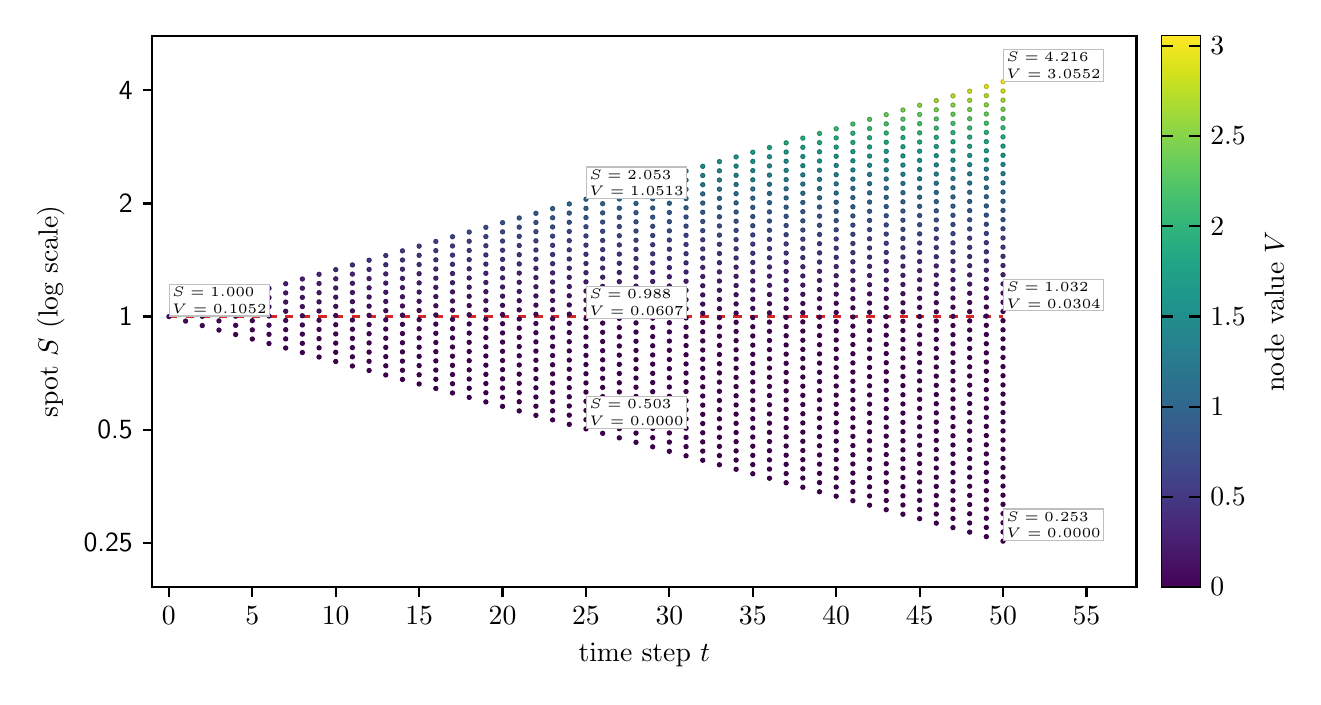
\begin{tikzpicture}
\begin{axis}[mpl, width=12.5cm, height=7cm, ymode=log, ytick={0.25,0.5,1,2,4}, yticklabels={0.25,0.5,1,2,4},
  xlabel={time step $t$}, ylabel={spot $S$ (log scale)}, xmin=-1, xmax=58, colormap/viridis, colorbar, set layers,
  colorbar style={ylabel={node value $V$}}, point meta min=0]
\addplot[scatter, only marks, mark=*, mark size=0.75pt, scatter src=explicit] table[x index=0, y index=1, meta index=2] {
0 1.00000 0.10520
1 0.97286 0.08721
1 1.02920 0.12318
2 0.94645 0.07123
2 1.00126 0.10319
2 1.05924 0.14317
3 0.92076 0.05723
3 0.97408 0.08523
3 1.03049 0.12115
3 1.09017 0.16518
4 0.89577 0.04516
4 0.94764 0.06930
4 1.00252 0.10116
4 1.06058 0.14115
4 1.12200 0.18922
5 0.87146 0.03493
5 0.92192 0.05538
5 0.97531 0.08322
5 1.03179 0.11910
5 1.09154 0.16320
5 1.15476 0.21523
6 0.84780 0.02644
6 0.89690 0.04343
6 0.94884 0.06734
6 1.00379 0.09909
6 1.06192 0.13911
6 1.12341 0.18730
6 1.18847 0.24317
7 0.82479 0.01953
7 0.87255 0.03334
7 0.92308 0.05351
7 0.97654 0.08117
7 1.03309 0.11701
7 1.09292 0.16120
7 1.15621 0.21339
7 1.22317 0.27296
8 0.80240 0.01405
8 0.84887 0.02501
8 0.89803 0.04167
8 0.95003 0.06535
8 1.00505 0.09699
8 1.06325 0.13704
8 1.12483 0.18536
8 1.18997 0.24143
8 1.25888 0.30448
9 0.78062 0.00982
9 0.82583 0.01829
9 0.87365 0.03174
9 0.92425 0.05161
9 0.97777 0.07909
9 1.03439 0.11490
9 1.09430 0.15917
9 1.15767 0.21155
9 1.22471 0.27131
9 1.29563 0.33766
10 0.75943 0.00664
10 0.80341 0.01300
10 0.84994 0.02358
10 0.89916 0.03989
10 0.95123 0.06332
10 1.00632 0.09486
10 1.06459 0.13494
10 1.12625 0.18341
10 1.19147 0.23968
10 1.26047 0.30294
10 1.33346 0.37237
11 0.73882 0.00433
11 0.78161 0.00895
11 0.82687 0.01704
11 0.87475 0.03011
11 0.92541 0.04967
11 0.97900 0.07697
11 1.03570 0.11275
11 1.09568 0.15713
11 1.15913 0.20969
11 1.22625 0.26967
11 1.29727 0.33620
11 1.37239 0.40855
12 0.71877 0.00272
12 0.76039 0.00595
12 0.80443 0.01195
12 0.85101 0.02214
12 0.90029 0.03809
12 0.95243 0.06126
12 1.00759 0.09268
12 1.06594 0.13281
12 1.12766 0.18145
12 1.19297 0.23794
12 1.26205 0.30140
12 1.33514 0.37100
12 1.41246 0.44609
13 0.69926 0.00163
13 0.73975 0.00380
13 0.78259 0.00810
13 0.82791 0.01580
13 0.87586 0.02847
13 0.92658 0.04771
13 0.98024 0.07481
13 1.03700 0.11056
13 1.09706 0.15506
13 1.16059 0.20783
13 1.22780 0.26804
13 1.29890 0.33477
13 1.37412 0.40724
13 1.45370 0.48495
14 0.68028 0.00093
14 0.71967 0.00233
14 0.76135 0.00528
14 0.80544 0.01091
14 0.85208 0.02069
14 0.90143 0.03626
14 0.95363 0.05915
14 1.00886 0.09047
14 1.06728 0.13065
14 1.12909 0.17947
14 1.19447 0.23620
14 1.26364 0.29989
14 1.33682 0.36965
14 1.41424 0.44483
14 1.49614 0.52507
15 0.66181 0.00050
15 0.70014 0.00136
15 0.74068 0.00330
15 0.78358 0.00726
15 0.82896 0.01456
15 0.87696 0.02682
15 0.92775 0.04570
15 0.98147 0.07260
15 1.03831 0.10833
15 1.09844 0.15297
15 1.16205 0.20597
15 1.22935 0.26643
15 1.30054 0.33335
15 1.37585 0.40594
15 1.45553 0.48371
15 1.53982 0.56644
16 0.64385 0.00025
16 0.68113 0.00075
16 0.72058 0.00197
16 0.76231 0.00464
16 0.80645 0.00989
16 0.85316 0.01923
16 0.90256 0.03440
16 0.95483 0.05700
16 1.01013 0.08820
16 1.06862 0.12845
16 1.13051 0.17748
16 1.19598 0.23446
16 1.26524 0.29839
16 1.33851 0.36831
16 1.41602 0.44358
16 1.49803 0.52384
16 1.58478 0.60904
17 0.62637 0.00012
17 0.66265 0.00039
17 0.70102 0.00111
17 0.74162 0.00282
17 0.78457 0.00645
17 0.83000 0.01332
17 0.87807 0.02514
17 0.92892 0.04366
17 0.98271 0.07035
17 1.03962 0.10606
17 1.09982 0.15085
17 1.16352 0.20411
17 1.23090 0.26482
17 1.30218 0.33195
17 1.37759 0.40467
17 1.45736 0.48248
17 1.54176 0.56520
17 1.63105 0.65287
18 0.60937 0.00005
18 0.64466 0.00019
18 0.68199 0.00059
18 0.72149 0.00163
18 0.76327 0.00402
18 0.80747 0.00888
18 0.85423 0.01777
18 0.90370 0.03251
18 0.95604 0.05481
18 1.01140 0.08589
18 1.06997 0.12623
18 1.13193 0.17548
18 1.19749 0.23274
18 1.26683 0.29691
18 1.34020 0.36700
18 1.41781 0.44234
18 1.49991 0.52262
18 1.58677 0.60778
18 1.67867 0.69796
19 0.59283 0.00002
19 0.62716 0.00008
19 0.66348 0.00029
19 0.70190 0.00089
19 0.74255 0.00238
19 0.78555 0.00566
19 0.83105 0.01210
19 0.87917 0.02345
19 0.93009 0.04157
19 0.98395 0.06804
19 1.04093 0.10374
19 1.10121 0.14871
19 1.16498 0.20224
19 1.23245 0.26323
19 1.30382 0.33058
19 1.37932 0.40342
19 1.45920 0.48127
19 1.54370 0.56397
19 1.63310 0.65159
19 1.72768 0.74433
20 0.57674 0.00001
20 0.61014 0.00003
20 0.64547 0.00013
20 0.68285 0.00045
20 0.72240 0.00132
20 0.76423 0.00343
20 0.80849 0.00789
20 0.85531 0.01631
20 0.90484 0.03059
20 0.95724 0.05256
20 1.01267 0.08353
20 1.07132 0.12396
20 1.13336 0.17346
20 1.19899 0.23102
20 1.26843 0.29545
20 1.34188 0.36571
20 1.41959 0.44113
20 1.50180 0.52141
20 1.58877 0.60654
20 1.68078 0.69665
20 1.77812 0.79201
21 0.56109 0.00000
21 0.59358 0.00001
21 0.62795 0.00005
21 0.66432 0.00021
21 0.70279 0.00069
21 0.74349 0.00196
21 0.78654 0.00490
21 0.83209 0.01088
21 0.88028 0.02173
21 0.93126 0.03944
21 0.98519 0.06567
21 1.04224 0.10138
21 1.10260 0.14654
21 1.16645 0.20038
21 1.23400 0.26167
21 1.30546 0.32923
21 1.38106 0.40218
21 1.46104 0.48007
21 1.54565 0.56275
21 1.63516 0.65032
21 1.72985 0.74299
21 1.83003 0.84103
22 0.54586 0.00000
22 0.57747 0.00000
22 0.61091 0.00002
22 0.64629 0.00009
22 0.68371 0.00033
22 0.72331 0.00105
22 0.76519 0.00287
22 0.80951 0.00692
22 0.85639 0.01484
22 0.90598 0.02863
22 0.95845 0.05025
22 1.01395 0.08110
22 1.07267 0.12165
22 1.13479 0.17143
22 1.20051 0.22932
22 1.27003 0.29401
22 1.34358 0.36444
22 1.42138 0.43993
22 1.50370 0.52021
22 1.59078 0.60529
22 1.68290 0.69535
22 1.78036 0.79063
22 1.88346 0.89143
23 0.53104 0.00000
23 0.56179 0.00000
23 0.59433 0.00001
23 0.62874 0.00003
23 0.66516 0.00014
23 0.70367 0.00052
23 0.74443 0.00158
23 0.78754 0.00417
23 0.83314 0.00967
23 0.88139 0.02000
23 0.93243 0.03726
23 0.98643 0.06324
23 1.04355 0.09895
23 1.10399 0.14435
23 1.16792 0.19852
23 1.23556 0.26012
23 1.30711 0.32790
23 1.38280 0.40097
23 1.46288 0.47888
23 1.54760 0.56154
23 1.63722 0.64905
23 1.73203 0.74164
23 1.83234 0.83961
23 1.93845 0.94325
24 0.51663 0.00000
24 0.54654 0.00000
24 0.57819 0.00000
24 0.61168 0.00001
24 0.64710 0.00006
24 0.68457 0.00023
24 0.72422 0.00080
24 0.76616 0.00235
24 0.81053 0.00598
24 0.85747 0.01337
24 0.90712 0.02664
24 0.95965 0.04788
24 1.01523 0.07861
24 1.07402 0.11930
24 1.13622 0.16940
24 1.20202 0.22764
24 1.27163 0.29261
24 1.34527 0.36320
24 1.42317 0.43875
24 1.50559 0.51902
24 1.59278 0.60405
24 1.68502 0.69404
24 1.78260 0.78925
24 1.88583 0.88997
24 1.99504 0.99652
25 0.50260 0.00000
25 0.53171 0.00000
25 0.56250 0.00000
25 0.59508 0.00000
25 0.62954 0.00002
25 0.66599 0.00009
25 0.70456 0.00037
25 0.74536 0.00123
25 0.78853 0.00347
25 0.83419 0.00849
25 0.88250 0.01825
25 0.93361 0.03502
25 0.98767 0.06074
25 1.04487 0.09647
25 1.10538 0.14213
25 1.16939 0.19667
25 1.23711 0.25861
25 1.30875 0.32661
25 1.38455 0.39979
25 1.46473 0.47771
25 1.54955 0.56033
25 1.63928 0.64778
25 1.73422 0.74030
25 1.83465 0.83819
25 1.94089 0.94175
25 2.05329 1.05130
26 0.48896 0.00000
26 0.51728 0.00000
26 0.54723 0.00000
26 0.57892 0.00000
26 0.61245 0.00001
26 0.64792 0.00003
26 0.68544 0.00015
26 0.72513 0.00059
26 0.76712 0.00187
26 0.81155 0.00507
26 0.85855 0.01190
26 0.90827 0.02460
26 0.96086 0.04544
26 1.01651 0.07604
26 1.07538 0.11691
26 1.13765 0.16736
26 1.20353 0.22597
26 1.27323 0.29124
26 1.34696 0.36199
26 1.42497 0.43759
26 1.50749 0.51784
26 1.59479 0.60282
26 1.68714 0.69274
26 1.78485 0.78787
26 1.88821 0.88851
26 1.99756 0.99498
26 2.11324 1.10762
27 0.47569 0.00000
27 0.50324 0.00000
27 0.53238 0.00000
27 0.56321 0.00000
27 0.59583 0.00000
27 0.63033 0.00001
27 0.66683 0.00006
27 0.70545 0.00025
27 0.74630 0.00092
27 0.78952 0.00282
27 0.83524 0.00732
27 0.88361 0.01648
27 0.93478 0.03272
27 0.98892 0.05815
27 1.04619 0.09393
27 1.10677 0.13989
27 1.17087 0.19483
27 1.23867 0.25712
27 1.31040 0.32535
27 1.38629 0.39862
27 1.46657 0.47655
27 1.55150 0.55912
27 1.64135 0.64651
27 1.73640 0.73897
27 1.83696 0.83678
27 1.94334 0.94025
27 2.05588 1.04971
27 2.17493 1.16552
28 0.46278 0.00000
28 0.48958 0.00000
28 0.51793 0.00000
28 0.54792 0.00000
28 0.57965 0.00000
28 0.61322 0.00000
28 0.64873 0.00002
28 0.68630 0.00009
28 0.72605 0.00041
28 0.76809 0.00144
28 0.81257 0.00420
28 0.85963 0.01044
28 0.90941 0.02253
28 0.96208 0.04292
28 1.01779 0.07339
28 1.07673 0.11446
28 1.13908 0.16531
28 1.20505 0.22434
28 1.27484 0.28990
28 1.34866 0.36080
28 1.42676 0.43644
28 1.50939 0.51666
28 1.59680 0.60159
28 1.68927 0.69144
28 1.78710 0.78649
28 1.89059 0.88706
28 2.00007 0.99344
28 2.11590 1.10599
28 2.23843 1.22505
29 0.45022 0.00000
29 0.47629 0.00000
29 0.50387 0.00000
29 0.53305 0.00000
29 0.56392 0.00000
29 0.59658 0.00000
29 0.63112 0.00000
29 0.66767 0.00003
29 0.70634 0.00016
29 0.74724 0.00066
29 0.79052 0.00222
29 0.83630 0.00619
29 0.88473 0.01470
29 0.93596 0.03035
29 0.99016 0.05548
29 1.04750 0.09131
29 1.10817 0.13762
29 1.17234 0.19301
29 1.24023 0.25568
29 1.31206 0.32413
29 1.38804 0.39748
29 1.46842 0.47540
29 1.55346 0.55793
29 1.64342 0.64525
29 1.73859 0.73763
29 1.83927 0.83536
29 1.94579 0.93875
29 2.05847 1.04813
29 2.17768 1.16384
29 2.30379 1.28626
30 0.43800 0.00000
30 0.46336 0.00000
30 0.49019 0.00000
30 0.51858 0.00000
30 0.54861 0.00000
30 0.58038 0.00000
30 0.61399 0.00000
30 0.64955 0.00001
30 0.68717 0.00005
30 0.72696 0.00027
30 0.76906 0.00106
30 0.81360 0.00338
30 0.86071 0.00899
30 0.91056 0.02040
30 0.96329 0.04030
30 1.01907 0.07065
30 1.07809 0.11197
30 1.14052 0.16327
30 1.20657 0.22274
30 1.27644 0.28861
30 1.35036 0.35965
30 1.42856 0.43531
30 1.51129 0.51549
30 1.59881 0.60036
30 1.69140 0.69014
30 1.78935 0.78512
30 1.89297 0.88560
30 2.00260 0.99190
30 2.11857 1.10436
30 2.24125 1.22333
30 2.37105 1.34919
31 0.42611 0.00000
31 0.45078 0.00000
31 0.47689 0.00000
31 0.50451 0.00000
31 0.53372 0.00000
31 0.56463 0.00000
31 0.59733 0.00000
31 0.63192 0.00000
31 0.66851 0.00001
31 0.70723 0.00009
31 0.74819 0.00044
31 0.79151 0.00167
31 0.83735 0.00509
31 0.88584 0.01290
31 0.93714 0.02791
31 0.99141 0.05269
31 1.04883 0.08861
31 1.10956 0.13532
31 1.17382 0.19121
31 1.24180 0.25428
31 1.31371 0.32294
31 1.38979 0.39636
31 1.47027 0.47426
31 1.55541 0.55673
31 1.64549 0.64398
31 1.74078 0.73629
31 1.84159 0.83395
31 1.94824 0.93726
31 2.06106 1.04655
31 2.18042 1.16217
31 2.30669 1.28449
31 2.44027 1.41389
32 0.41454 0.00000
32 0.43855 0.00000
32 0.46394 0.00000
32 0.49081 0.00000
32 0.51924 0.00000
32 0.54930 0.00000
32 0.58111 0.00000
32 0.61477 0.00000
32 0.65037 0.00000
32 0.68803 0.00002
32 0.72788 0.00016
32 0.77003 0.00073
32 0.81462 0.00261
32 0.86180 0.00756
32 0.91170 0.01823
32 0.96450 0.03759
32 1.02036 0.06780
32 1.07945 0.10941
32 1.14196 0.16123
32 1.20809 0.22119
32 1.27805 0.28736
32 1.35206 0.35852
32 1.43036 0.43419
32 1.51320 0.51433
32 1.60083 0.59913
32 1.69353 0.68884
32 1.79160 0.78375
32 1.89536 0.88415
32 2.00512 0.99036
32 2.12124 1.10273
32 2.24408 1.22161
32 2.37404 1.34737
32 2.51152 1.48041
33 0.40329 0.00000
33 0.42664 0.00000
33 0.45135 0.00000
33 0.47749 0.00000
33 0.50514 0.00000
33 0.53439 0.00000
33 0.56534 0.00000
33 0.59808 0.00000
33 0.63272 0.00000
33 0.66936 0.00000
33 0.70812 0.00004
33 0.74913 0.00027
33 0.79251 0.00119
33 0.83841 0.00404
33 0.88696 0.01109
33 0.93832 0.02538
33 0.99266 0.04979
33 1.05015 0.08582
33 1.11096 0.13301
33 1.17530 0.18945
33 1.24336 0.25293
33 1.31536 0.32179
33 1.39154 0.39525
33 1.47212 0.47312
33 1.55737 0.55553
33 1.64756 0.64272
33 1.74298 0.73496
33 1.84391 0.83253
33 1.95069 0.93576
33 2.06366 1.04497
33 2.18317 1.16050
33 2.30960 1.28272
33 2.44335 1.41202
33 2.58484 1.54880
34 0.39234 0.00000
34 0.41506 0.00000
34 0.43910 0.00000
34 0.46453 0.00000
34 0.49143 0.00000
34 0.51989 0.00000
34 0.55000 0.00000
34 0.58185 0.00000
34 0.61554 0.00000
34 0.65119 0.00000
34 0.68890 0.00001
34 0.72879 0.00008
34 0.77100 0.00046
34 0.81565 0.00191
34 0.86288 0.00616
34 0.91285 0.01601
34 0.96572 0.03475
34 1.02164 0.06483
34 1.08081 0.10680
34 1.14340 0.15921
34 1.20961 0.21970
34 1.27966 0.28616
34 1.35377 0.35743
34 1.43217 0.43308
34 1.51510 0.51317
34 1.60284 0.59790
34 1.69567 0.68754
34 1.79386 0.78237
34 1.89775 0.88270
34 2.00765 0.98883
34 2.12391 1.10111
34 2.24691 1.21989
34 2.37703 1.34555
34 2.51468 1.47848
34 2.66031 1.61912
35 0.38169 0.00000
35 0.40380 0.00000
35 0.42718 0.00000
35 0.45192 0.00000
35 0.47809 0.00000
35 0.50578 0.00000
35 0.53507 0.00000
35 0.56605 0.00000
35 0.59883 0.00000
35 0.63351 0.00000
35 0.67020 0.00000
35 0.70901 0.00002
35 0.75007 0.00014
35 0.79351 0.00078
35 0.83946 0.00305
35 0.88808 0.00927
35 0.93951 0.02275
35 0.99391 0.04674
35 1.05147 0.08292
35 1.11236 0.13068
35 1.17678 0.18775
35 1.24493 0.25164
35 1.31702 0.32069
35 1.39329 0.39417
35 1.47398 0.47199
35 1.55934 0.55434
35 1.64964 0.64146
35 1.74517 0.73362
35 1.84624 0.83112
35 1.95315 0.93427
35 2.06626 1.04339
35 2.18592 1.15883
35 2.31251 1.28095
35 2.44643 1.41015
35 2.58810 1.54682
35 2.73798 1.69142
36 0.37133 0.00000
36 0.39284 0.00000
36 0.41559 0.00000
36 0.43965 0.00000
36 0.46511 0.00000
36 0.49205 0.00000
36 0.52054 0.00000
36 0.55069 0.00000
36 0.58258 0.00000
36 0.61632 0.00000
36 0.65201 0.00000
36 0.68977 0.00000
36 0.72971 0.00003
36 0.77197 0.00025
36 0.81668 0.00130
36 0.86397 0.00481
36 0.91400 0.01374
36 0.96693 0.03177
36 1.02293 0.06172
36 1.08217 0.10413
36 1.14484 0.15723
36 1.21114 0.21827
36 1.28127 0.28502
36 1.35547 0.35635
36 1.43397 0.43198
36 1.51701 0.51201
36 1.60486 0.59668
36 1.69780 0.68624
36 1.79612 0.78100
36 1.90014 0.88124
36 2.01018 0.98729
36 2.12659 1.09948
36 2.24974 1.21817
36 2.38002 1.34373
36 2.51785 1.47656
36 2.66366 1.61709
36 2.81792 1.76575
37 0.36125 0.00000
37 0.38217 0.00000
37 0.40431 0.00000
37 0.42772 0.00000
37 0.45249 0.00000
37 0.47869 0.00000
37 0.50642 0.00000
37 0.53574 0.00000
37 0.56677 0.00000
37 0.59959 0.00000
37 0.63431 0.00000
37 0.67105 0.00000
37 0.70991 0.00000
37 0.75102 0.00006
37 0.79451 0.00045
37 0.84052 0.00215
37 0.88920 0.00747
37 0.94069 0.02001
37 0.99517 0.04352
37 1.05280 0.07991
37 1.11376 0.12835
37 1.17826 0.18611
37 1.24650 0.25042
37 1.31868 0.31961
37 1.39505 0.39309
37 1.47584 0.47087
37 1.56130 0.55315
37 1.65172 0.64020
37 1.74737 0.73229
37 1.84856 0.82971
37 1.95561 0.93278
37 2.06887 1.04181
37 2.18867 1.15716
37 2.31542 1.27918
37 2.44951 1.40828
37 2.59136 1.54485
37 2.74143 1.68932
37 2.90019 1.84217
38 0.35145 0.00000
38 0.37180 0.00000
38 0.39333 0.00000
38 0.41611 0.00000
38 0.44021 0.00000
38 0.46570 0.00000
38 0.49267 0.00000
38 0.52120 0.00000
38 0.55138 0.00000
38 0.58331 0.00000
38 0.61710 0.00000
38 0.65283 0.00000
38 0.69064 0.00000
38 0.73063 0.00001
38 0.77294 0.00011
38 0.81771 0.00078
38 0.86506 0.00352
38 0.91516 0.01141
38 0.96815 0.02861
38 1.02422 0.05843
38 1.08353 0.10140
38 1.14628 0.15530
38 1.21266 0.21692
38 1.28289 0.28393
38 1.35718 0.35530
38 1.43578 0.43088
38 1.51892 0.51085
38 1.60689 0.59545
38 1.69994 0.68495
38 1.79839 0.77963
38 1.90253 0.87979
38 2.01271 0.98576
38 2.12927 1.09786
38 2.25257 1.21645
38 2.38302 1.34191
38 2.52103 1.47464
38 2.66702 1.61505
38 2.82147 1.76360
38 2.98486 1.92074
39 0.34191 0.00000
39 0.36171 0.00000
39 0.38266 0.00000
39 0.40482 0.00000
39 0.42826 0.00000
39 0.45306 0.00000
39 0.47930 0.00000
39 0.50705 0.00000
39 0.53642 0.00000
39 0.56748 0.00000
39 0.60035 0.00000
39 0.63511 0.00000
39 0.67189 0.00000
39 0.71080 0.00000
39 0.75196 0.00001
39 0.79551 0.00021
39 0.84158 0.00136
39 0.89032 0.00568
39 0.94187 0.01714
39 0.99642 0.04009
39 1.05412 0.07677
39 1.11517 0.12603
39 1.17975 0.18456
39 1.24807 0.24928
39 1.32034 0.31857
39 1.39681 0.39202
39 1.47770 0.46974
39 1.56327 0.55196
39 1.65380 0.63894
39 1.74957 0.73096
39 1.85089 0.82830
39 1.95808 0.93129
39 2.07147 1.04023
39 2.19143 1.15549
39 2.31834 1.27742
39 2.45260 1.40641
39 2.59463 1.54287
39 2.74489 1.68723
39 2.90384 1.83996
39 3.07201 2.00153
40 0.33263 0.00000
40 0.35189 0.00000
40 0.37227 0.00000
40 0.39383 0.00000
40 0.41664 0.00000
40 0.44076 0.00000
40 0.46629 0.00000
40 0.49329 0.00000
40 0.52186 0.00000
40 0.55208 0.00000
40 0.58405 0.00000
40 0.61787 0.00000
40 0.65365 0.00000
40 0.69151 0.00000
40 0.73155 0.00000
40 0.77392 0.00003
40 0.81874 0.00038
40 0.86615 0.00233
40 0.91631 0.00904
40 0.96937 0.02525
40 1.02551 0.05493
40 1.08490 0.09862
40 1.14773 0.15345
40 1.21419 0.21568
40 1.28451 0.28289
40 1.35889 0.35426
40 1.43759 0.42979
40 1.52084 0.50969
40 1.60891 0.59423
40 1.70208 0.68365
40 1.80065 0.77826
40 1.90493 0.87834
40 2.01525 0.98423
40 2.13195 1.09624
40 2.25541 1.21474
40 2.38603 1.34010
40 2.52420 1.47272
40 2.67038 1.61302
40 2.82502 1.76145
40 2.98862 1.91847
40 3.16170 2.08458
41 0.32360 0.00000
41 0.34234 0.00000
41 0.36217 0.00000
41 0.38314 0.00000
41 0.40533 0.00000
41 0.42880 0.00000
41 0.45363 0.00000
41 0.47990 0.00000
41 0.50769 0.00000
41 0.53709 0.00000
41 0.56820 0.00000
41 0.60110 0.00000
41 0.63591 0.00000
41 0.67274 0.00000
41 0.71170 0.00000
41 0.75291 0.00000
41 0.79651 0.00006
41 0.84264 0.00070
41 0.89144 0.00396
41 0.94306 0.01411
41 0.99768 0.03638
41 1.05545 0.07347
41 1.11657 0.12376
41 1.18123 0.18314
41 1.24964 0.24822
41 1.32201 0.31756
41 1.39857 0.39096
41 1.47956 0.46862
41 1.56524 0.55077
41 1.65589 0.63768
41 1.75178 0.72963
41 1.85323 0.82689
41 1.96055 0.92980
41 2.07408 1.03866
41 2.19420 1.15382
41 2.32126 1.27565
41 2.45569 1.40454
41 2.59790 1.54090
41 2.74835 1.68515
41 2.90750 1.83775
41 3.07588 1.99919
41 3.25401 2.16998
42 0.31482 0.00000
42 0.33305 0.00000
42 0.35234 0.00000
42 0.37274 0.00000
42 0.39432 0.00000
42 0.41716 0.00000
42 0.44132 0.00000
42 0.46688 0.00000
42 0.49391 0.00000
42 0.52252 0.00000
42 0.55277 0.00000
42 0.58479 0.00000
42 0.61865 0.00000
42 0.65448 0.00000
42 0.69238 0.00000
42 0.73248 0.00000
42 0.77489 0.00000
42 0.81977 0.00012
42 0.86724 0.00129
42 0.91746 0.00662
42 0.97060 0.02161
42 1.02680 0.05115
42 1.08627 0.09579
42 1.14917 0.15173
42 1.21572 0.21454
42 1.28612 0.28189
42 1.36061 0.35323
42 1.43940 0.42870
42 1.52276 0.50854
42 1.61094 0.59300
42 1.70423 0.68236
42 1.80292 0.77689
42 1.90733 0.87690
42 2.01779 0.98269
42 2.13464 1.09462
42 2.25826 1.21302
42 2.38903 1.33828
42 2.52738 1.47080
42 2.67375 1.61099
42 2.82859 1.75930
42 2.99239 1.91620
42 3.16568 2.08218
42 3.34901 2.25778
43 0.30627 0.00000
43 0.32401 0.00000
43 0.34277 0.00000
43 0.36262 0.00000
43 0.38362 0.00000
43 0.40584 0.00000
43 0.42934 0.00000
43 0.45420 0.00000
43 0.48051 0.00000
43 0.50833 0.00000
43 0.53777 0.00000
43 0.56891 0.00000
43 0.60186 0.00000
43 0.63671 0.00000
43 0.67359 0.00000
43 0.71259 0.00000
43 0.75386 0.00000
43 0.79752 0.00000
43 0.84370 0.00024
43 0.89256 0.00234
43 0.94425 0.01090
43 0.99893 0.03231
43 1.05678 0.07000
43 1.11798 0.12159
43 1.18272 0.18187
43 1.25122 0.24722
43 1.32367 0.31655
43 1.40033 0.38990
43 1.48142 0.46749
43 1.56721 0.54958
43 1.65797 0.63642
43 1.75399 0.72830
43 1.85556 0.82549
43 1.96302 0.92831
43 2.07670 1.03708
43 2.19696 1.15215
43 2.32419 1.27389
43 2.45878 1.40268
43 2.60117 1.53892
43 2.75181 1.68306
43 2.91117 1.83554
43 3.07976 1.99685
43 3.25811 2.16751
43 3.44679 2.34805
44 0.29796 0.00000
44 0.31521 0.00000
44 0.33347 0.00000
44 0.35278 0.00000
44 0.37321 0.00000
44 0.39482 0.00000
44 0.41769 0.00000
44 0.44187 0.00000
44 0.46746 0.00000
44 0.49453 0.00000
44 0.52317 0.00000
44 0.55347 0.00000
44 0.58552 0.00000
44 0.61943 0.00000
44 0.65530 0.00000
44 0.69325 0.00000
44 0.73340 0.00000
44 0.77587 0.00000
44 0.82080 0.00000
44 0.86833 0.00047
44 0.91862 0.00421
44 0.97182 0.01759
44 1.02810 0.04702
44 1.08763 0.09297
44 1.15062 0.15020
44 1.21725 0.21353
44 1.28775 0.28091
44 1.36232 0.35219
44 1.44121 0.42761
44 1.52467 0.50738
44 1.61297 0.59178
44 1.70638 0.68107
44 1.80520 0.77552
44 1.90974 0.87545
44 2.02033 0.98116
44 2.13733 1.09300
44 2.26110 1.21131
44 2.39204 1.33647
44 2.53057 1.46888
44 2.67712 1.60896
44 2.83215 1.75715
44 2.99616 1.91393
44 3.16967 2.07978
44 3.35323 2.25524
44 3.54742 2.44085
45 0.28987 0.00000
45 0.30666 0.00000
45 0.32442 0.00000
45 0.34320 0.00000
45 0.36308 0.00000
45 0.38411 0.00000
45 0.40635 0.00000
45 0.42988 0.00000
45 0.45478 0.00000
45 0.48111 0.00000
45 0.50897 0.00000
45 0.53845 0.00000
45 0.56963 0.00000
45 0.60262 0.00000
45 0.63752 0.00000
45 0.67443 0.00000
45 0.71349 0.00000
45 0.75481 0.00000
45 0.79852 0.00000
45 0.84477 0.00000
45 0.89369 0.00095
45 0.94544 0.00747
45 1.00019 0.02772
45 1.05811 0.06633
45 1.11939 0.11962
45 1.18421 0.18079
45 1.25279 0.24627
45 1.32534 0.31555
45 1.40209 0.38884
45 1.48329 0.46637
45 1.56919 0.54840
45 1.66006 0.63517
45 1.75620 0.72697
45 1.85790 0.82408
45 1.96549 0.92682
45 2.07931 1.03551
45 2.19973 1.15049
45 2.32712 1.27213
45 2.46188 1.40082
45 2.60445 1.53695
45 2.75528 1.68097
45 2.91484 1.83334
45 3.08364 1.99452
45 3.26221 2.16504
45 3.45113 2.34543
45 3.65099 2.53627
46 0.28200 0.00000
46 0.29833 0.00000
46 0.31561 0.00000
46 0.33389 0.00000
46 0.35322 0.00000
46 0.37368 0.00000
46 0.39532 0.00000
46 0.41821 0.00000
46 0.44243 0.00000
46 0.46805 0.00000
46 0.49516 0.00000
46 0.52383 0.00000
46 0.55417 0.00000
46 0.58626 0.00000
46 0.62021 0.00000
46 0.65613 0.00000
46 0.69413 0.00000
46 0.73432 0.00000
46 0.77685 0.00000
46 0.82184 0.00000
46 0.86943 0.00000
46 0.91978 0.00190
46 0.97304 0.01305
46 1.02939 0.04239
46 1.08901 0.09026
46 1.15207 0.14897
46 1.21879 0.21261
46 1.28937 0.27994
46 1.36404 0.35116
46 1.44303 0.42651
46 1.52660 0.50623
46 1.61500 0.59056
46 1.70853 0.67978
46 1.80747 0.77416
46 1.91214 0.87400
46 2.02288 0.97963
46 2.14002 1.09138
46 2.26395 1.20960
46 2.39506 1.33466
46 2.53376 1.46697
46 2.68049 1.60694
46 2.83572 1.75501
46 2.99994 1.91166
46 3.17367 2.07738
46 3.35746 2.25270
46 3.55189 2.43817
46 3.75758 2.63438
47 0.27435 0.00000
47 0.29024 0.00000
47 0.30704 0.00000
47 0.32483 0.00000
47 0.34364 0.00000
47 0.36354 0.00000
47 0.38459 0.00000
47 0.40686 0.00000
47 0.43042 0.00000
47 0.45535 0.00000
47 0.48172 0.00000
47 0.50961 0.00000
47 0.53913 0.00000
47 0.57035 0.00000
47 0.60338 0.00000
47 0.63832 0.00000
47 0.67528 0.00000
47 0.71439 0.00000
47 0.75576 0.00000
47 0.79953 0.00000
47 0.84583 0.00000
47 0.89481 0.00000
47 0.94663 0.00380
47 1.00145 0.02229
47 1.05945 0.06249
47 1.12080 0.11804
47 1.18571 0.17989
47 1.25437 0.24533
47 1.32701 0.31455
47 1.40386 0.38778
47 1.48516 0.46525
47 1.57117 0.54721
47 1.66215 0.63391
47 1.75841 0.72564
47 1.86024 0.82268
47 1.96797 0.92533
47 2.08194 1.03394
47 2.20250 1.14883
47 2.33005 1.27037
47 2.46499 1.39895
47 2.60773 1.53498
47 2.75875 1.67889
47 2.91851 1.83113
47 3.08752 1.99219
47 3.26632 2.16257
47 3.45548 2.34282
47 3.65559 2.53351
47 3.86729 2.73525
48 0.26690 0.00000
48 0.28236 0.00000
48 0.29871 0.00000
48 0.31601 0.00000
48 0.33431 0.00000
48 0.35367 0.00000
48 0.37415 0.00000
48 0.39582 0.00000
48 0.41874 0.00000
48 0.44299 0.00000
48 0.46864 0.00000
48 0.49578 0.00000
48 0.52449 0.00000
48 0.55487 0.00000
48 0.58700 0.00000
48 0.62099 0.00000
48 0.65696 0.00000
48 0.69500 0.00000
48 0.73525 0.00000
48 0.77783 0.00000
48 0.82287 0.00000
48 0.87052 0.00000
48 0.92094 0.00000
48 0.97427 0.00760
48 1.03069 0.03699
48 1.09038 0.08799
48 1.15352 0.14810
48 1.22032 0.21169
48 1.29099 0.27896
48 1.36576 0.35013
48 1.44485 0.42542
48 1.52852 0.50508
48 1.61704 0.58934
48 1.71068 0.67849
48 1.80975 0.77279
48 1.91455 0.87256
48 2.02543 0.97811
48 2.14272 1.08976
48 2.26681 1.20789
48 2.39808 1.33285
48 2.53695 1.46505
48 2.68387 1.60491
48 2.83929 1.75287
48 3.00372 1.90939
48 3.17767 2.07498
48 3.36169 2.25016
48 3.55637 2.43549
48 3.76232 2.63154
48 3.98020 2.83895
49 0.25966 0.00000
49 0.27469 0.00000
49 0.29060 0.00000
49 0.30743 0.00000
49 0.32523 0.00000
49 0.34407 0.00000
49 0.36399 0.00000
49 0.38507 0.00000
49 0.40737 0.00000
49 0.43097 0.00000
49 0.45592 0.00000
49 0.48233 0.00000
49 0.51026 0.00000
49 0.53981 0.00000
49 0.57107 0.00000
49 0.60414 0.00000
49 0.63912 0.00000
49 0.67614 0.00000
49 0.71529 0.00000
49 0.75671 0.00000
49 0.80054 0.00000
49 0.84690 0.00000
49 0.89594 0.00000
49 0.94782 0.00000
49 1.00271 0.01519
49 1.06078 0.05878
49 1.12221 0.11720
49 1.18720 0.17900
49 1.25595 0.24438
49 1.32869 0.31355
49 1.40563 0.38672
49 1.48703 0.46413
49 1.57315 0.54602
49 1.66425 0.63266
49 1.76063 0.72431
49 1.86259 0.82127
49 1.97045 0.92385
49 2.08456 1.03236
49 2.20528 1.14716
49 2.33299 1.26861
49 2.46809 1.39709
49 2.61102 1.53302
49 2.76223 1.67681
49 2.92219 1.82893
49 3.09142 1.98986
49 3.27044 2.16011
49 3.45983 2.34022
49 3.66020 2.53076
49 3.87216 2.73233
49 4.09640 2.94557
50 0.25261 0.00000
50 0.26724 0.00000
50 0.28271 0.00000
50 0.29909 0.00000
50 0.31641 0.00000
50 0.33473 0.00000
50 0.35411 0.00000
50 0.37462 0.00000
50 0.39632 0.00000
50 0.41927 0.00000
50 0.44355 0.00000
50 0.46923 0.00000
50 0.49641 0.00000
50 0.52515 0.00000
50 0.55557 0.00000
50 0.58774 0.00000
50 0.62178 0.00000
50 0.65778 0.00000
50 0.69588 0.00000
50 0.73618 0.00000
50 0.77881 0.00000
50 0.82391 0.00000
50 0.87162 0.00000
50 0.92210 0.00000
50 0.97550 0.00000
50 1.03199 0.03039
50 1.09175 0.08716
50 1.15498 0.14723
50 1.22186 0.21077
50 1.29262 0.27799
50 1.36748 0.34910
50 1.44667 0.42434
50 1.53045 0.50392
50 1.61908 0.58812
50 1.71284 0.67720
50 1.81203 0.77143
50 1.91697 0.87112
50 2.02798 0.97658
50 2.14542 1.08815
50 2.26966 1.20618
50 2.40110 1.33105
50 2.54015 1.46314
50 2.68725 1.60289
50 2.84287 1.75073
50 3.00750 1.90713
50 3.18167 2.07259
50 3.36592 2.24763
50 3.56085 2.43280
50 3.76706 2.62871
50 3.98521 2.83595
50 4.21600 3.05520
};
\addplot[tabred, dashed, line width=0.8pt] coordinates {(0,1) (50,1)};
\begin{pgfonlayer}{axis foreground}
\node[font=\tiny, align=left, fill=white, draw=black!25, inner sep=1pt, anchor=south west] at (axis cs:0,1.00000) {$S=1.000$\\ $V=0.1052$};
\node[font=\tiny, align=left, fill=white, draw=black!25, inner sep=1pt, anchor=south west] at (axis cs:25,0.50260) {$S=0.503$\\ $V=0.0000$};
\node[font=\tiny, align=left, fill=white, draw=black!25, inner sep=1pt, anchor=south west] at (axis cs:25,0.98767) {$S=0.988$\\ $V=0.0607$};
\node[font=\tiny, align=left, fill=white, draw=black!25, inner sep=1pt, anchor=south west] at (axis cs:25,2.05329) {$S=2.053$\\ $V=1.0513$};
\node[font=\tiny, align=left, fill=white, draw=black!25, inner sep=1pt, anchor=south west] at (axis cs:50,0.25261) {$S=0.253$\\ $V=0.0000$};
\node[font=\tiny, align=left, fill=white, draw=black!25, inner sep=1pt, anchor=south west] at (axis cs:50,1.03199) {$S=1.032$\\ $V=0.0304$};
\node[font=\tiny, align=left, fill=white, draw=black!25, inner sep=1pt, anchor=south west] at (axis cs:50,4.21600) {$S=4.216$\\ $V=3.0552$};
\end{pgfonlayer}
\end{axis}
\end{tikzpicture}
\captionof{figure}{Calibrated tree, $N=50$ ($u=1.029196$): all nodes, colour $=V$; red dashed line: strike $K=1$.}\label{fig:T50}
\end{center}

\par\medskip\noindent\textbf{Reading.}
\begin{itemize}
\item \emph{Root.} For $N=2,5,50$ the root value is $0.105195=V^*$: the calibration of Q1 at work.
\item \emph{Backward step.} Each node is the average of its two children ($\tilde p=\tilde q=\frac12$, Definition~2; the price tree is discounted to $t=0$, so no factor is applied inside the tree). $N=2$, root:
\begin{align*}
\tfrac12\,(0.014334+0.196057) &= 0.105195 . && \checkmark
\end{align*}
\item \emph{Leaves.} A leaf is the payoff times $DF^N=DF_1^{\,T}=0.95$ (cell 8; Definition~3): $N=5$, $S=1.126288$:
\begin{align*}
0.95\,(1.126288-1) &= 0.119973 . && \checkmark
\end{align*}
Leaves below $K$ are worth $0$; only the orange leaves (Figures~\ref{fig:T2}, \ref{fig:T5}) feed the price.
\item \emph{Shape.} With more steps the up step shrinks ($1.1758$, $1.0972$, $1.0292$), but the leaves spread more ($0.253$ to $4.216$ for $N=50$); in log scale the tree is a symmetric fan around the growth of the money market (Lemma~2).
\end{itemize}

\ansbox{\textbf{Q4 (trees).} The pictures show the calibrated model at work: the leaves carry the discounted payoff, each node is the average of its two children, and the root is the given price $0.105195$ for every $N$.}

% ============================================================================ conclusions
\subhead{Conclusions.}
\ansbox{\begin{itemize}
\item \texttt{calibrate} (Q1) returns the up step of the balanced tree with the given call price: Steps 1--5 of Figure~\ref{fig:cal}, error at most $10^{-10}$ (in Demo A at most $7.1\cdot10^{-16}$).
\item Only prices between the tree prices at the two ends of the interval of $u$ can be calibrated (Step 2); other prices raise \texttt{ValueError}.
\item Every calibrated $u$ agrees with a second root solver (\texttt{brentq}) to $10^{-9}$ (Q1, Q3).
\item Demo A: with more steps the calibrated tree volatility tends to $\sigma=0.2$ of the market price (Q2).
\item Demo B: a one-step tree needs a different step for each strike and expiry (Q3).
\item Trees (Q4): in every calibrated tree the root is the given price, built backward from the discounted payoffs at the leaves.
\end{itemize}}

% ============================================================================ comment
\subhead{Comment (to keep in mind).}
\begin{itemize}
\item \emph{Why the bracket of Step 3.} The first tries applied \texttt{minimize} (L-BFGS-B, Nelder--Mead) on all of $(1/DF,2/DF)$: they can stop in the flat part, where the error is constant and the gradient is zero, and L-BFGS-B (finite-difference gradient) also stopped at errors of order $10^{-9}$. Inside the bracket this cannot happen. A root solver on $V(u)-V^*$ in the bracket (e.g.\ \texttt{scipy.optimize.brentq}) is an alternative.
\item \emph{Lecture code.} \texttt{create\_discounted\_price\_tree} reads the up step as \texttt{spot\_tree[1][-1]}$\,=uS_0$, which is $u$ only for $S_0=1$ (all runs here use $S_0=1$); and it multiplies $\tilde p$ with the down child (index $i$ counts up moves), which does not matter here because the tree is balanced, $\tilde p=\tilde q=\frac12$.
\end{itemize}

\subhead{References.}
\begin{enumerate}[label={[\arabic*]}]
\item Lecture~4 of this course: \texttt{Tree.ipynb} and \texttt{Binomial\_tree\_coding.ipynb}, repository QuantCourseBP, folder \texttt{Lectures/2026\_fall\_BME/04\_Tree}.
\item Earlier edition of the same tree lecture: \texttt{Tree.ipynb}, repository QuantCourseBP, folder \texttt{Lectures/2023\_fall\_ELTE/07\_Tree} (section ``Basic concept of binomial tree model (cont.)'').
\item S.~E.~Shreve, \emph{Stochastic Calculus for Finance I: The Binomial Asset Pricing Model}, Springer, 2004 (the literature of the lecture, \texttt{Tree.ipynb} cell 58), Chapter~1.
\item Homework~1 (Lesson~3) and Homework~2, Part~1 (Background) of this course.
\end{enumerate}

\end{document}
